\chapter[Introduction]{Introduction}
\chaptermark{Introduction}
\label{chap:introduction}
% TODO: remove
%And Schmidhuber said, Let there be backpropagation, and there was backpropagation.
\minitoc

\paragraph{Disclaimer} While vast parts in this \chapref{chap:introduction} are novel, and references were added otherwise, some parts were re-utilized from~\cite{huber2021homographybased, huber2022deep, huber2023deep} to remove redundancy from the introduction and methods sections of the chapters largely based on these publications.

\section{Foreword}
\label{in:sec:foreword}
This thesis investigates data driven endoscopic camera motion automation by means of a robot and therefore falls into the realm of \gls{ras}. Through research on robotics and computer vision, the research aims to find novel ways to support clinical staff in their surgical work by alleviating the burden of unfulfilling and repeatable tasks.

In \gls{ras}, it is commonly acknowledged that automation will proceed stepwise. From no autonomy to full automation, these steps are often categorized into six stages~\cite{zhang2017automation, fosch2021human}:
\begin{enumerate}
    \item No autonomy: Surgeon is in full charge of the robot
    \item Robot assistance: Robot constrains motion and corrects surgeon  
    \item Task autonomy: Robot executes specific tasks autonomously under human supervision
    \item Conditional autonomy: Robot plans and executes tasks under human approval
    \item High autonomy: Conditional autonomy without approval but with human intervention
    \item Full automation: Robot performs an entire surgery autonomously
\end{enumerate}
This thesis explores level five, high autonomy, which would require approval-free endoscopic camera motion execution with the possibility of human intervention. Although some works~\cite{battaglia2021rethinking} argue that the focus should not lie on automation, but enhancement, we adopt a futuristic sentiment and are in alignment with~\cite{kitaguchi2022artificial}, where the authors explain why camera motion automation will likely be achieved first. This futuristic notion follows previous surgical revolutions, from the advancement of open surgery to \gls{mis}, and the success of the da Vinci\textsuperscript{\textregistered} surgical robot in \gls{rmis}, see also \figref{in:fig:camera_motion_automation} and \figref{in:fig:robotic_vs_laparoscopic_vs_open}.
\begin{figure}[htb]
    \centering
    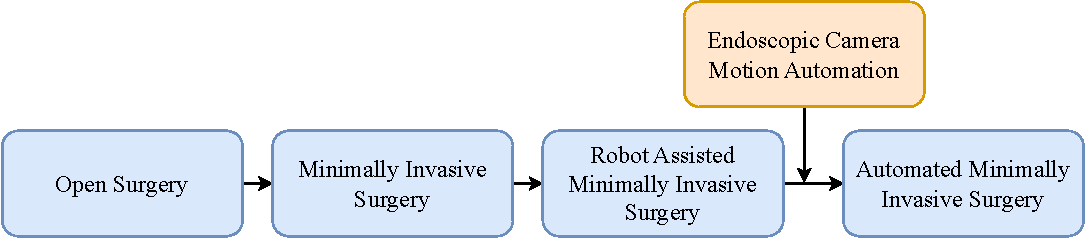
\includegraphics[width=0.9\textwidth]{introduction/fig/24_02_13_surgical_revolution.pdf}
    \caption{The gradual introduction of novel technology into the surgical field, one enabling the next. Endoscopic camera motion automation is likely to appear first towards full automation. Refers to \secref{in:sec:foreword}.}
    \label{in:fig:camera_motion_automation}
\end{figure}

The ever evolving field of surgery has repeatedly demonstrated acceptance of new technology~\cite{attanasio2021autonomoy}, and we argue that automation is no exception. The growth of \gls{rmis} can clearly be considered an enabling factor for full automation, see also \figref{in:fig:camera_motion_automation}.

When compared to other domains, such as autonomous driving, service and household robots, where robots already exert a significant amount autonomy that far exceeds \gls{rmis}, it becomes evident that advances in autonomy will ultimately make their way into the operating theater as well. Regulatory and economic hurdles cause delays in the adoption of novel technology by healthcare systems and hospital units. However, there might even be a future where \gls{rmis} will not only adopt full automation from other domains but make significant contributions to general machine intelligence. 

%Others~\cite{lecun2022path} have
\citet{lecun2022path}
argued that machines will need to interact with the real world in order to become truly intelligent and, arguably, \gls{rmis} has grown to be the most advanced \gls{phri} domain with thousands of deployed robots.
\begin{figure}[tbh]
    \centering
    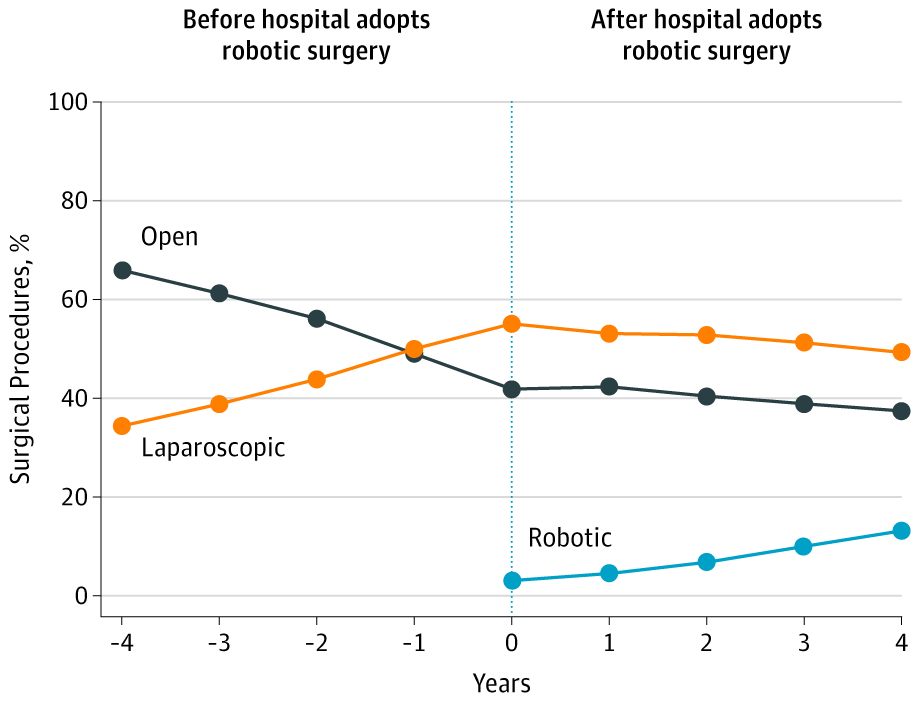
\includegraphics[width=0.6\textwidth]{introduction/img/robotic_since_introduction.png}
    \caption{Increase of laparoscopy over open approaches and robotic laparoscopy versus other methods, respectively. Data normalized to year zero, the introduction of robotic laparoscopy. The use of robotic laparoscopy increased from $1.8\%$ to $15.1\%$. For inguinal hernia repair, an increase in robotic surgery from $0.7\%$ to $28.8\%$ was found. A total of $169.404$ cases over 73 hospitals in Michigan, United States, were investigated. Figure and data provided with courtesy of~\cite{sheetz2020trends}. Refers to \secref{in:sec:foreword}.}
    \label{in:fig:robotic_vs_laparoscopic_vs_open}
\end{figure}

As we dive deeper into level five autonomy endoscopic camera motion automation, this introductory chapter will provide a necessary clinical background for laparoscopy in \secref{in:sec:laparoscopy}, a sub-domain of endoscopy, including an in-depth explanation of laparoscopic cholecystectomy (minimally invasive gallbladder removal). Laparoscopic cholecystectomy is the most commonly performed laparoscopic procedure~\cite{sheetz2020trends}, and can be considered relatively simple. Therefore, due to vast amounts of readily available data, it serves as the perfect test-bed for the methods that are derived as part of this thesis. 

Next, we explain the rise of robot assisted laparoscopy in \secref{in:sec:robot_assisted_laparoscopy} and the potentials of automation that evolve with it. We highlight different commercial systems, their limitations, and propose innovative solutions. Identified limitations will include spatial awareness, refer \secref{in:sec:spatial_awareness}, as most \gls{rmis} systems lack a world model, and, crucially, camera motion automation, for which a thorough review of related methods is provided in \secref{in:sec:camera_motion_automation}. Following the camera motion automation literature review, we will hypothesize an approach to near-term full automation. The proposed approach will revolve around a mixture of imitation learning an classical control. It is grounded in successful automation in related domains and will be discussed in \secref{in:sec:imitation_learning_for_camera_motion_automation}.

\section{Laparoscopy}
\label{in:sec:laparoscopy}
Endoscopy refers to the observation of internal parts by means of an endoscope~\cite{oedendoscopy}. The word endoscopy derives from the Greek by combining the prefix "endo" meaning "within" and the verb "skopein", "to view or observe"~\cite{majumdar1993short}. In the surgical context, endoscopy refers to a \gls{mis} procedure with the goal to observe within the body using a rigid endoscope. Surgical endoscopy inside the abdominal (belly) or pelvic (hip) cavity is called laparoscopy. During laparoscopy, an rigid endoscope, called laparoscope in this clinical context, is inserted through small incisions for diagnostic or interventional purposes, see \figref{in:fig:laparoscopy}.
\begin{figure}[tb]
    \centering
    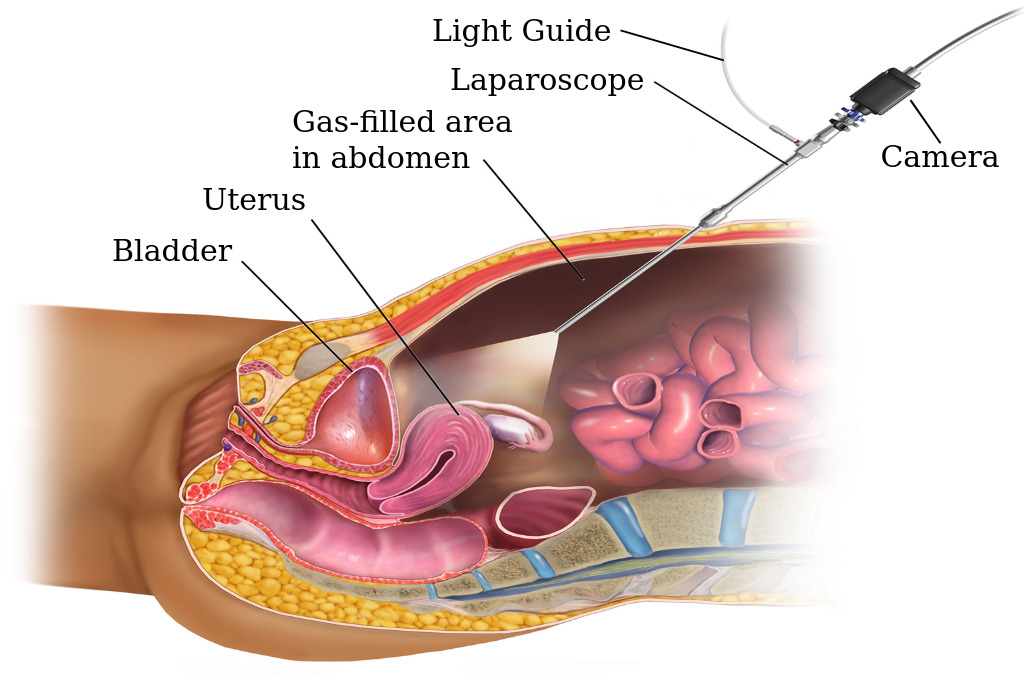
\includegraphics[width=0.7\textwidth]{introduction/img/laparoscopy.jpg}
    \caption{Illustration of a laparoscopic procedure. The laparoscope is inserted through a small incision in the patient's abdominal wall and provides a view of the surgical scene. To provide space, carbon dioxide ($\text{CO}_2$) is injected through a needle into the abdomen. Image provided with courtesy of~\cite{blausen2014laparoscopy}. Refers to \secref{in:sec:laparoscopy}.}
    \label{in:fig:laparoscopy}.
\end{figure}

Compared to open surgery, laparoscopy leads to significantly faster interventions ($57.19\pm10.13\,\text{min}$ vs. $85.10\pm15.18\,\text{min}$), less bleeding complications ($2\%$ vs $7\%$ of interventions), shorter hospital stays ($2.1\pm1.1\,\text{days}$ vs $4.4\pm2.1\,\text{days}$), less infections, and less post-operative pain~\cite{shi2023laparoscopic}. These eminent advantages of laparoscopic over open techniques have led to their adoption since their introduction in the early 1980s, see \figref{in:fig:robotic_vs_laparoscopic_vs_open}. This trend is foreseen to continue and even increase as the majority of surgical residents is nowadays trained on the minimally invasive procedure variants~\cite{john2020rise}.

Some types of laparoscopic procedures are cholecystectomy (gallbladder removal), appendectomy (appendix removal), inguinal hernia repair (i.e. leaking of intestines through the abdominal wall), colectomy (partial colon removal), nephrectomy (partial or complete kidney removal), prostatectomy (partial or complete prostate removal), adrenalectomy (removal of the adrenal gland), and gastrectomy (partial or full stomach removal) among others. Since laparoscopic cholecystectomy is carried out in high volumes and is additionally a relatively simple procedure, it is of special relevance to this work. It will thus be considered an example for explaining a laparoscopic surgery setup and procedure.

Cholecystectomy is the surgical removal of the gallbladder. The gallbladder serves as a reservoir for the liver-produced bile, a fat digesting fluid. Bile may harden and form gallstones, which can lead to inflammation and severe pain. Since the liver also releases bile directly into the digestive tract, shown in \figref{in:fig:cholecystectomy_incisions}, the gallbladder may be removed when necessary. A cholecystectomy setup is depicted in \figref{in:fig:room_setup}.
\begin{figure}[tb]
    \centering
    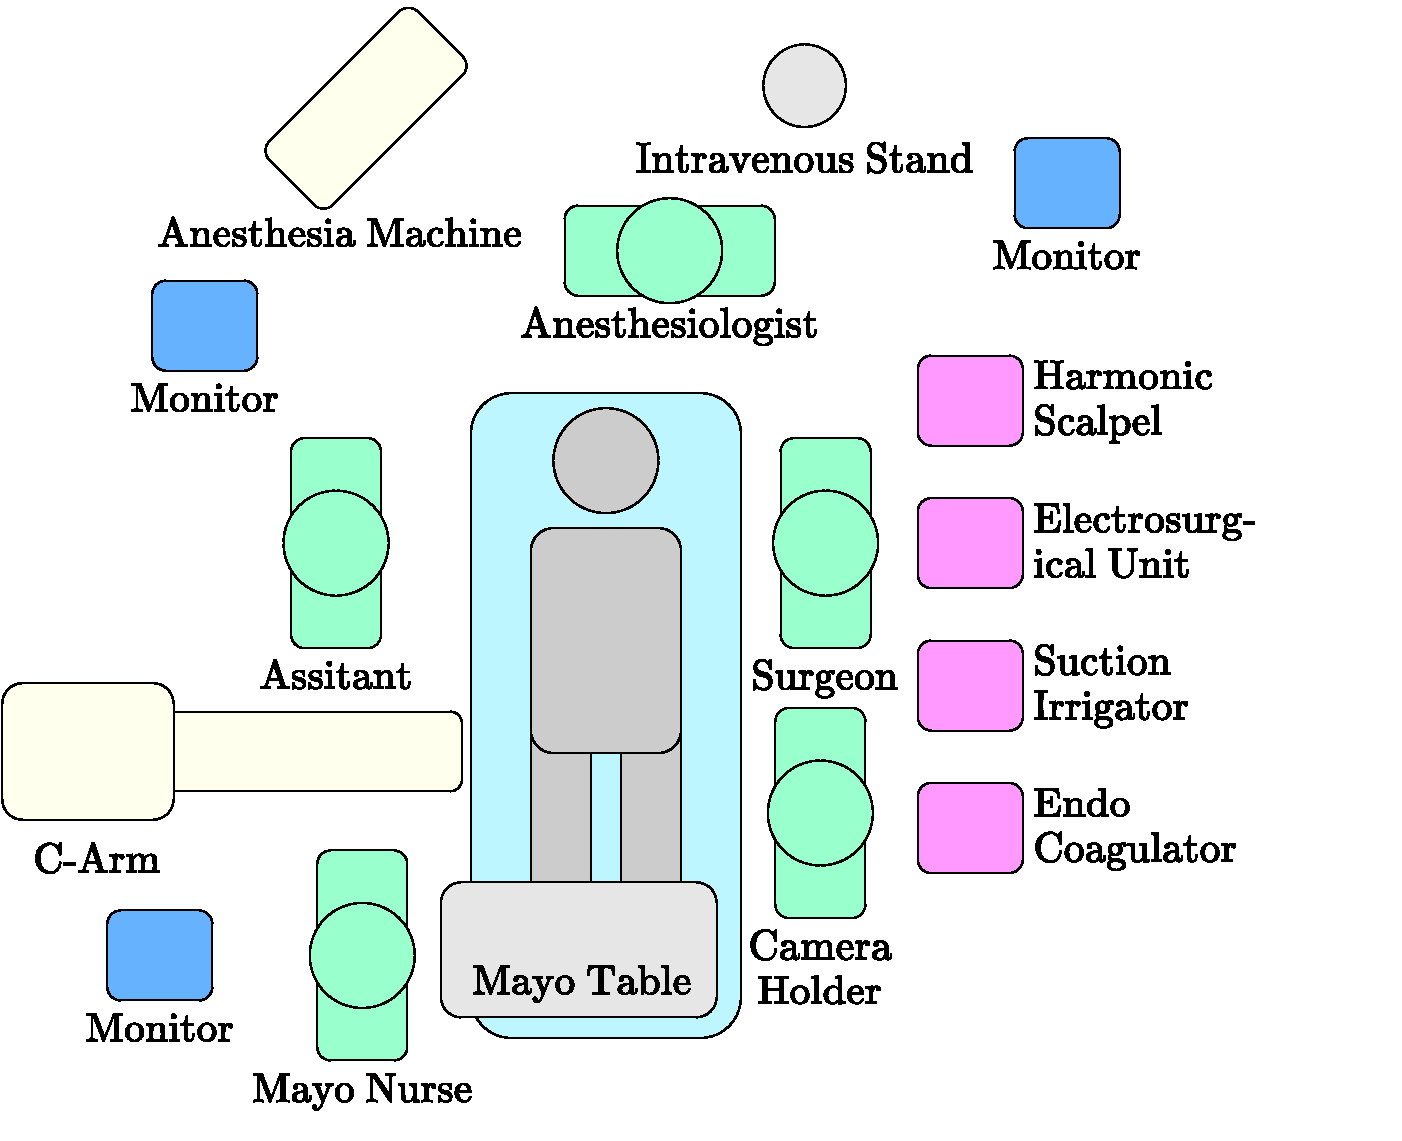
\includegraphics[width=0.7\textwidth]{introduction/fig/24_01_26_room_setup.pdf}
    \caption{Typical setup for a cholecystectomy. Image adapted from~\cite{sages2010room}. Refers to \secref{in:sec:cholecystectomy_setup}.}
    \label{in:fig:room_setup}
\end{figure}
\subsection{Laparoscopic Cholecystectomy Setup}
\label{in:sec:cholecystectomy_setup}

Even this relatively simple procedure requires multiple skilled practitioners. The surgeon is supported by an endoscope holder, a second assistant, an anesthesiologist, and a mayo nurse (for providing tools). The procedure commonly requires a harmonic scalpel, which cauterizes tissue and coagulates blood (i.e. causes blood clothing) through ultra-sonic waves. Due to lower cost for cauterization and coagulation, it may be preferable to use an electrosurgical unit (ESU), which generates different electrical waveforms and can be connected to most laparoscopic tools~\cite{archana2018comparing}. Further devices include a suction-irrigator for removing body fluids from the surgical scene, as well as an endoscopic camera system, a light source, and multiple monitors. A laparoflator is used to insulflate the abdomen with $\text{CO}_2$ and to maintain a fixed pressure. An anesthesia machine and an intravenous stand are utilized to regulate the patient's conditions. Finally, a C-arm may visualise the bile duct to probe for possible injuries and leakage caused by the intervention~\cite{cuschieri1994intraoperative}. The procedure is then referred to as cholangiography (x-ray visualization of the bile duct with contrast agent).

\subsection{Laparoscopic Cholecystectomy Procedure}
\label{in:sec:cholecystectomy_procedure}
\begin{figure}[tb]
    \centering
    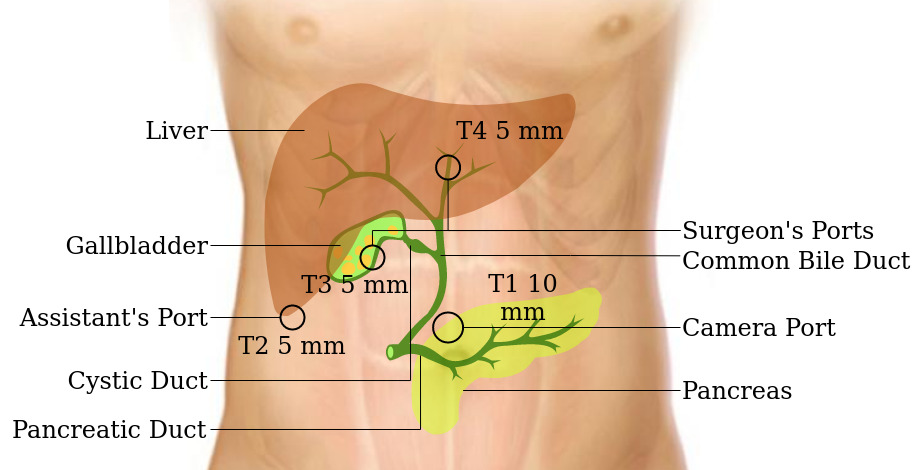
\includegraphics[width=0.9\textwidth]{introduction/fig/24_01_26_cholecystectomy_incisions.jpg}
    \caption{Common cholecystectomy incisions. Several incisions are made for the trocars T1-T4. Image with courtesy of~\cite{ALES5766} and modified to include port descriptions and organs. Refers to \secref{in:sec:cholecystectomy_procedure}}
    \label{in:fig:cholecystectomy_incisions}
\end{figure}

This paragraph explains laparoscopic cholecystectomy in simplified terms and vastly refers to~\cite{ALES5766}. To begin with, $\text{CO}_2$ is injected into the abdomen via a needle. The pressure is controlled through the laparoflator, see \figref{in:fig:room_setup}. Next, four small incisions are made for trocars T1-T4, which serve as entry point through the abdominal wall, shown in \figref{in:fig:cholecystectomy_incisions}. A laparoscope is inserted through T1 to grant an adequate view of the surgical scene. A grasper is inserted through T2 and used by the assistant to elevate the gallbladder. Trocars T3 and T4 are used by the surgeon to perform the cholecystectomy. It is important to identify anatomical landmarks before other steps are attempted. A good exposure of the surgical area is achieved through adequate patient and port positioning~\cite{gupta2023achieve}. Following the preparatory steps, the surgery can broadly be partitioned into six steps. These steps will be explained in the following.

\subsubsection{Step 1: Dissection of the Hepatocystic Triangle}
The goal is to expose the hepatocystic triangle~\cite{mischinger2020critical}, see \figref{in:fig:hepatocystic_triangle}. The gallbladder is gently pulled upward over the liver and its neck is pulled downward to expose its different parts, as can be seen in \figref{in:fig:cholecystectomy_incisions}. Swollen gallbladders are precautiously decompressed with a needle to prevent perforation with leakage of bile and gallstones. Potential adhesions (scarred connections to other organs) are carefully separated using cautery and regular tools, avoiding the area near the duodenum (beginning of the small intestine). Next, the hepatocystic triangle is dissected by carefully removing fibrous and fatty tissue. It is of utmost importance that no tubular structure may be damaged until cystic duct and cystic artery are identified~\cite{mischinger2020critical}.
\begin{figure}[tb]
    \centering
    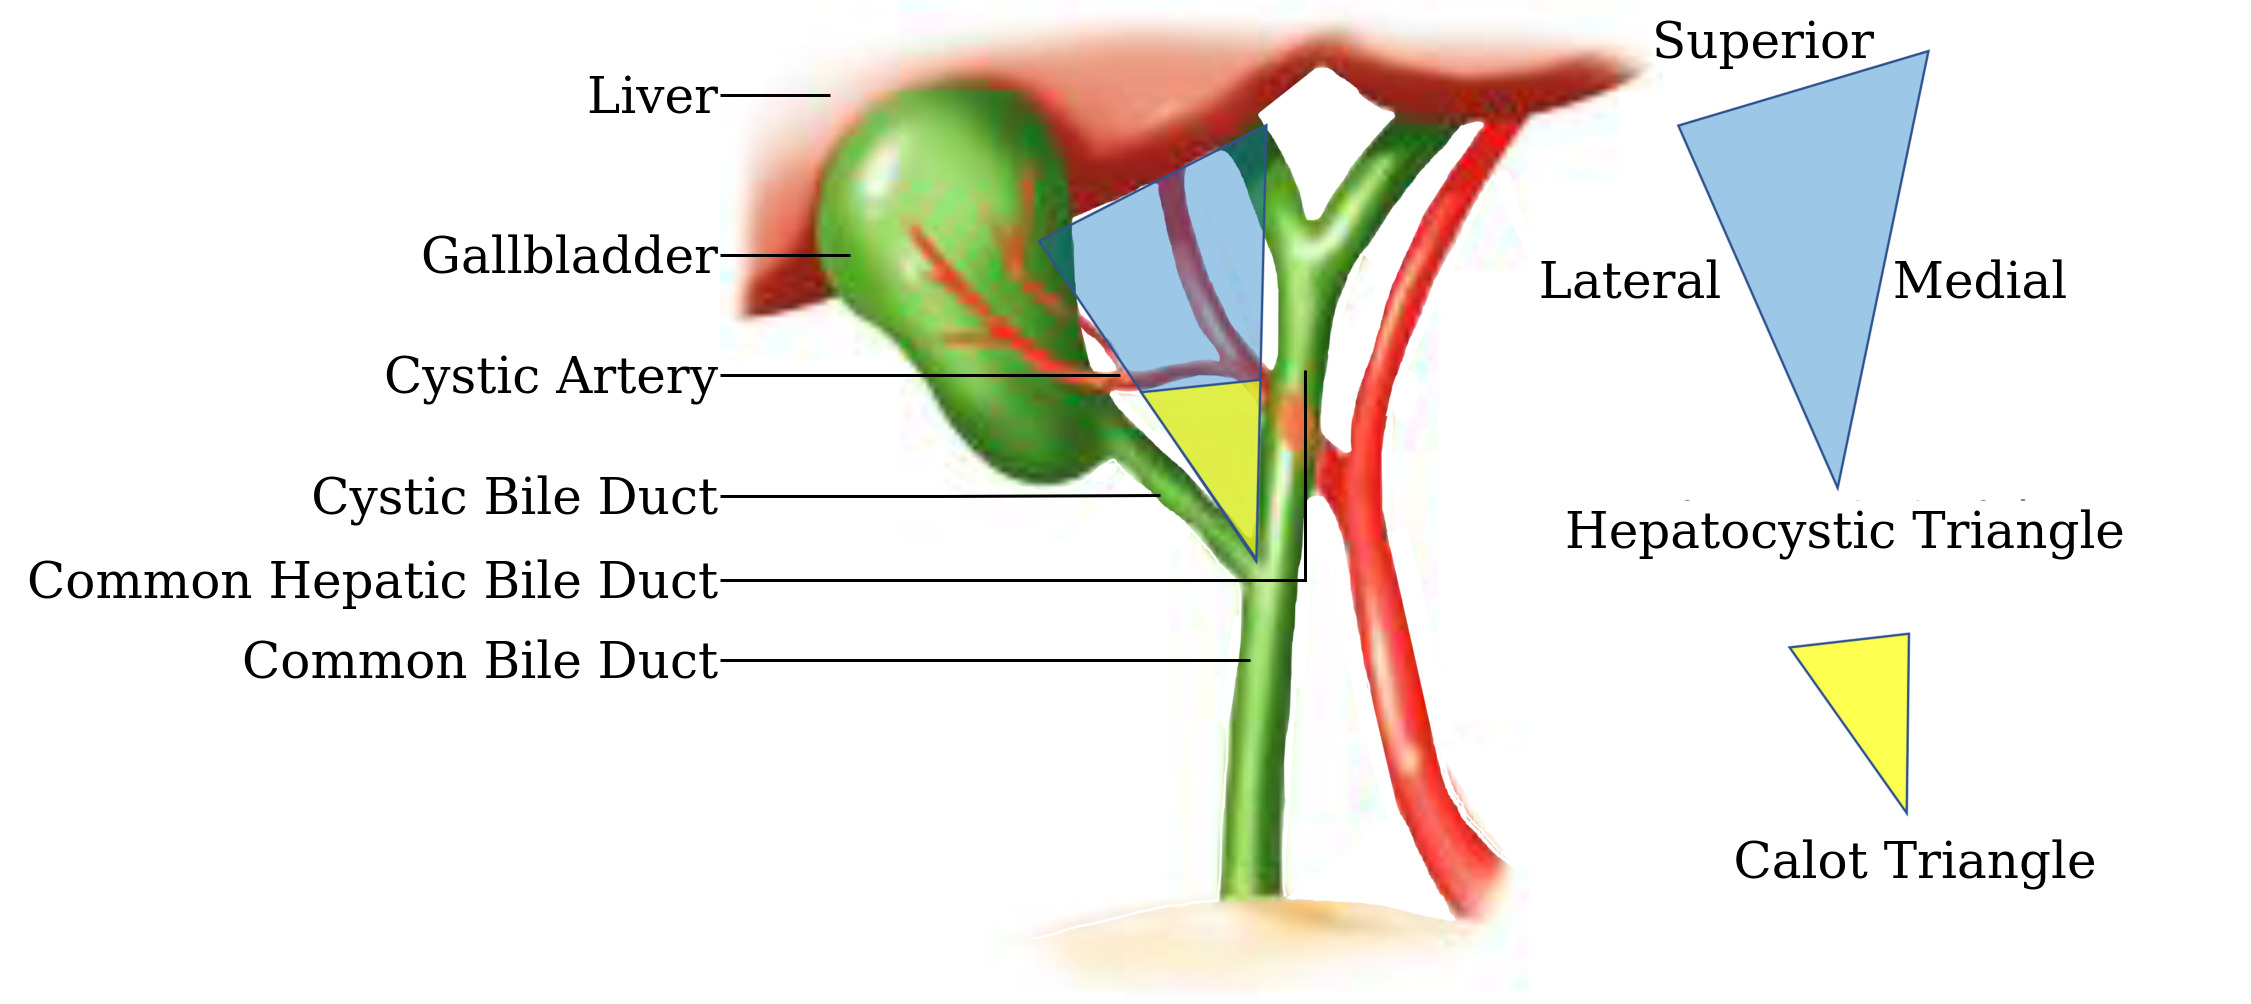
\includegraphics[width=0.8\textwidth]{introduction/fig/24_02_03_hepatocystic_triangle.jpg}
    \caption{The bile duct (green), together with liver and gallbladder form the hepatocystic triangle, which is often covered in fat tissue. Image with courtesy of~\cite{mischinger2020critical} and updated font. Refers to \secref{in:sec:cholecystectomy_procedure}.}
    \label{in:fig:hepatocystic_triangle}
\end{figure}

\subsubsection{Step 2: Establishing the Critical View of Safety} 
\label{in:sec:critical_view_of_safety}
The critical view of safety defines a state that is achieved through the hepatocystic triangle dissection, it is shown in \figref{in:sec:cholecystectomy_procedure}. No tubular structure may be damaged prior to achieving the critical view of safety. The critical view of safety is defined by three conditions. First, the hepatocystic triangle is cleared of all fat and fibrous tissue. The common bile duct and the common hepatic bile duct are identified but not exposed. Second, the lower third of the gallbladder is separated from the liver. Third, only two structures are identified entering the gallbladder, the cystic duct and the cystic artery. The surgery is halted in this stage and reflected upon. Potential anatomical variations are discussed.

\begin{figure}[tb]
    \centering
    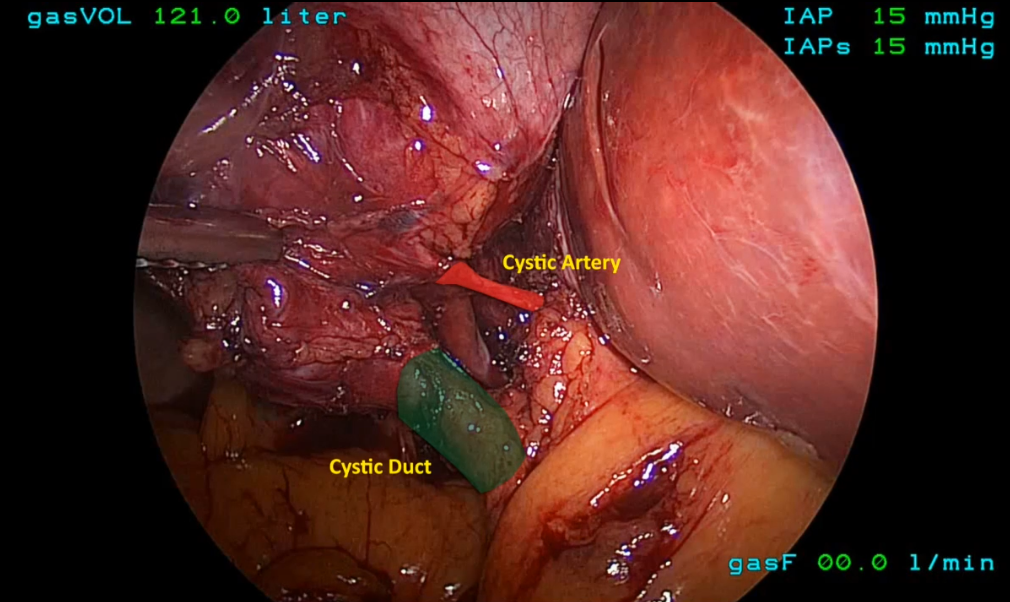
\includegraphics[width=0.6\textwidth]{introduction/img/critical_view_of_safety.png}
    \caption{The critical view of safety. The cystic artery is indicated in red, the cystic duct in green. Image provided with courtesy of~\cite{ALES5766}. Refers to \secref{in:sec:cholecystectomy_procedure}.}
    \label{fig:enter-label}
\end{figure}

\subsubsection{Step 3: Clipping and Cutting the Cystic Artery} After establishing the critical view of safety, the next step is to separate the gallbladder from the cystic artery. Therefore, the csytic artery is clipped twice proximally (i.e. the side of the artery that stays inside the body) and once distally (i.e. on the side of the to be removed gallbladder). The distal clip should be attached close to the neck of the gallbladder to leave sufficient space for cutting. Next, the artery is cut with hook scissors, leaving some space at the proximal end to prevent the clip from detaching.

\subsubsection{Step 4: Operative Cholangiography and Cutting the Cystic Duct} Post cutting the cystic artery, it is sometimes preferred to perform cholangiography, using the C-arm X-ray, which is shown in \figref{in:fig:room_setup}. This is to verify a functioning bile tree. First, the cystic duct is clipped distally, and then incised partially with hook scissors. Next, the common bile duct is flushed with saline and a contrast agent is injected. Fluoroscopy should reveal free flow of the contrast agent into the common hepactic bile duct, its left and right branches into the liver, as well as free flow into the duodenum via the common bile duct. Once satisfactory flow is observed, the cystic duct is clipped proximally and cut as the cystic artery in step three.

% also refer to \secref{in:sec:cholecystectomy_setup}
% ERCP: https://www.sages.org/publications/patient-information/patient-information-for-ercp-endoscopic-retrograde-cholangio-pancreatography-from-sages/

\subsubsection{Step 5: Separating Gallbladder from Liver} After cutting the cystic duct, the gallbladder is carefully dissected from the liver bed, commonly using an L-hook with monopolar energy. Care must be taken to prevent liver bed injury as this may cause bleeding and or bile leakage from superficial ducts. Entry into the gallbladder should be avoided as this may cause bile and bile stone leakage, which, however, can be removed with a suction irrigator, as shown in \figref{in:sec:cholecystectomy_setup}. In complex conditions with gallbladder inflammation, an ultrasound-driven harmonic scalpel may be used to perform ultrasonic coagulation to maintain hemostasis (blood thickening). Finally, the liver bed is once more inspected before separating the gallbladder fully. The surgical side is once more irrigated and cleaned of any blood and bile. The gallbladder is then put into a specimen bag.

\subsubsection{Step 6: Removing Specimen and Closing} Once in a bag, the gallbladder is removed through the T1 port, refer to \figref{in:fig:cholecystectomy_incisions}. This may require widening of the opening in the presence of larger stones. The ports T1-T4 are being vented to remove residual $\text{CO}_2$. Following that, the skin and fascia at the extraction site are closed with sutures.

\section{Robot Assisted Laparoscopy}
\label{in:sec:robot_assisted_laparoscopy}
Having a good understanding of laparoscopic surgery from the previous \secref{in:sec:laparoscopy}, and more specifically, laparoscopic cholecystectomy, we will next discuss robot assisted laparoscopic surgery. We will initially explain the, at first glance, paradoxical rise of robot assisted laparoscopy in \secref{in:sec:the_rise_of_robot_assisted_laparoscopy}. Next, current commercial systems will be analyzed in \secref{in:sec:robot_surgery_platforms}, as to better understand where the field might be headed so to provide an informed research direction. Finally, based on the knowledge of the previous sections, the enhancement of current systems will be discussed in \secref{in:sec:enhancing_current_systems}.

\subsection{The Rise of Robot Assisted Laparoscopy}
\label{in:sec:the_rise_of_robot_assisted_laparoscopy}
According to many, the future of surgery is robotic~\cite{times2021better}. This trend was already exposed in \secref{in:sec:foreword}, \figref{in:fig:robotic_vs_laparoscopic_vs_open}, where~\cite{sheetz2020trends} found an average increase in robotic laparoscopy from $1.8\%$ to $15.1\%$ post robotic laparoscopy introduction. For cholecystectomy, the most common procedure, an increase from $2.5\%$ to $7.5\%$ was found. Somewhat paradoxically, (non-robotic) laparoscopic cholecystectomy is already a routine procedure with very low complication rates,~\cite{thapar2023evaluation} e.g. reports a $0.2\%$ 30 days mortality rate in India. Hence, questions about benefits of robotic laparoscopy may rightfully be raised.

\paragraph{Patient Side Aspects} More than twenty years have passed since the introduction of the da Vinci\textsuperscript{\textregistered} surgical robot by Intuitive (\figref{in:fig:da_vinci}), which was launched in 1999, and many review studies compared classical vs. robotic laparoscopies ever since to provide evidence-based care. The majority of studies suggests that no significant advantages exist for patients. Despite increased cost and longer intervention times, these studies report equal complication, mortality, and conversion rates (i.e. conversion to open surgery), as well as equal post operative stay duration~\cite{kawka2023laparoscopic, csirzo2023robot}. Some studies, however, also highlight underrepresented patient-reported outcome measures~\cite{kawka2023laparoscopic} (e.g. post-operative pain, return to function). 

\paragraph{Surgeon Side Aspects} Undoubtedly, the market for \gls{ras}, which is currently dominated by Intuitive Surgical, Inc., is sustainably growing. 

%, see \figref{in:fig:intuitive_revenue}.
\begin{figure}[tb]
    \centering
    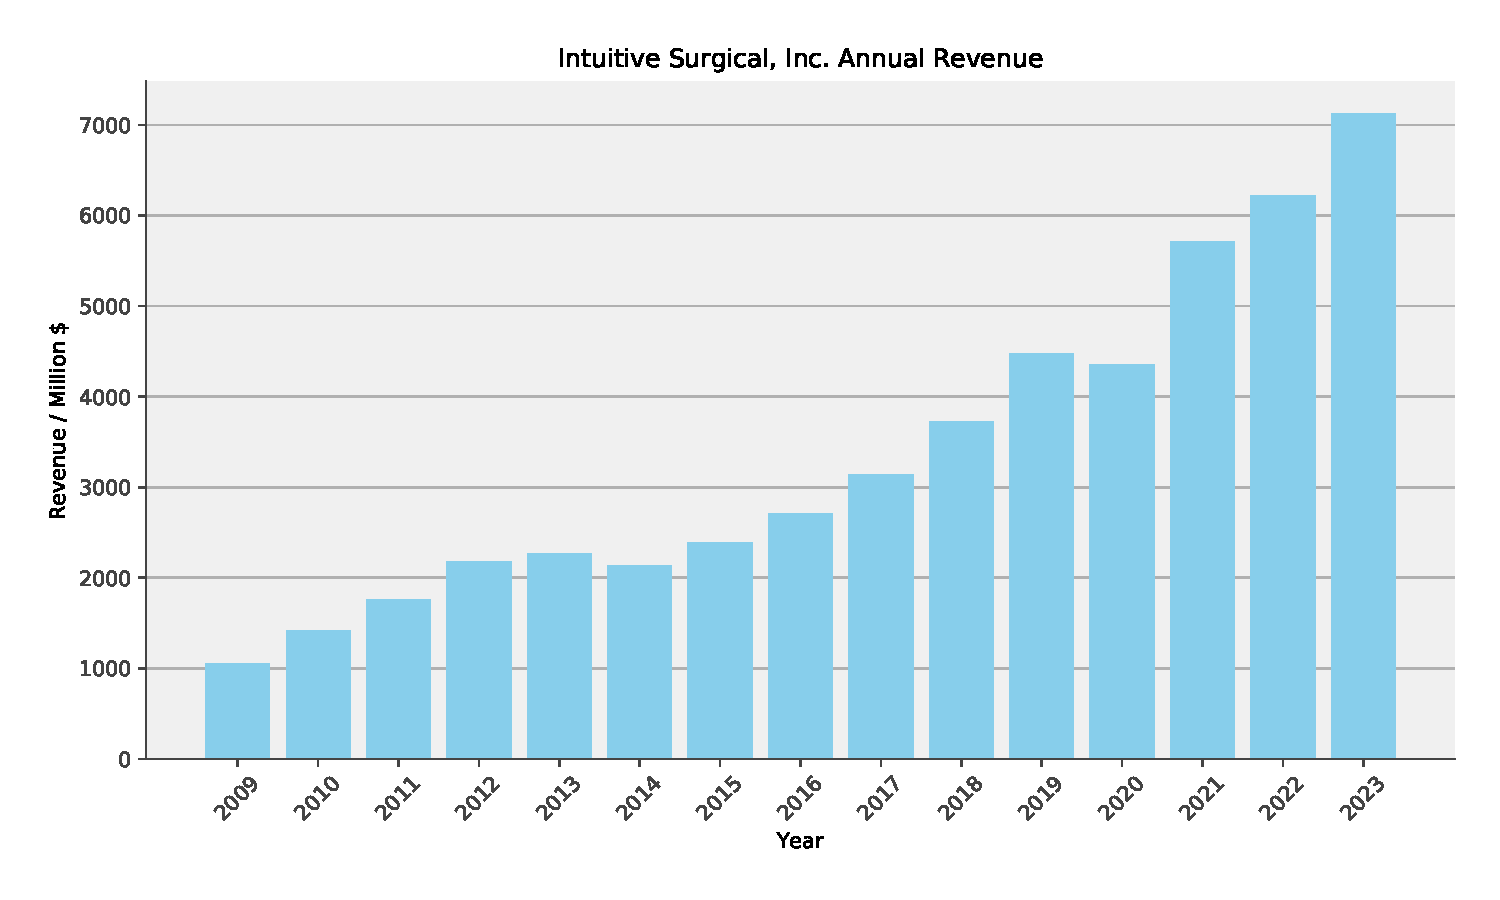
\includegraphics[width=0.9\textwidth]{introduction/fig/intuitive_revenue.pdf}
    \caption{Annual revenue of Intuitive Surgical, Inc. from 2009 to 2023. The company has achieved sustained growth throughout the years. Data obtained from~\cite{intuitiverevenue}.}
    \label{in:fig:intuitive_revenue}
\end{figure}

The reasons for this steady growth, as per above and to the best current knowledge, cannot be associated with patient benefits. Instead, the growth can be linked to surgeon benefits. Multiple studies suggest ergonomic advantages for surgeons~\cite{monfared2022comparison, zarate2019ergonomic}, which prevent operating burnout~\cite{wells2019operating} and improve longevity~\cite{stucky2018surgeon}. This evidence can best be understood through the surgery that lead to the initial success of the da Vinci\textsuperscript{\textregistered} surgical robot, the minimally invasive prostatectomy. The prostate, being located low (inferiorly) in the pelvis, is hardly accessible via laparoscopic tools. The large distance from trocar to prostate makes precise motion difficult and creates a lever that generates torques which cause fatigue. A robot makes it ergonomically much simpler to operate in these areas. In England, about $85\%$ of radical prostatectomies in $2017$ were performed robotically~\cite{maynou2021patterns}.

\paragraph{Interviewing a Surgeon} To find further qualitative insights on the advantages of \gls{rmis} over \gls{mis}, we interviewed Nicholas Raison, a consultant urological surgeon, during a course he organized for robotic partial nephrectomy, hosted by the International Medical Robotics Academy at Guy's Hospital \gls{kcl}. Among the aforementioned lever with associated fatigue reduction, and precision improvements, he named four more advantages of robotic platforms. First, classical laparoscopic tools are straight and do not allow for wrist rotations at the grippers. Robotic tools provide additional degrees of freedom and therefore increased dexterity. This simplifies tasks such as suturing significantly. Second, the control of the tools through a console allows the surgeon to operate from a first-person view which reduces mental burden. Third, \gls{rmis} reduces the learning curve for newly trained surgeons, which results from the enhanced dexterity and the first-person view.
Finally, since surgeons are in charge of moving the camera themselves in \gls{rmis}, they tend to move it more frequently which provides them with a precise view. In classical \gls{mis}, there exists a communication barrier with the camera holder, refer \figref{in:fig:room_setup}. Therefore, in classical \gls{mis}, camera holders sometimes show a distant view to compensate for this communication barrier. This last point highlights the potential value of endoscope motion automation, enabling a future fusion of \gls{rmis} and \gls{mis} techniques. 

\paragraph{Future Aspects} In summary, and to best current evidence, robotic surgery platforms currently do not provide  improved surgery outcomes, but increase operating cost and time. Viewed differently, they don't worsen the surgery outcomes either. What makes robotic laparoscopy so successful are the surgeon side benefits and its future prospects. These e.g. include the possibility to control the systems remotely, data collection, realistic simulations for training, and potential automation. With this in mind, the research carried out in this thesis aims to address the increased cost and  time components, emphasizing on laparoscopic camera motion automation. To get a better understanding for how this could best be achieved, the next section provides an overview of current robot surgery platforms.

% ⁃	Versius jerky, less smooth, no rotation about entry axis
% ⁃	Hugo better range of motion inside abdomen vs xi
% ⁃	Xi console restricting (goggles)
% ⁃	Hugo console open 
% ⁃	Versius console no foot pedals 
% ⁃	Versius common laparoscopic tools, cheaper but less versatile
% ⁃	Much more camera motion in robotic surgery compared to classic laparoscopic surgery (surgeons adjust to their desired view more commonly. Camera in traditional surgery further away to correct for communication shortcoming)
% ⁃	Ergonomic benefits in robotic surgery (large lever over entry point, generating lots of torque)
% ⁃	Versius small company in comparison to pharmaceutical giants 
% ⁃	Footprint xi surprisingly small 
% ⁃	Da Vinci console weight engaged, Hugo head tracking engaged (tracks glasses via camera and infrared balls on glasses)
% ⁃	Hugo console feels laggy compared to da Vinci 
% ⁃	Classical laparoscopic tools are straight, robotic tools offer additional dof, making e.g. suturing much simpler
% ⁃	Da Vinci arm arm collisions happen, in which case the assistant attempts to readjust the configuration 
% ⁃	Versius changes tools via joystick, whereas other systems can change arm via footpedals
% ⁃	Proximie providing views of the da Vinci during live stream 

\subsection{Robot Surgery Platforms}
\label{in:sec:robot_surgery_platforms}
\begin{figure}[tb]
    \centering
    \begin{subfigure}[b]{0.49\textwidth}
        \centering
        \includegraphics[width=\textwidth]{introduction/img/JPG_Large-DV_SYS_Xi_PatientCart_PRF_RGB-min.jpg}
        \caption{The da Vinci\textsuperscript{\textregistered} Xi system. Images provided with courtesy of \textcopyright2023 Intuitive Surgical Operations, Inc.}
        \label{in:fig:da_vinci}
    \end{subfigure}
    \begin{subfigure}[b]{0.49\textwidth}
        \centering
        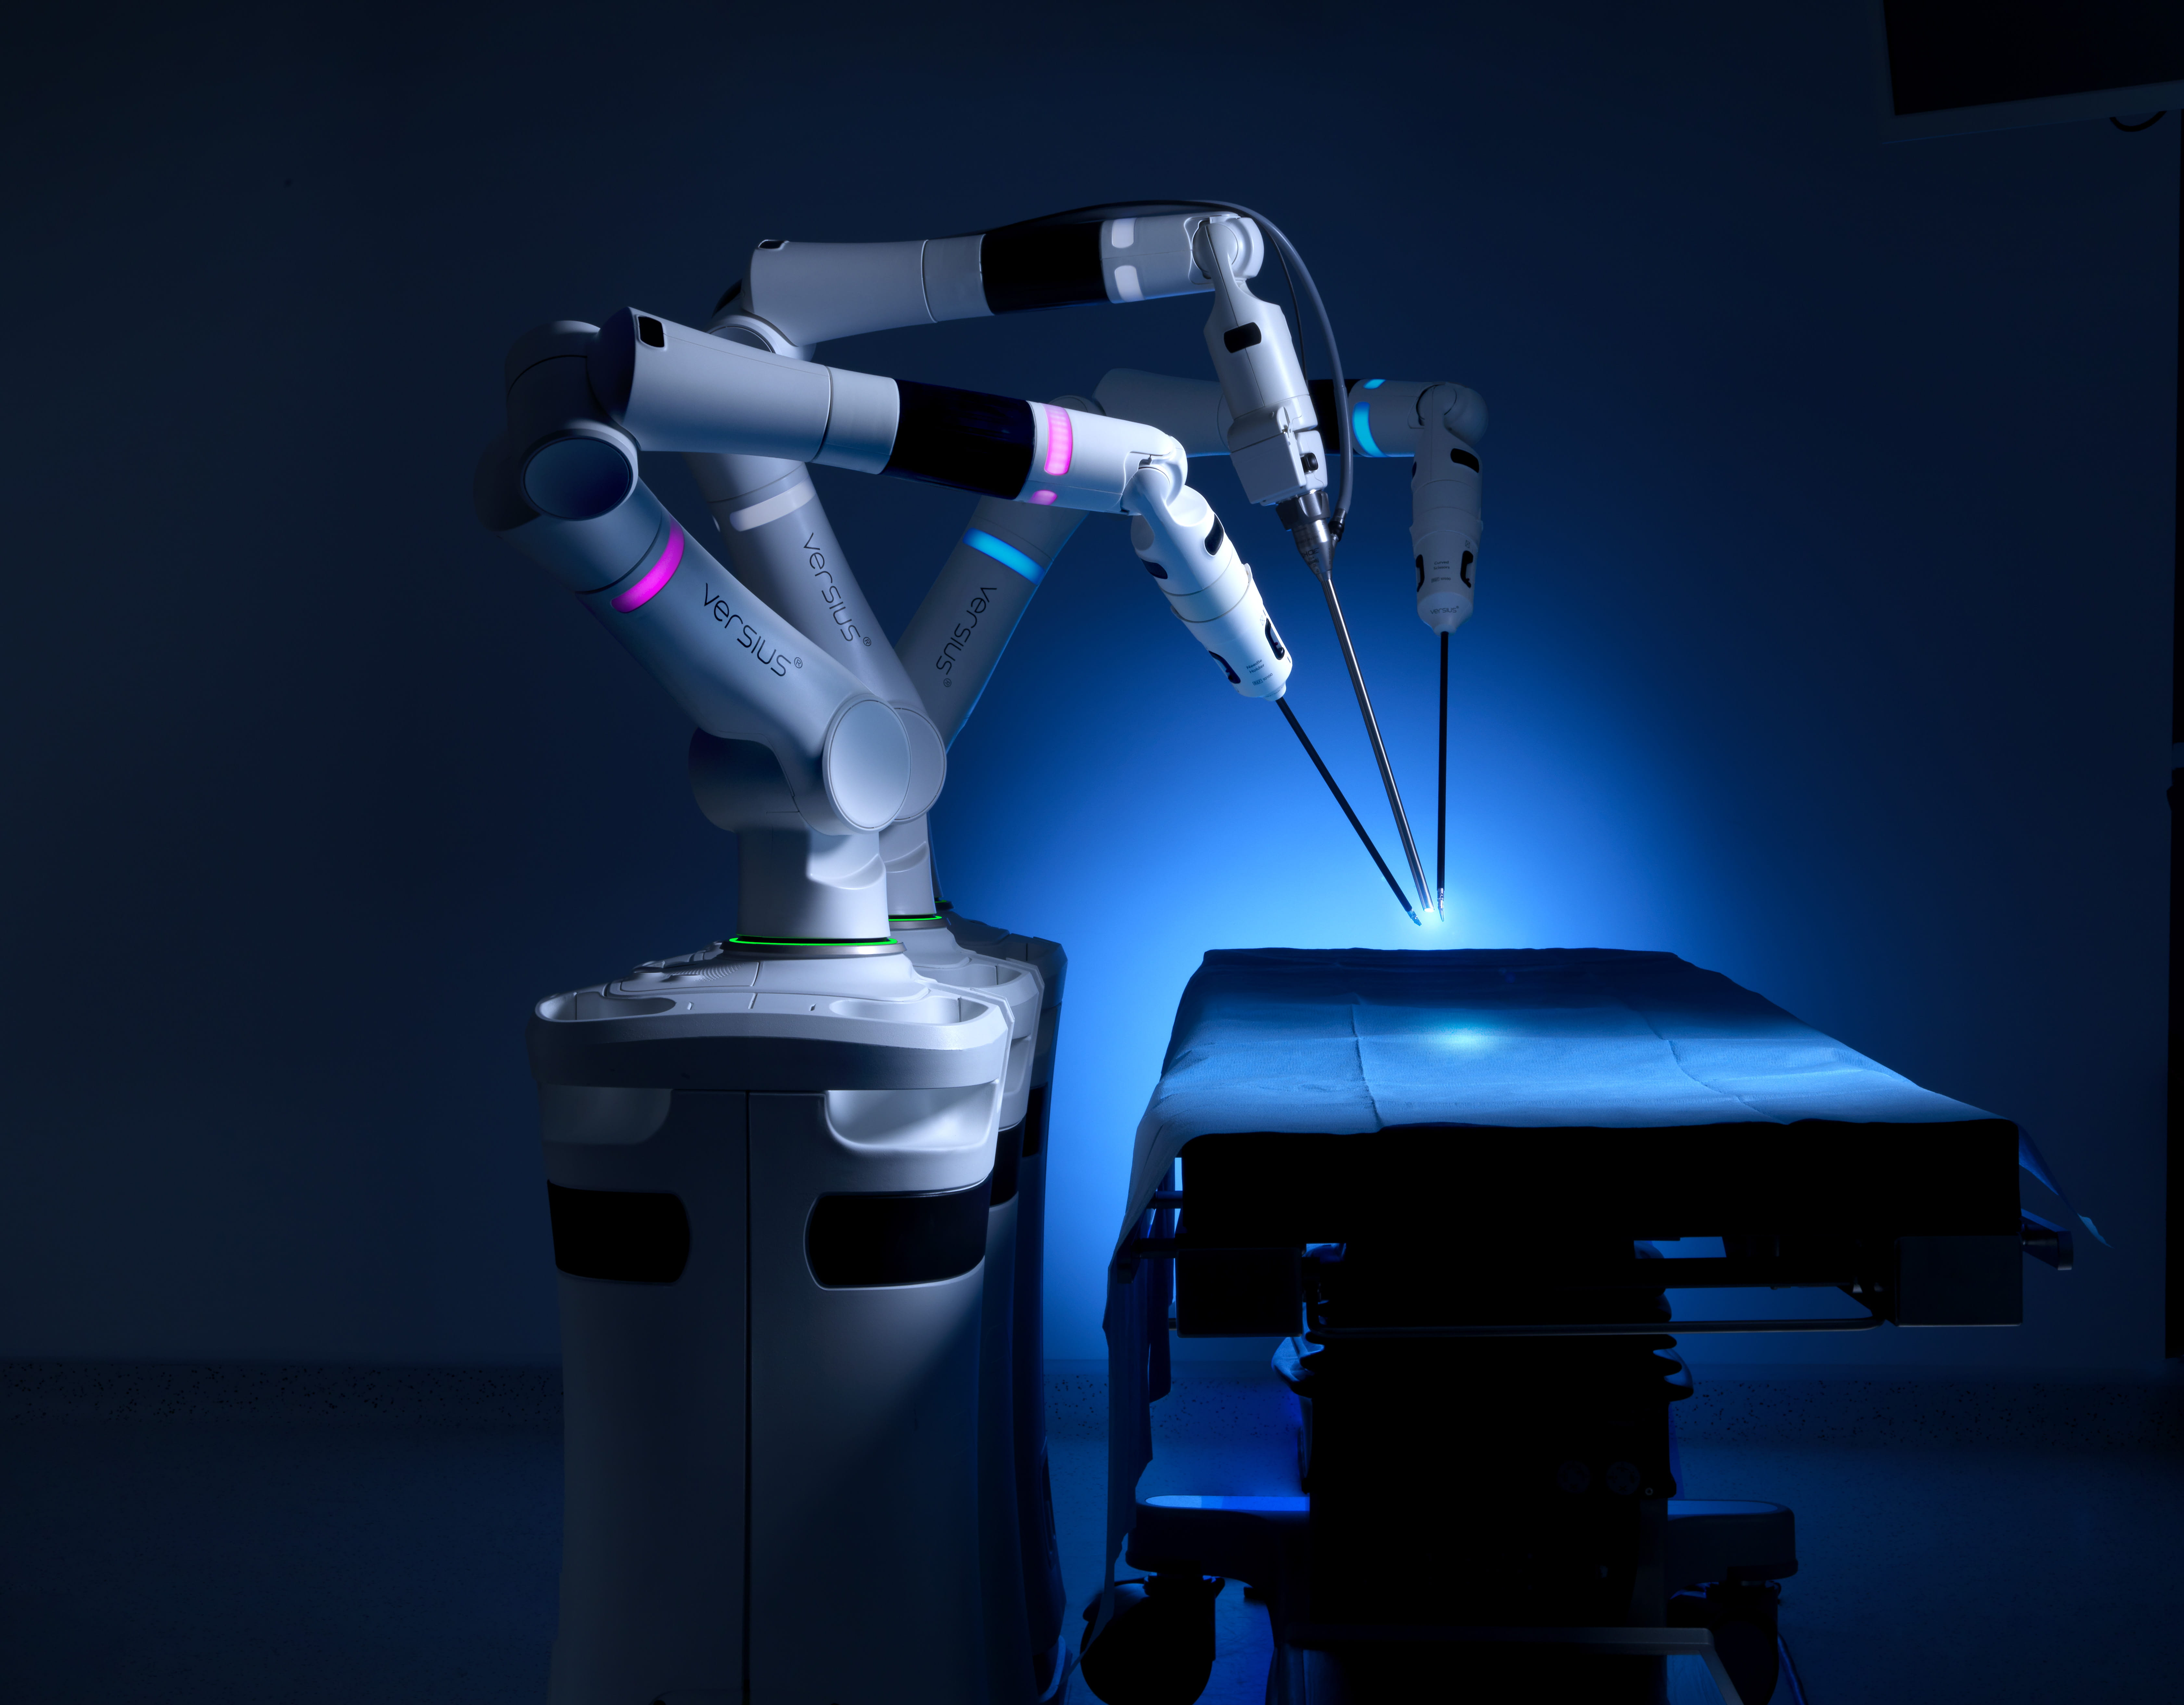
\includegraphics[width=\textwidth]{introduction/img/Product-Versius-3-Arm-Setup-B.jpg}
        \caption{The Versius\textsuperscript{\textregistered} system. Images provided with courtesy of \textcopyright2023 \gls{cmr} Surgical, Ltd.}
        \label{in:fig:versius}
    \end{subfigure}
    \caption{Two examples of currently available commercial robotic laparoscopy systems. It is demonstrated how competition has led to two very different designs. The da Vinci\textsuperscript{\textregistered} Xi system in \figref{in:fig:da_vinci} is monolithic with a mechanical \gls{rcm}. The Versius\textsuperscript{\textregistered} system is modular with a programmable \gls{rcm}. Refers to \secref{in:sec:robot_surgery_platforms}.}
    \label{in:fig:surgical_systems}
\end{figure}

The da Vinci\textsuperscript{\textregistered} robot by Intuitive (\figref{in:fig:da_vinci}) was launched in 1999 by Intuitive Surgical, Inc., which filed multiple patents in the 1990s thereby guarding market access from other companies. Patents in the US generally last for 20 years, which is why as of 2020 most of these critical patents have ran out. Many other companies are now trying to gain some of Intuitive's market share. This competition will ultimately benefit patients, as it might help drive down cost for robotic surgery in the future~\cite{patel2021can}, increase accessibility, and lead to innovation in general. 

A non-exhaustive overview of current commercial systems is given in \tabref{in:tab:systems}. It can be seen that the competition has already brought innovation and a broader variety of systems. Multiple companies are adopting Intuitive's monolithic structure, that is all robotic arms are attached to a single instance. Many others, such as Medtronic and \gls{cmr} Surgical, are taking a modular approach instead. The systems further differentiate themselves not only by their modularity, but also through their mechanical properties. The da Vinci\textsuperscript{\textregistered} robot has a mechanical remote center of motion (\gls{rcm}), i.e. there are dedicated \gls{dof} for achieving a zero translational velocity at the entry point to the patient. The \gls{rcm} is also sometimes called fulcrum point in the medical context. Having a mechanical \gls{rcm} provides additional safety, but leads to systems that are hard to re-purpose. This is why recent systems are exploring programmable \gls{rcm}s, in which a \gls{rcm} is achieved through control theory. This has implications on safety, as sometimes the \gls{rcm} may not be achieved, but can potentially provide multi-purpose systems. 

\begin{table}[tb]
\centering
\caption{A non-exhaustive list of commercial robotic laparoscopy systems. The table differentiates between monolithic / modular systems and systems with mechanical / programmable \gls{rcm}. The market competition has lead to a variety of systems with a tendency to stand apart from Intuitive's status-quo approach. Refers to \secref{in:sec:robot_surgery_platforms}.}
\label{in:tab:systems}
\begin{tabular}{lll}
                                       & Mechanical \gls{rcm}                                                                                                                                                                                                                                                                                                             & Programmable \gls{rcm}                                                                                                                                                                                                                                                                                                         \\ \cline{2-3} 
\multicolumn{1}{l|}{Monolithic} & \multicolumn{1}{l|}{\begin{tabular}[c]{@{}l@{}}$\bullet$ da Vinci\textsuperscript{\textregistered} (Intuitive)\\ $\bullet$ Maestro\textsuperscript{\textregistered} (Moon Surgical)\end{tabular}} & \multicolumn{1}{l|}{\begin{tabular}[c]{@{}l@{}}$\bullet$ hinotori\textsuperscript{\texttrademark} (Medicaroid)\\ $\,$\end{tabular}}                                                                                                                                                            \\ \cline{2-3} 
\multicolumn{1}{l|}{Modular}    & \multicolumn{1}{l|}{\begin{tabular}[c]{@{}l@{}}$\bullet$ Hugo\textsuperscript{\texttrademark} (Medtronic)\\ $\bullet$ SSi Mantra\textsuperscript{\texttrademark} (SS Innovations)\\ $\,$\end{tabular}}                                                                                  & \multicolumn{1}{l|}{\begin{tabular}[c]{@{}l@{}}$\bullet$ Versius\textsuperscript{\textregistered} (\gls{cmr} Surgical)\\ $\bullet$ Dexter\textsuperscript{\textregistered} (Distalmotion)\\ $\bullet$ Senhance\textsuperscript{\texttrademark} (Asensus Surgical)\end{tabular}} \\ \cline{2-3} 
\end{tabular}
\end{table}

\subsection{Enhancing Current Systems}
\label{in:sec:enhancing_current_systems}
The previous two sections gave an explanation for the rise of robot assisted laparoscopy in \secref{in:sec:the_rise_of_robot_assisted_laparoscopy}, and introduced different commercial systems in \secref{in:sec:robot_surgery_platforms}. We identified surgeon side benefits as well as future prospects as the main driving factors for \gls{rmis}. Adoption is, however, slowed down by roadblocks such as surgery cost, about $\$1000-4000$ of additional cost per procedure~\cite{neumann2018qalys}, and additional operation time, about $25$ minutes of additional operation time for cholecystectomy (185 vs 160 minutes~\cite{kane2020robotic}). Patient outcomes are just as good in \gls{rmis} as they are in \gls{mis}. This is to be expected as patient outcomes for \gls{mis} are already much better than for open surgery and the bar for further improvement is high. Consequentially, patient outcomes cannot be considered a limitation of current systems and are thus not of immediate relevance for research. Now, to enhance current systems, we argue that it is most efficient to work on the driving factors that made \gls{rmis} successful in the first place, as well as the roadblocks. The overarching goal of this thesis, laparoscopic camera motion automation, fits nicely into the clinically relevant enablers and challenges for \gls{rmis}, as shown in \figref{in:fig:advancing_robotic_laparoscopy}. A prerequisite for automating a robotic system in a \gls{phri} environment, however, is spatial awareness. Spatial awareness comes with the additional benefit that it also contributes to operation time and surgeon convenience, as will be described in the next section.
\begin{figure}[tb]
    \centering
    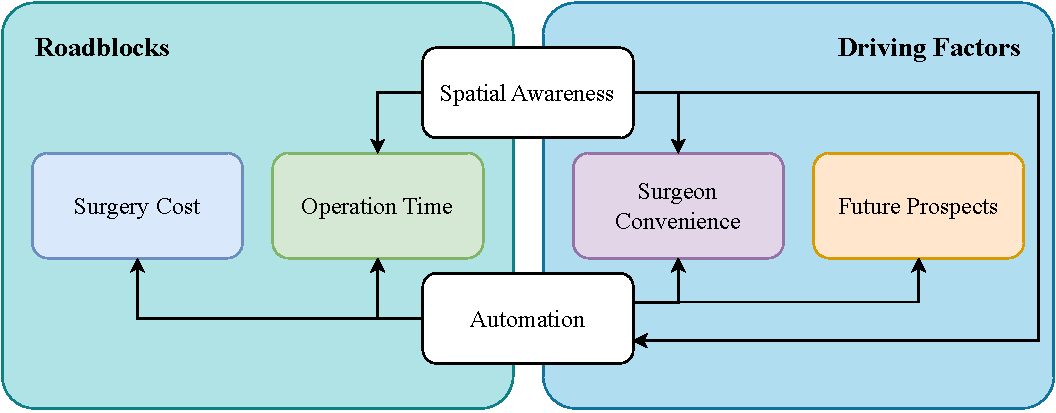
\includegraphics[width=\textwidth]{introduction/fig/main_goals.pdf}
    \caption{Roadblocks and driving factors of \gls{rmis} and how the targets of this thesis, spatial awareness and automation, alleviate and enhance them, respectively, refers to \secref{in:sec:enhancing_current_systems}.}
    \label{in:fig:advancing_robotic_laparoscopy}
\end{figure}

\subsubsection{Spatial Awareness}
\label{in:sec:spatial_awareness}
Spatial awareness is likely the most underexplored domain in \gls{rmis}. By spatial awareness we will be referring to highly precise localization necessary for surgery, that is in the order of $1\,\text{cm}$ or less. In the cluttered operating theater, containing an anesthesia machine, monitors, a C-arm, staff, the patient, the surgeon, and many other devices, refer \figref{in:fig:room_setup}, collisions are inevitable. A staggering amount of 5 arm-arm, and or assistant-arm collisions occur on average in robotic colorectal surgery~\cite{wong2023improving}. Pain or bruising from hindrance by the robot arm is reported by $20\%$ of assistants ~\cite{van2019ergonomic}. Training assistants could mitigate some of these issues, which, as many studies imply~\cite{cimen2019does, mitsinikos2017does, kwon2020impact}, would lead to improved performance, and therefore, surgeon convenience and operation time reduction. 

To this end, we argue differently and assign the responsibility to the robotic system rather than the assistants or surgeons. These highly capable robotic systems should prevent collisions themselves and leave the clinical workflow unaltered. Some works suggest image-based avoidance~\cite{hameed2016towards} and 3D avoidance~\cite{li2023three}, both of which could benefit from spatial awareness. Collision avoidance might even become more relevant with the adoption of modular systems, as outlined in \secref{in:sec:robot_surgery_platforms}. Spatial awareness would not only improve performance by reducing collisions, it would further contribute to workspace optimization works, such as~\cite{hutzl2015knowledge, zelechowski2023automatic}, as these require accurate knowledge about the relative patient-robot position. Workspace optimization is not only crucial from a robotic point of view but for clinical aspects as well~\cite{alhusseinawi2023validation}. As such, recent studies highlight that it takes an average of $18$ minutes to perform proper docking in robotic adrenalectomy~\cite{feng2020robot}.

\subsubsection{Automation}
\label{in:sec:automation}
As already outlined in the foreword \secref{in:sec:foreword}, laparoscopic camera motion automation is likely the first milestone towards automated \gls{rmis}. The short-term benefits of automation are less obvious than for improved spatial awareness, which was explained above, however, the long-term benefits and thus the future prospects justify investigation. Automation, shown in \figref{in:fig:advancing_robotic_laparoscopy}, could e.g. have positive implications on surgery cost, operation time, surgeon convenience.

% Automation in robot-assisted minimally invasive surgery (RMIS) may reduce human error that is linked to fatigue, lack of attention and cognitive overload~\cite{fiorini2022concepts}.
%It could help surgeons operate such systems by reducing the learning curve~\cite{van2018learning}.
%And in an ageing society with shrinking workforce, it could help to retain accessibility to healthcare. It is therefore expected that parts of \gls{rmis} will be ultimately automated~\cite{davenport2019potential,zidane2022robotics}.

Some works argue that automation may reduce human error that is linked to fatigue, lack of attention and cognitive overload~\cite{fiorini2022concepts}, therefore contribute to operation time and surgeon convenience. Similarly, automation could help surgeons operate robotic systems by reducing the learning curve~\cite{van2018learning}. On a societal scale, and in an ageing society with shrinking workforce, automation could help to retain accessibility to healthcare and limit cost. This could e.g. be achieved through digital twins of surgeons~\cite{zidane2023robotics} (CEO of Asensus Surgical, Senhance\textsuperscript{\texttrademark} surgical robot). It is, therefore, expected that parts of \gls{rmis} will be ultimately automated~\cite{davenport2019potential,zidane2022robotics}.

In this work, and as will be discussed in the following paragraphs, we will be looking at concrete advantages of automation, like continuous camera motion, as well as strategies that are to be taken into consideration for successful automation of camera motion in laparoscopic surgery.

% creates uncertainties and ethical and legal issues

\paragraph{Continuous Camera Motion} Current \gls{rmis} systems, like the da Vinci\textsuperscript{\textregistered} or the Hugo\textsuperscript{\texttrademark} robots, strictly separate camera and tool motion to prevent collisions. This separation helps to remove some mental burden from the surgeon, however, lowers the efficiency and increases the operation time, which in turn has implications on the surgery cost. Having to switch constantly between camera and tool motion also introduces inconvenience to the surgeon. Camera motion automation could help alleviate all these by introducing continuous camera motion. In fact, and as explained in \secref{in:sec:the_rise_of_robot_assisted_laparoscopy} - Interviewing a Surgeon, \gls{rmis} already leads to more frequent camera motion when compared to \gls{mis}. It is therefore expected that even more camera motion is desirable for surgeons.

\paragraph{Robot-free Surgeries} Surgery cost might not only be reduced through continuous camera motion, it might also be reduced in procedures where robot assistance is currently not common practise, such as laparoscopic cholecystectomy. In Michigan, United States, e.g., only $7.5\%$ of all laparoscopic cholecystectomies were performed with a robot~\cite{sheetz2020trends}. The numbers are likely lower in other countries. Domains without robot dominance could initially benefit from replacing the camera holder assistant, refer \figref{in:fig:room_setup}, thus reducing the cost drastically and also allowing the assistant to perform more meaningful tasks. This could further remove the communication barrier between surgeon and camera holder, therefore improving the surgeon convenience and reducing the operation time. 

Indeed, some companies, e.g. Moon Surgical (Maestro\textsuperscript{\textregistered}), \gls{cmr} Surgical (Versius\textsuperscript{\textregistered}), and Distalmotion (Dexter\textsuperscript{\textregistered}), target this area through their modular systems, even if they are not introducing automation yet. Due to the progressive nature of healthcare~\cite{chatterjee2024advancements}, it is almost certain that automation will grow in importance as robots will be deployed to laparoscopic cholecystectomy. Automating camera motion in domains without robot dominance introduces implications that will become clearer in \secref{in:sec:imitation_learning}. We hold that any laparoscopic camera motion automation attempt should be compatible with surgeries that are robotic and those that will be robotic or hybrid.



% so why does automation contribute to 
% - surgery cost (camera holder)
% - operation time (camera motion separation)
% - surgeon convenience (fatigue, learning curve, attention)
% - future prospects (lack of staff, etc, better accesibility through standardization)

% trend towards progress in healthcare:~\cite{chatterjee2024advancements}


\paragraph{System Considerations} Whilst automation can be achieved on robotic systems with mechanical \gls{rcm} and systems with programmable \gls{rcm}, refer \secref{in:sec:robot_surgery_platforms}, in this work, the main focus will be put on systems with programmable \gls{rcm}. This is inline with our belief that modular systems will increase their market share, as well as the availability of experimental platforms of relevance. Systems with programmable \gls{rcm} can be used flexibly across multiple types of surgeries, e.g. spine~\cite{farber2021robotics} or orthopaedic surgery~\cite{suarez2023revolutionizing}, thereby reducing cost even more. To facilitate the potential cost reduction that arise with programmable \gls{rcm}s, methods in this thesis should therefore not be limited to, but also obey the principles of programmable \gls{rcm}s. 


% In summary and what is important for us: Programmable \gls{rcm}, domains without robot dominance, a lot of this reasoning stems from economics and growth


% Now, specifics for automation will further be discussed in \secref{in:sec:camera_motion_automation}


% name some clinical aspects for why automation is important, learning curve, lack of staff, fatigue, attention etc







% da vinci system review~\cite{ngu2017vinci}
% Without impacting clinical workflow
% Whilst current commercial systems are quite capable already 
% explain limitations of current systems, missed opportunities given current robots (capable actuators)

\section{Spatial Awareness in Robotic Laparoscopy}
\label{in:sec:spatial_awareness_in_robotic_laparoscopy} 

The previous \secref{in:sec:enhancing_current_systems} outlined the need for improved spatial awareness in robotic laparoscopy, i.e. knowing the robot's and the laparoscope's locations. It is a prerequisite for automation and facilitates improved clinical workflow for reduced surgery time and surgeon convenience but also adds clinically relevant workspace knowledge. Since we are interested in adding spatial awareness through low cost sensors, i.e. cameras, in this section we will initially summarize camera intrinsic parameter calibration in \secref{in:sec:camera_intrinsic_calibration}, which is a prerequisite for all that follows. Then, the concepts of eye-in-hand and eye-to-hand calibration are discussed in \secref{in:sec:eye_in_to_hand}, see \figref{in:fig:coordinate_frames}. Next, we will evaluate the clinical workflow implications for these types of calibrations in \secref{in:sec:unified_calibration}, and finally we will propose novel methods for marker-free calibration that leave the clinical workflow vastly unaltered in \secref{in:sec:unified_calibration}.
\label{in:sec:eye_in_to_hand}

\begin{figure}[tb]
    \centering
    \begin{subfigure}[b]{0.49\textwidth}
        \centering
        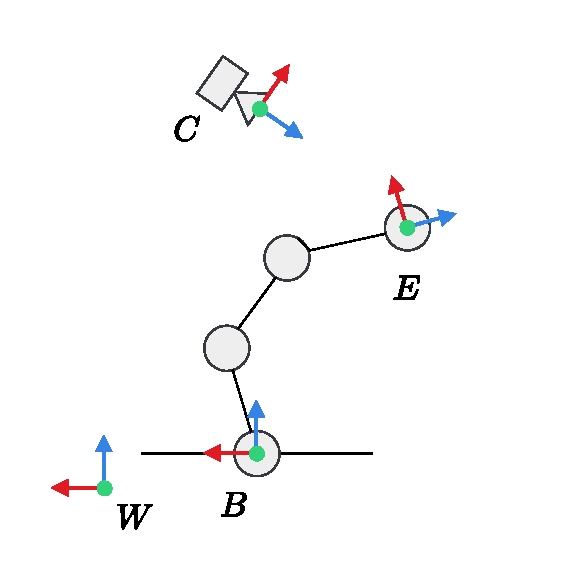
\includegraphics[width=\textwidth]{introduction/fig/eye_to_hand.pdf}
        \caption{Eye-to-hand setup.}
        \label{in:fig:eye_to_hand}
    \end{subfigure}
    \begin{subfigure}[b]{0.49\textwidth}
        \centering
        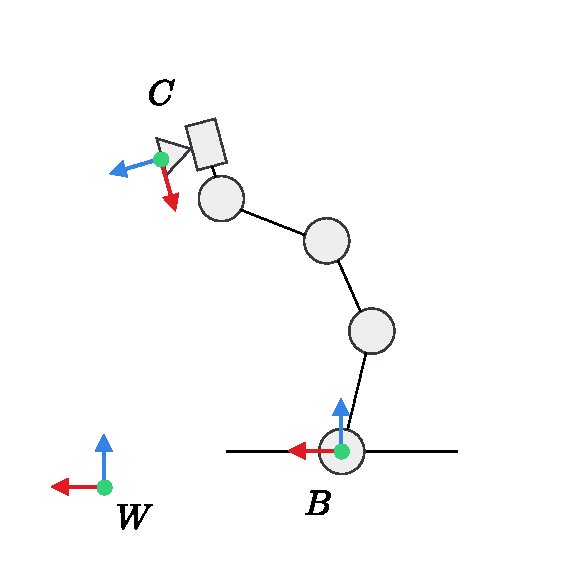
\includegraphics[width=\textwidth]{introduction/fig/eye_in_hand.pdf}
        \caption{Eye-in-hand setup.}
        \label{in:fig:eye_in_hand}
    \end{subfigure}
    % 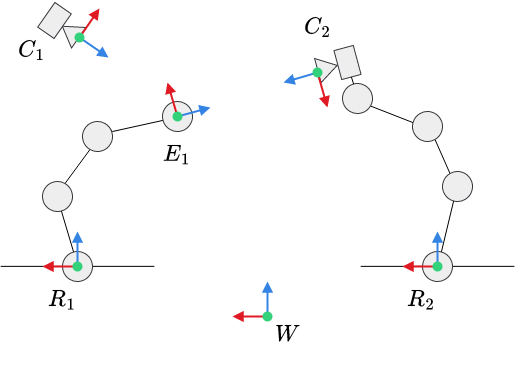
\includegraphics[width=\textwidth]{introduction/fig/eye_in_to_hand.png}
    \caption{Eye-to-hand, and eye-in-hand setups for serial arm manipulators. Camera frames $C$, robot base frame $B$, end-effector frame $E$ and world frame $W$. Real setups might consist of multiple robots. Refers to \secref{in:sec:spatial_awareness_in_robotic_laparoscopy}.}
    \label{in:fig:coordinate_frames}
\end{figure}

\subsection{Camera Intrinsic Parameter Calibration}
\label{in:sec:camera_intrinsic_calibration}
Camera intrinsic parameters describe how 3D points are projected onto the observed 2D image plane. This image formation process is crucial for relating 3D points to 2D observations and vice-versa. Let $p_{_W}$ be a 3D point expressed in homogeneous coordinates with respect to the world frame $W$, $p_{_W} = \begin{bmatrix}
    x_{_W} & 1
\end{bmatrix}^T$, $x_{_W} = \begin{pmatrix}
    x_{_W} & y_{_W} & z_{_W}
\end{pmatrix}^T$. It is projected into the camera coordinate frame $C$ via a homogeneous transform $\homogeneous{C}{W}$ as

\begin{equation}
    p_{_C} = \homogeneous{C}{W} p_{_W}.
\end{equation}

Under the pinhole camera model, the point $p_{_C}$ is then projected onto the image plane via the intrinsic camera parameters $K$

% e.g. https://docs.opencv.org/4.x/dc/dbb/tutorial_py_calibration.html
% https://docs.opencv.org/4.x/d9/d0c/group__calib3d.html
\begin{equation}
    K = \begin{bmatrix}
        f_x & 0 & c_x \\
        0 & f_y & c_y \\
        0 & 0 & 1 \\
    \end{bmatrix},
\end{equation}

containing the focal lengths $f_{x/y}$, and the principal point $c_{x/y}$. Thus, the observed point in homogeneous image coordinates $u = \begin{pmatrix}
    u & v & 1
\end{pmatrix}^T$ is obtained through

\begin{equation}
    su = K P \homogeneous{C}{W} p_{_W},
\end{equation}

With $P = \begin{bmatrix}
    I^{3\times3} &  0
\end{bmatrix}$, simply being a projection matrix, and $s$ being a scalar usually set to $s = z_{_C}$ when $z_{_C} \neq 0$. Therefore yielding

\begin{equation}
    \begin{bmatrix}
        u \\
        v
    \end{bmatrix} = \begin{bmatrix}
        f_x x_c/z_c + c_x \\
        f_y y_c/z_c + c_y
    \end{bmatrix}.
\end{equation}

This projection assumes perfect optics, which is not the case in general. Real-world optics introduce radial and some tangential distortion. It is for this reason that distortion is accounted for via

\begin{equation}
    \begin{bmatrix}
        u \\
        v
    \end{bmatrix} = \begin{bmatrix}
        f_x x'' + c_x \\
        f_y y'' + c_y
    \end{bmatrix},
\end{equation}

with

\begin{equation}
    \begin{bmatrix}
        x'' \\
        y''
    \end{bmatrix}=\begin{bmatrix}
        x' \frac{1+k_1 r^2+k_2 r^4+k_3 r^6}{1+k_4 r^2+k_5 r^4+k_6 r^6}+2 p_1 x' y'+p_2\left(r^2+2 x^{\prime 2}\right)+s_1 r^2+s_2 r^4 \\
        y' \frac{1+k_1 r^2+k_2 r^4+k_3 r^6}{1+k_4 r^2+k_5 r^4+k_6 r^6}+p_1\left(r^2+2 y^{\prime 2}\right)+2 p_2 x' y'+s_3 r^2+s_4 r^4
    \end{bmatrix},
\end{equation}

\begin{equation}
    r^2 = x'^2 + y'^2,
\end{equation}

and

\begin{equation}
    \begin{bmatrix}
        x' \\
        y'
    \end{bmatrix} = \begin{bmatrix}
        x_c/z_c \\
        y_c/z_c
    \end{bmatrix}.
\end{equation}

Therein, $k_i$ are radial distortion coefficients, $p_i$ tangential distortion coefficients, and $s_i$ then prism coefficients. A camera calibration is performed through observing a pattern of known dimensions, e.g. a checkerboard, from various angles and positions, and optimizing for the model parameters, i.e. camera intrinsic parameters and distortion coefficients, such that the known projected points equal the observed and undistorted points.

\subsection{Eye-in-hand and Eye-to-hand Calibration}
\label{in:sec:eye_in_to_hand_calibration}
An overview of eye-in-hand and eye-to-hand setups is shown in \figref{in:fig:coordinate_frames}. Eye-in-hand calibration refers to the process of finding the camera frame $C$ to robot end-effector frame $E$ transformation $\homogeneous{E}{C}$ when the camera is attached to the robot's end-effector. Eye-to-hand calibration refers to finding the camera frame $C$ to robot base frame $B$ transformation $\homogeneous{B}{C}$ when the camera is statically placed next to the robot. A prerequisite for this type of calibration is a well known camera model, as was described in \secref{in:sec:camera_intrinsic_calibration}.

The calibration is performed by collecting target to camera $\homogeneous{T}{C}$ and robot base to end-effector transformations $\homogeneous{E}{B}$. Given undistorted camera images, and the camera intrinsic parameters, refer \secref{in:sec:camera_intrinsic_calibration}, target to camera transforms $\homogeneous{T}{C}$ can e.g. be obtained through solving a \gls{pnp} problem, where points are commonly obtained through ArUco markers, see \figref{in:fig:eye_in_hand_setup}. The base to end-effector transformation $\homogeneous{E}{B}$ can be obtained through robot kinematics.
\begin{figure}[htb]
    \centering
    \begin{subfigure}[b]{0.49\textwidth}
        \centering
        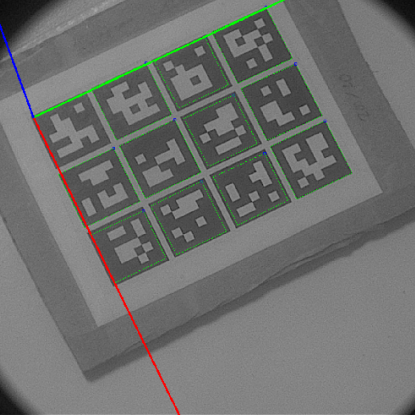
\includegraphics[width=\textwidth]{introduction/img/aruco.png}
        \caption{Undistorted exoscope view of the ArUco marker target.}
    \end{subfigure}
    \begin{subfigure}[b]{0.49\textwidth}
        \centering
        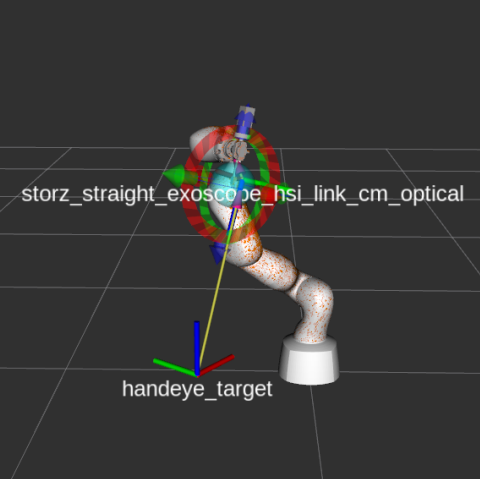
\includegraphics[width=\textwidth]{introduction/img/aruco_world.png}
        \caption{Mesh visualization of robot state with estimated camera and target poses.}
    \end{subfigure}
    \caption{Eye-in-hand calibration example in a realistic scenario. Used hardware includes: Storz VITOM Telescope $0^\circ$ w Integ. Illuminator., Storz TH 102 H3-Z FI camera head, and KUKA \gls{lbr} Med7 R800. Refers to \secref{in:sec:eye_in_to_hand_calibration}.}
    \label{in:fig:eye_in_hand_setup}
\end{figure}
In both, the eye-in-hand and eye-to-hand scenario, it is known that the transformation from end-effector to camera $\homogeneous{C}{E}$ and end-effector to target $\homogeneous{E}{T}$, respectively, remains unchanged. Therefore, recording transforms, e.g. for the eye-in-hand setup, in two configurations lets one determine

\begin{equation}
    \homogeneous{B}{E}^{1}\homogeneous{E}{C}\homogeneous{C}{T}^{1} = \homogeneous{B}{E}^{2}\homogeneous{E}{C}\homogeneous{C}{T}^{2},
\end{equation}

which can be re-arranged as

\begin{equation}
    \homogeneous{E}{B}^{2}\homogeneous{B}{E}^{1}\homogeneous{E}{C} = \homogeneous{E}{C}\homogeneous{C}{T}^{2}\homogeneous{T}{C}^{1},
\end{equation}

thus yielding an equation of the form $AX = XB$ with $A=\homogeneous{E}{B}^{2}\homogeneous{B}{E}^{1}$ and $B=\homogeneous{C}{T}^{2}\homogeneous{T}{C}^{1}$. Solving for $X=\homogeneous{E}{C}$ provides the desired eye-in-hand transformation. Similarly, a system of the form $AX = XB$ can be derived for the eye-to-hand setup. A system of this form can e.g. be solved using~\cite{tsai1989new, park1994robot, horaud1995hand}.

% good video: https://www.youtube.com/watch?v=xQ79ysnrzUk
% https://docs.opencv.org/4.5.4/d9/d0c/group__calib3d.html#gaebfc1c9f7434196a374c382abf43439b

\subsection{Unified Calibration for Optimal Clinical Workflow}
\label{in:sec:unified_calibration}
Having a solid understanding of the calibrations that are required for this thesis, we will now investigate the question of applicability within the clinical context. When applied within the clinical scenario, e.g. for collision avoidance or autonomous control, as was explained in \secref{in:sec:enhancing_current_systems}, it is of utmost importance that the clinical workflow must not be disturbed. In this section, implications of the different calibrations to the clinical workflow will be discussed. Following that, the idea of marker-free calibration is introduced, and it is explained how the introduced clinical workflow constraints could be resolved.

\subsubsection{Implications of Calibrations to the Clinical Workflow}
As discussed in the above, \secref{in:sec:camera_intrinsic_calibration} and \secref{in:sec:eye_in_to_hand_calibration}, calibrations require calibration targets. In current practise, the necessity of a calibration target would add overhead to the clinical workflow. Calibrations also depend on the type of camera used, which refers back to \secref{in:sec:automation} - Robot-free Surgeries. Standard laparoscopic camera heads are detachable for sterilization of the laparoscope and provide an adjustable focus. Both of which potentially alter the camera intrinsic parameters and would make re-calibration necessary. For the remainder of this thesis, we will therefore assume that the focal length stays fixed in a range appropriate for surgery. Furthermore, we will assume that the camera head does not rotate about the optics. This assumption is, however, not as crucial for the camera intrinsic calibration, since surgery optics are of extremely high quality with very little distortion. It is more relevant for eye-in-hand calibrations, where the obtained camera pose is crucial for control. For any external camera, these assumptions do not need to be made and they are allowed to move freely.

The implications of calibrations to the clinical workflow refer back to \figref{in:fig:advancing_robotic_laparoscopy}, where additional operation time and surgeon convenience were identified as vital aspects for the shortcomings and advantages of \gls{rmis}, respectively. An overview of the implications of the different calibrations is provided in \tabref{in:tab:calibrations}.
\begin{table}[htb]
\centering
\caption{The implications of different calibrations to the clinical workflow. Refers to camera intrinsics calibration (\secref{in:sec:camera_intrinsic_calibration}), eye-in/to-hand calibration (\secref{in:sec:eye_in_to_hand_calibration}), and \secref{in:sec:unified_calibration}.}
\label{in:tab:calibrations}
\begin{tabular}{@{}lll@{}}
\toprule
Calibration Type  & Offline       & Clinical Workflow Implications \\ \midrule
Camera intrinsics & Cond.         & Camera head ideally static with fixed focus \\
Eye-in-hand       & Cond. & Camera pose fixed and known, else re-calibrated \\
Eye-to-hand       & No            &  Calibration online. Devices may not be moved \\ \bottomrule
\end{tabular}
\end{table}
As can be seen, only the camera intrinsic parameter calibration, in principle, has very little impact on clinical workflow. This, again, is not always the case in classical laparoscopy, especially for the commonly used detachable camera heads, e.g. \figref{in:fig:eye_in_hand_setup}, which, depending on the mounting orientation and adjustable focal length, influence camera intrinsic parameters and eye-in-hand calibration parameters. For automation purposes, it should therefore be enforced that these parameters are known and remain unchanged. For spatial awareness, the constraints are less restricting, since an external camera suffices to estimate robot poses. The external camera's intrinsic parameters can fully be determined offline, therefore keeping the clinical workflow untouched. In this case, however, it is still necessary to use a calibration target, which introduces inconvenience and mental burden to the surgeon and clinical staff. We argue that it is for this reason that surgical robots are currently spatially unaware, which causes additional operating time and inconvenience, as was explained in \secref{in:sec:spatial_awareness_in_robotic_laparoscopy}. We will therefore introduce the idea of marker-free calibration for eye-to-hand setups, but also eye-in-hand setups to alleviate some of the shortcomings in the following section.

\subsubsection{Marker-free Unified Calibration}
\label{in:sec:marker_free_unified_calibration}
Having the clinical workflow implications like the necessity for calibration targets in mind, it becomes apparent that alternative solutions for calibrations might be desirable. Recent works have, therefore, focused on utilizing the robot itself as calibration target. The idea is simple, the robot mesh, given the current robot configuration, see e.g. \figref{in:fig:eye_in_hand_setup}, is compared against the real robot, thus allowing to estimate camera position with respect to the robot. Initial work estimates joint positions from images and solves a \gls{pnp} problem, given the robot kinematics to estimate poses~\cite{labbe2021single}. Other work performs differentiable rendering for increased accuracy~\cite{chen2023easy}, and some turn \gls{pnp} and differentiable rendering into a self-supervised problem~\cite{lu2023markerless}.

Since we are mostly interested in estimating the robot pose in eye-to-hand scenarios, as was described in \secref{in:sec:enhancing_current_systems}, and due to the difficulties with eye-in-hand setups with laparoscopic cameras, as was explained in the above section, this work will mostly focus on using external cameras for pose estimation rather than the laparoscope itself. We will be assuming access to a stereo camera, therefore deviating from the above works and simplifying the registration task greatly. This should improve registration reliability, which is important for surgery. The following sections will explain an iterative closest point registration on Lie-algebra for said purpose in \secref{in:sec:p2plane}. Following that, image-based registration refinements, given a segmentation mask without the need for differentiable rendering are explained in \secref{in:sec:registration_of_3d_point_cloud}.

% Tom's notes
% % \subsubsection{Point-to-plane ICP: A Lie Algebra Formulation}
% \label{in:sec:p2plane}

\paragraph{Basic Formulation}
We first introduce the problem solved by the point-to-plane \gls{icp} algorithm~\cite{Rusinkiewicz:IC3DIM:2001}.
Let $\mathbf{p}_i$ and $\mathbf{q}_i$ be corresponding 3D points in homogeneous coordinates. Let $\mathbf{n}_i$ be a normal vector associated with $\mathbf{q}_i$. We search a rigid body transformation $\mathbf{\Theta}$ in $SE(3)$ that minimizes:
\begin{equation}
\sum_i ||\mathbf{n}_i^T \cdot (\mathbf{\Theta} \cdot \mathbf{p}_i - \mathbf{q}_i)||^2 = \sum_i (\mathbf{n}_i^T \cdot \mathbf{\Theta} \cdot \mathbf{p}_i - \mathbf{n}_i^T \cdot \mathbf{q}_i)^2
\end{equation}

\paragraph{Iterative Optimization on the $SE(3)$ Lie Group}
Let $\mathbf{\Theta}_0$ be the current estimate. In a Lie group iterative optimization approach~\cite{Mahony:JGO:2002,Vercauteren:IPMI:2007}, we seek a perturbation $\Delta\mathbf{\Theta} \in \mathfrak{se}(3)$ composed with
$\mathbf{\Theta}_0$: $\mathbf{\Theta}_1 = \mathbf{\Theta}_0 \cdot \exp(\Delta\mathbf{\Theta})$. We now seek to minimize:
\begin{equation}
\sum_i (\mathbf{n}_i^T \cdot \mathbf{\Theta}_0 \cdot \exp(\Delta\mathbf{\Theta}) \cdot \mathbf{p}_i - \mathbf{n}_i^T \cdot \mathbf{q}_i)^2
\end{equation}

\paragraph{Mathematical Preliminaries}
For convenience, we take advantage of the relationship between the 3D cross product, the Lie bracket on SO(3), and the skew-symmetric matrix operator.
Let $\boldsymbol{\omega} = [\omega_x, \omega_y, \omega_z]^T$ and $\boldsymbol{\eta} = [\eta_x, \eta_y, \eta_z]^T$ be two 3D vectors, we have
\begin{equation}
[\boldsymbol{\omega}, \boldsymbol{\eta}] = \boldsymbol{\omega} \times \boldsymbol{\eta} = \boldsymbol{\omega}_\times \boldsymbol{\eta}
\end{equation}
where
\begin{equation}
\boldsymbol{\omega}_\times =
\begin{bmatrix}
0         & -\omega_z & \omega_y \\
\omega_z  & 0         & -\omega_x \\
-\omega_y & \omega_x  & 0
\end{bmatrix}
\end{equation}

It can be shown that the Lie group exponential in SO(3) admits a closed form through the Rodrigues’ formula. Let us consider $\boldsymbol{\omega}$ as an element of $\mathfrak{so}(3)$, we now have
\begin{equation}
\expl(\boldsymbol{\omega}) = \exp(\boldsymbol{\omega}_\times) = \mathbf{I}^{3\times3} + \frac{\sin(||\boldsymbol{\omega}||)}{||\boldsymbol{\omega}||}\boldsymbol{\omega}_\times + \frac{1-\cos(||\boldsymbol{\omega}||)}{||\boldsymbol{\omega}||^2}\boldsymbol{\omega}_\times^2
\end{equation}
which for small values of $||\boldsymbol{\omega}||$ leads to the following numerically stable approximation
\begin{equation}
\expl(\boldsymbol{\omega}) \approx \mathbf{I}^{3\times3}
+ (1-\frac{||\boldsymbol{\omega}||^2}{6}+\frac{||\boldsymbol{\omega}||^4}{120})\boldsymbol{\omega}_\times
+ (\frac{1}{2}-\frac{||\boldsymbol{\omega}||^2}{24}+\frac{||\boldsymbol{\omega}||^4}{720}))\boldsymbol{\omega}_\times^2
\end{equation}

\iffalse
For compatibility with the 3D cross product, we choose the following basis for the matrix representation of $\mathfrak{se}(3)$:
\begin{align}
e_1 &= 
\begin{bmatrix}
0 & 0 & 0  & 0 \\
0 & 0 & -1 & 0 \\
0 & 1 & 0  & 0 \\
0 & 0 & 0  & 0
\end{bmatrix}
\\
e_2 &=
\begin{bmatrix}
0  & 0 & 1 & 0 \\
0  & 0 & 0 & 0 \\
-1 & 0 & 0 & 0 \\
0  & 0 & 0 & 0
\end{bmatrix}
\\
e_3 &=
\begin{bmatrix}
0 & -1 & 0 & 0 \\
1 & 0  & 0 & 0 \\
0 & 0  & 0 & 0 \\
0 & 0  & 0 & 0
\end{bmatrix}
\\
e_4 &=
\begin{bmatrix}
0 & 0 & 0 & 1 \\
0 & 0 & 0 & 0 \\
0 & 0 & 0 & 0 \\
0 & 0 & 0 & 0
\end{bmatrix}
\\
e_5 &=
\begin{bmatrix}
0 & 0 & 0 & 0 \\
0 & 0 & 0 & 1 \\
0 & 0 & 0 & 0 \\
0 & 0 & 0 & 0
\end{bmatrix}
\\
e_6 &=
\begin{bmatrix}
0 & 0 & 0 & 0 \\
0 & 0 & 0 & 0 \\
0 & 0 & 0 & 1 \\
0 & 0 & 0 & 0
\end{bmatrix}
\end{align}
\fi

Let us consider a 6D vector $\mathbf{u}=[\boldsymbol{\omega};\boldsymbol{\tau}]$ as an element of $\mathfrak{se}(3)$. Its matrix representation is provided by
\begin{equation}
  \mathbf{u}_\dagger =
\begin{bmatrix}
\boldsymbol{\omega}_\times & \boldsymbol{\tau} \\
0  & 0
\end{bmatrix} \in \mathbb{R}^{4\times4}
\end{equation}
which leads to the following closed-form formula for the Lie group exponential for SE(3):
\begin{equation}
\expl(\mathbf{u}) = \exp(\mathbf{u}_\dagger) =
\begin{bmatrix}
\expl(\boldsymbol{\omega}) & L(\boldsymbol{\omega})\boldsymbol{\tau} \\
0  & 1
\end{bmatrix}
\end{equation}
where
\begin{equation}
L(\boldsymbol{\omega}) = \mathbf{I}^{3\times3}
+ \frac{1-\cos(||\boldsymbol{\omega}||)}{||\boldsymbol{\omega}||^2}\boldsymbol{\omega}_\times
+ \frac{||\boldsymbol{\omega}||-\sin(||\boldsymbol{\omega}||)}{||\boldsymbol{\omega}||^3}\boldsymbol{\omega}_\times^2
\end{equation}
where a Taylor expansion should again be used for numerical stability if $||\boldsymbol{\omega}||$ is small:
\begin{equation}
L(\boldsymbol{\omega}) \approx \mathbf{I}^{3\times3}
+ (\frac{1}{2}-\frac{||\boldsymbol{\omega}||^2}{24}+\frac{||\boldsymbol{\omega}||^4}{720})\boldsymbol{\omega}_\times
+ (\frac{1}{6}-\frac{||\boldsymbol{\omega}||^2}{120}+\frac{||\boldsymbol{\omega}||^4}{5040})\boldsymbol{\omega}_\times^2
\end{equation}

\paragraph{First-order Linearization of the Action of the Exponential in $\mathfrak{se}(3)$}
Let $\mathbf{p}=[\tilde{\mathbf{p}};1]$ be a 3D point in homogeneous coordinates. We consider an infinitesimal element $\Delta \mathbf{u}=[\Delta \boldsymbol{\omega};\Delta \boldsymbol{\tau}]$ of $\mathfrak{se}(3)$ and consider the corresponding action on $p$:
\begin{equation}\label{eq:lieactionlinearisation}
\begin{split}
\expl(\Delta \mathbf{u})\mathbf{p} &\approx (\mathbf{I}^{4\times4}+\Delta \mathbf{u}_\dagger)\mathbf{p} = \mathbf{p} +
\begin{bmatrix}
\Delta \boldsymbol{\omega}_\times & \Delta \boldsymbol{\tau} \\
0  & 0
\end{bmatrix} \mathbf{p}
= \mathbf{p} +
\begin{bmatrix}
\Delta \boldsymbol{\omega}_\times \tilde{\mathbf{p}}+\Delta \boldsymbol{\tau} \\
0
\end{bmatrix} \\
&= \mathbf{p} +
\begin{bmatrix}
\Delta \boldsymbol{\omega} \times \tilde{\mathbf{p}}+\Delta \boldsymbol{\tau} \\
0
\end{bmatrix}
= \mathbf{p} +
\begin{bmatrix}
-\tilde{\mathbf{p}} \times \Delta \boldsymbol{\omega} + \Delta \boldsymbol{\tau} \\
0
\end{bmatrix} \\
&= \mathbf{p} +
\begin{bmatrix}
-\tilde{\mathbf{p}}_\times & \mathbf{I}^{3\times3} \\
0 & 0
\end{bmatrix} \Delta \mathbf{u}
= \mathbf{p} + \mathbf{D}(\mathbf{p})\Delta \mathbf{u}
\end{split}
\end{equation}
where
\begin{equation}
\mathbf{D}(\mathbf{p}) = 
\begin{bmatrix}
-\tilde{\mathbf{p}}_\times & \mathbf{I}^{3\times3} \\
0 & 0
\end{bmatrix} \in \mathbb{R}^{4\times6}
\end{equation}

\paragraph{Lie Algebra Linearization of the Point-to-plane Objective}
Plugging \eqref{eq:lieactionlinearisation} in the original point-to-plane ICP cost function we get the following linearization:
\begin{equation}
\begin{split}
\sum_i & \Big(\mathbf{n}_i^T \mathbf{\Theta}_0 \big(\mathbf{p}_i + \mathbf{D}(\mathbf{p}_i)\Delta\mathbf{\Theta} \big) - \mathbf{n}_i^T \mathbf{q}_i\Big)^2
\\
&= \sum_i \Big(\mathbf{n}_i^T \mathbf{\Theta}_0 \mathbf{D}(\mathbf{p}_i)\Delta\mathbf{\Theta} + \mathbf{n}_i^T \mathbf{\Theta}_0 \mathbf{p}_i - \mathbf{n}_i^T \mathbf{q}_i\Big)^2
\end{split}
\end{equation}
Denoting $\mathbf{a}_i = \mathbf{n}_i^T \mathbf{\Theta}_0 \mathbf{D}(\mathbf{p}_i)$, $\mathbf{A}=[\mathbf{a}_0;\ldots;\mathbf{a}_N]$,
$b_i = \mathbf{n}_i^T (\mathbf{q}_i - \mathbf{\Theta}_0 \mathbf{p}_i)$, and $\mathbf{B}=[b_0;\ldots;b_N]$, we end up with a standard linear least squares problem:
\begin{equation}\label{eq:icplls}
||\mathbf{A} \Delta\mathbf{\Theta} - \mathbf{B}||^2
\end{equation}
which can conveniently be expressed using the pseudo-inverse $\mathbf{A}^{\dagger}$ of $\mathbf{A}$:
\begin{equation}
\Delta\mathbf{\Theta} = \mathbf{A}^{\dagger} \mathbf{B}
\end{equation}

In practice, given the dimensions of $\mathbf{A}$, $b$ and $\Delta\mathbf{\Theta}$, \eqref{eq:icplls} is probably best solved by using the normal equations
\begin{equation}
(\mathbf{A}^T \mathbf{A}) \Delta\mathbf{\Theta} = \mathbf{A}^T \mathbf{B}
\end{equation}
and relying on a Cholesky decomposition:
\begin{equation}
\Delta\mathbf{\Theta} = \texttt{chol\_solve}(\mathbf{A}^T \mathbf{A}, \mathbf{A}^T \mathbf{B})
\end{equation}

Note that by expressing $\mathbf{A}$ and $\mathbf{B}$ without homogeneous coordinates, we get:
\begin{equation}
\mathbf{a}_i = [-\tilde{\mathbf{n}}_i^T \mathbf{R}_0 {{\tilde{\mathbf{p}}}_{i\times}}, \tilde{\mathbf{n}}_i^T \mathbf{R}_0] \in \mathbb{R}^{1\times6}
\end{equation}
and
\begin{equation}
b_i = \tilde{\mathbf{n}}_i^T (\tilde{\mathbf{q}}_i - \mathbf{R}_0 \tilde{\mathbf{p}}_i - T_0) \in \mathbb{R}
\end{equation}

\paragraph{Robust Formulation}
To reduce the influence of outliers on the solution, a typical approach is to introduce a
loss function $\rho_\kappa$ parameterized by a scale parameter (a.k.a. soft margin or cut-off) $\kappa$ to scale the residuals. We then seek to minimize:
\iffalse
\begin{equation}
\sum_i \rho\big(\frac{1}{C^2}(\mathbf{n}_i^T \cdot \mathbf{\Theta} \cdot \mathbf{p}_i - \mathbf{n}_i^T \cdot \mathbf{q}_i)^2\big)
\end{equation}

Using the identity loss function $\rho(z)=z$ leads to the original least-squares problem. Classical robust alternatives include:
\begin{description}
  \item[Soft L1]:
  $\rho(z) = 2 (\sqrt{1 + z} - 1)$.
  The smooth approximation of l1 (absolute value) loss. Usually a good choice for robust least squares.

  \item[Huber]:
  $\rho(z) = z \texttt{ if } z <= 1 \texttt{ else } 2\sqrt{z} - 1$.
  Works similarly to ``Soft L1".

  \item[Cauchy]:
  $\rho(z) = \ln(1 + z)$.
  Severely weakens outliers influence, but may cause difficulties in optimization process.

   \item[Arctan]:
   $\rho(z) = \arctan(z)$.
   Limits a maximum loss on a single residual, has properties similar to ``Cauchy".
\end{description}
\fi
\begin{equation}
\sum_i \rho_k\Big(\mathbf{n}_i^T \cdot \mathbf{\Theta} \cdot \mathbf{p}_i - \mathbf{n}_i^T \cdot \mathbf{q}_i\Big)
\end{equation}
or equivalently if we start from a given estimate in the above Lie group setting:
\begin{equation}
\sum_i \rho_k\Big(\mathbf{a}_i \Delta\mathbf{\Theta} - b_i\Big)
\end{equation}
%
Using the square loss function $\rho_\kappa(z)=z^2$ leads to the original least-squares problem. A classical robust alternatives is the Huber loss
\begin{equation}
\rho_\kappa(z) =
\begin{cases}
  z^2 &\texttt{ if } |z| <= \kappa \\
  2|z|\kappa - \kappa^2  &\texttt{ otherwise }
\end{cases}
\end{equation}
with $\kappa=1.345\sigma$ being advocated to provide robustness while retaining appropriate properties when the errors are Gaussian.

This minimisation can be achieved by a standard \gls{irls} approach~\cite{Green:JRSSB:1984} or by including a second order terms in a slightly more advanced reweighted Gauss-Newton approach as discussed in~\cite{Triggs:VisAlg:2000}.
The latter is referred to as the Triggs correction in \footnote{\url{http://ceres-solver.org/nnls_modeling.html\#theory}}. While elegant, previous work has shown that the Triggs correction does not significantly improve on the standard \gls{irls}~\cite{Zach:ECCV:2014,Zach:ECCV:2018}.
Here, for simplicity we thus restrict ourselves to standard \gls{irls}.
Given a choice of scaling factor $\kappa$ and an estimate of the parameters $\mathbf{\Theta}$, the robust problem is converted to a weighted least-squares:
\begin{equation}
\sum_i \omega_\kappa(b_i) ||\mathbf{a}_i \Delta\mathbf{\Theta} - b_i||^2
\end{equation}
with $\omega_\kappa(z) = \rho'_\kappa(z) / z$ being the weight function associated with the Huber loss:
\begin{equation}
\omega_\kappa(z) =
\begin{cases}
  1 &\texttt{ if } |z| <= \kappa \\
  \kappa / |z|  &\texttt{ otherwise }
\end{cases}
\end{equation}

This leads us to the following weighted normal equation:
\begin{equation}
(\mathbf{A}^T \mathbf{W} \mathbf{A}) \Delta\mathbf{\Theta} = \mathbf{A}^T \mathbf{W} \mathbf{B}
\end{equation}
where $\mathbf{W} = \diag\big(\omega_\kappa(b_0), \ldots, \omega_\kappa(b_N)\big)$.

One aspect we haven't addressed yet it the choice of $\kappa$ for the Huber loss. As mentioned earlier, a typical choice is to use $\kappa=1.345\sigma$. We are thus left with the need to robustly estimate the standard deviation of the residuals. This is typically done through a \gls{mad}:
\begin{equation}
\hat{\sigma} = \frac{\MAD(\{b_i\})}{0.6745} = \frac{\median(\{|b_i-\median(\{b_i\}|)\})}{0.6745}
\end{equation}

%% unused section in PhD thesis
% \subsubsection{Registration of a 3D Point Cloud with 2D Stereo Segmentations}
% \label{in:sec:registration_of_3d_point_cloud}
% %
% Let $\mathbf{q}_i$ be 3D points associated to a model object as expressed in an object specific coordinate frame.
% Let $I_L$ and $I_R$ be a pair of stereo images with associated $M_L$ and $M_R$ camera matrices (including both extrinsic and intrinsic).
% We assume that the stereo images are observing the object in an unknown pose $\mathbf{\Theta}$.
% We also assume that the object is relatively textureless and that we do not have a good means of extracting keypoints of interest from the images.
% We however assume that a segmentation of the object in each image can readily be computed, e.g. with the \gls{sam}~\cite{Kirillov:iccv:2023}.
% %
% While differentiable rendering could be used in this context~\cite{Hannemose:SPIE:2019,labbe2021single,Chen:RAL:2023},
% we expect that a simpler algorithm can be designed given the segmentation availability by matching points from 3D to 2D.
% We also expect to potentially gain robustness against illumination and other factors that would impact the appearance of the object in the images.

% Let $S_L$ and $S_R$ be the object segmentation masks in the left and right image respectively.
% We here seek to recover the pose $\mathbf{\Theta}$ such that the projected model points ${M_L \mathbf{\Theta} q}$ match the observed segmentation $S_L$ (respectively ${M_R \mathbf{\Theta} q}$ to match $S_R$).
% Let $\varphi$ be a function to transform from homogeneous to Cartesian coordinates.
% That is $\varphi([x,y,f])=[x/f,y/f]$ and similarly in 3D.
% We can write the objective as:
% \begin{equation}
% \arg\min_{\mathbf{\Theta}} \sum_i
% \min_{p_L|S_L(p_L)=1}|| \varphi\big(M_L \mathbf{\Theta} \mathbf{q}_i\big) - p_L||^2
% + \min_{p_R|S_R(p_R)=1}|| \varphi\big(M_R \mathbf{\Theta} \mathbf{q}_i\big) - p_R||^2
% \end{equation}

% Similar to the approach in~\cite{Fitzgibbon:IVC:2003}, this formulation can be substantially accelerated by taking advantage of the fact that the segmentations are defined on a regular grid. We can thus use a \gls{edt} for which optimized algorithms exist on both \gls{cpu}~\cite{Felzenszwalb:TC:2012}\footnote{\url{https://github.com/cai4cai/distance_transform}} and \gls{gpu}~\cite{Cao:SIGGRAPH:2010}\footnote{\url{https://docs.rapids.ai/api/cucim/stable/api/\#cucim.core.operations.morphology.distance_transform_edt}}.
% Let $\mathcal{D}_{S_L}$ be the \gls{edt} computed from $S_L$ (respectively $\mathcal{D}_{S_R}$ for $S_R$).
% We can now write
% \begin{equation}\label{eq:dt3d2d}
% \arg\min_{\mathbf{\Theta}} \sum_i \mathcal{D}_{S_L}^2\big( \varphi(M_L \mathbf{\Theta} \mathbf{q}_i) \big)
% + \mathcal{D}_{S_R}^2\big( \varphi(M_R \mathbf{\Theta} \mathbf{q}_i) \big)
% \end{equation}

% As in \secref{in:sec:p2plane}, the square loss terms could be replaced by robust alternatives.
% It should further be noted that the evaluation of a distance transform $\mathcal{D}_{S}$ at an arbitrary point $p$ requires the use of an interpolator.
% A typical choice is to rely on bilinear interpolation for which optimized implementations exist on both \gls{cpu} and \gls{gpu}\footnote{\url{https://pytorch.org/docs/stable/generated/torch.nn.functional.grid_sample.html}}.

% Solving for \eqref{eq:dt3d2d} can be done again by taking advantage of the Lie group structure of SE(3). For simplicity, a generic Lie group non-linear least-squares optimizer as found in Theseus\footnote{\url{https://github.com/facebookresearch/theseus}}~\cite{Pineda:NeurIPS:2023} or Ceres\footnote{\url{https://github.com/ceres-solver/ceres-solver}}~\cite{Agarwal:Ceres:2022} can be used.

% It is worth realising that even if a rigid body model is used, formulation \eqref{eq:dt3d2d} may have somewhat trivial solutions if configurations can be found where the projected 2D point set can fit completely inside of the object segmentation mask as this would lead to a zero loss. It may thus be advantageous to somewhat also consider points outside of the model and make sure that these stay outside of the segmentation mask.


\section{Camera Motion Automation in Robotic Laparoscopy}
\label{in:sec:camera_motion_automation}
Having established a proper understanding of the importance of spatial awareness for \gls{rmis} in general (\secref{in:sec:spatial_awareness_in_robotic_laparoscopy}), and for automation in particular, this section will investigate camera motion automation in robotic laparoscopy, which was identified as the second desired enhancement in \gls{rmis}, \secref{in:sec:enhancing_current_systems}, \figref{in:fig:advancing_robotic_laparoscopy}. Initially, several alternatives for laparoscopic camera motion automation will be discussed in \secref{in:sec:automation_approaches}. Of these methods, and due its promising properties, visual servoing will be investigated further. Starting with rule-based approaches to visual servoing and relevant auxiliary tasks like tool segmentation in \secref{in:sec:rule_based_approaches}, the reader will be introduced to limitations of such methods, that is assumptions to laparoscopy that generally do not hold in real surgery. To find a potential solution, the focus is shifted towards data-driven methods. The data-driven methods include \gls{rl} and \gls{il}. Since data-driven methods are relatively new to laparoscopic camera motion automation, a broad review to \gls{rl} will be given in \secref{in:sec:reinforcement_learning}, followed by \gls{il} in \secref{in:sec:imitation_learning}.

\subsection{Camera Motion Automation Approaches}
\label{in:sec:automation_approaches}
\begin{figure}[htb]
    \centering
    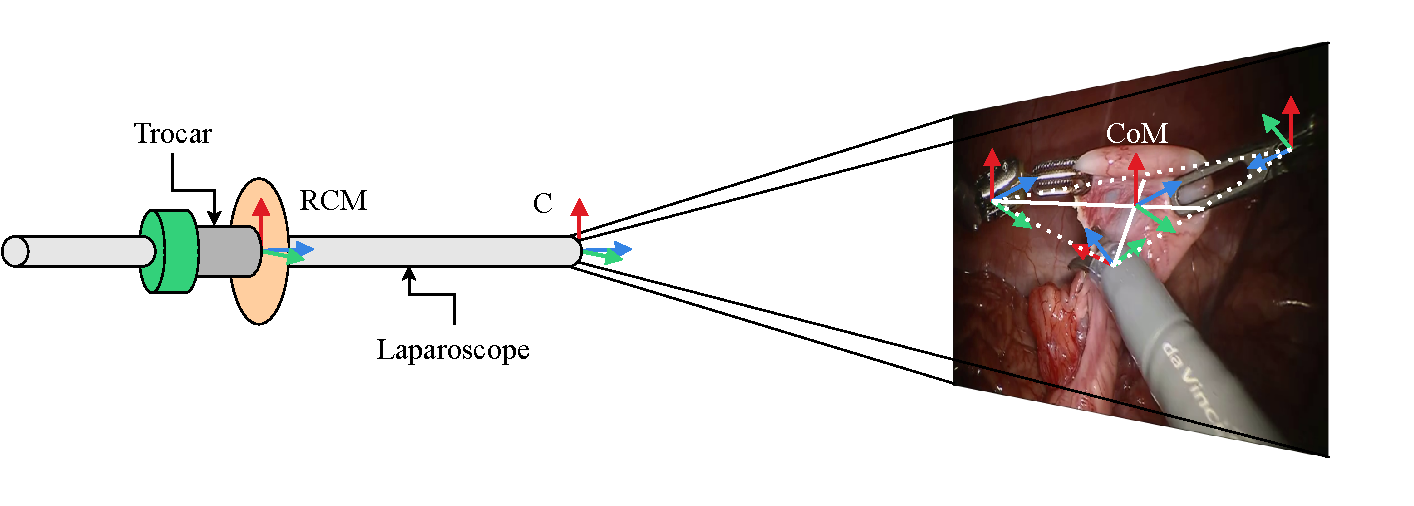
\includegraphics[width=\textwidth]{introduction/fig/rule_based_approaches.pdf}
    \caption{Coordinate frames relevant for laparoscopic camera motion automation. Camera frame C, center of mass frame \gls{com}, and \gls{rcm} at trocar. The camera frame C is commonly obtained via eye-in-hand calibration, \secref{in:sec:eye_in_to_hand_calibration} and \figref{in:fig:eye_in_hand_setup}. For visual servoing, the \gls{com} assumption as view center-point in commonly made. Laparoscopic view shows an image from a da Vinci\textsuperscript{\textregistered} system in the SurgVisDom\cite{zia2021surgical} dataset. Refers to \secref{in:sec:rule_based_approaches}.}
    \label{in:fig:com}
\end{figure}
Laparoscopic camera motion can be automated in a plenitude of ways. A typical laparoscopic setup is shown in \figref{in:fig:com}. Therein, the ultimate goal is to control the pose of the camera frame C under the \gls{rcm} constraint. The camera frame C, as was explained in 
\secref{in:sec:camera_intrinsic_calibration}, and \secref{in:sec:eye_in_to_hand_calibration}, \figref{in:fig:eye_in_hand_setup}, can be obtained through camera intrinsic parameters plus eye-in-hand calibration.

In fully robotic setups, a common approach to automation is to simply use the kinematic data that is available through the joint position encoders~\cite{da2020scan}. The camera then follows some geometric point, like the center of mass between the tools, as shown in \figref{in:fig:com}. Without the kinematic data, these methods are not applicable to hybrid setups, which are of particular interest to this work, as was mentioned in \secref{in:sec:automation} - Robot-free surgeries. They further suffer some other shortfalls, such as the inability to obey by anatomic constraints and reliance on accurate multi-arm calibrations. Other, semi-autonomous techniques, aim to alleviate some of the model uncertainties by assigning the surgeons a greater responsibility to controlling the camera in a collaborative fashion. Gaze or voice control are among them~\cite{taniguchi2010classification}. They, however, lead to eye strain, additional mental workload or communication failures, and do not satisfy the - level five: high autonomy - target that was set in \secref{in:sec:foreword}.

% ji2018learning, su2020multicamera, wagner2021learning

Alongside automation via kinematic data, visual servoing, i.e. control through images, is considered a promising alternative, as it provides intra-operative feedback~\cite{pandya2014review} and is less prone to errors from model mismatch~\cite{azizian2014visual}. It is capable of understanding and interpreting the surgical scene, thus potentially enabling level five autonomy and above, the overarching goal of this work, \secref{in:sec:foreword}. Visual servoing, in itself, is of special interest to this work for one additional reason.
\begin{figure}[htb]
    \centering
    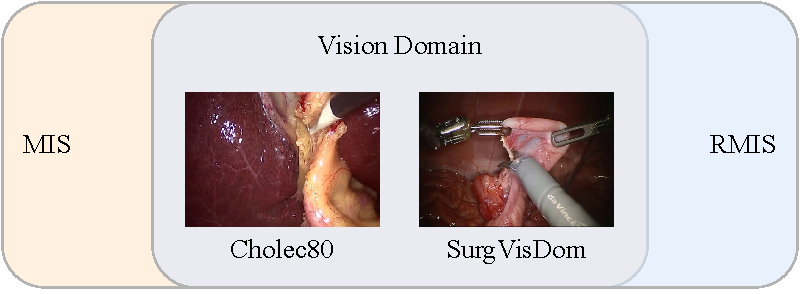
\includegraphics{introduction/fig/shared_domain.pdf}
    \caption{The vision domain is a shared domain between \gls{mis} and \gls{rmis} procedures. Laparoscopic views taken from Cholec80~\cite{twinanda2016endonet}, and SurgVisDom~\cite{zia2021surgical}. Refers to \secref{in:sec:automation_approaches}.}
    \label{in:fig:shared_domain}
\end{figure}
It characterizes \gls{mis} to \gls{rmis} transferability, as was targeted in \secref{in:sec:enhancing_current_systems}. Vision poses a shared domain between \gls{mis} and \gls{rmis}, the vision domain, as shown in \figref{in:fig:shared_domain}. Visual servoing methodologies could thus be transferred from \gls{mis} to \gls{rmis} and vice-versa. In the next section, we will, therefore, review rule-based visual servoing approaches.

\subsection{Rule-based Visual Servoing}
\label{in:sec:rule_based_approaches}
Rule-based visual servoing approaches are a well established research field for laparoscopic camera motion automation. These methods are formulating control through specifying some proxy for autonomy. There exists research on visual servoing with mechanical \gls{rcm} and visual servoing with programmable \gls{rcm}. Although areas aim at controlling the camera frame, refer \figref{in:fig:com}, we will distinguish between them for better clarity and to comply with the targets that were outlined in \secref{in:sec:enhancing_current_systems}. The following two paragraphs will, therefore, review current rule-based approaches with mechanical and programmable \gls{rcm}, respectively, followed by a paragraph that analyzes the shortcomings of these methods.

\paragraph{Visual Servoing with mechanical \gls{rcm}}
Approaches that use a mechanical \gls{rcm} are~\cite{omote1999self}, where a visual servo is implemented to control the center of mass of a colored marker on a forceps in image space. In~\cite{agustinos2014visual, voros2007automatic}, the tool tip position is found in image space via kinematic knowledge over the tool entry points and a visual servo is applied to center the tool tip in image space. Another common scheme is to alter the camera's zoom based on the distance of the surgical tools, which was first presented in~\cite{king2013towards}, where the authors use colored markers to track the surgical instruments.

The authors in~\cite{eslamian2020development, mariani2020experimental, da2020scan}, with related prior works in~\cite{Eslamian2016TowardsTI, eslamian2017autonomous}, compute the center point in between two surgical tools via their respective positions and align the camera's optical axis with the line that spans from \gls{rcm} to the tools' center point, which requires a complicated registration procedure.~\cite{yu2016automatic} also relies on the positions of the surgical tools and adjusts the field of view's width based on the distance of them.~\cite{abdelaal2020orientation} uses a similar approach as~\cite{eslamian2020development}, in that they adjust the camera distance to the surgical scene based on the tool distance, however, they don't align the camera's optical axis with the line that spans from \gls{rcm} to the camera, but rather with the scene's surface normal, which is made possible by their 6 \gls{dof} endoscope. In~\cite{ma2019autonomous}, Ma et al. deploy a visual servo to center a green marker on a tool by incorporating depth information as extracted from camera and tool motion. In~\cite{ma2020visual} they extend this work into a quadratic program in which they minimize joint velocities whilst constraining the camera's distance with respect to the tools and the average tool position in the image plane to be central, where they rely on stereoscopic images to extract depth information.~\cite{gruijthuijsen2021autonomous} propose a framework for semantically rich collaborative control but effectively only track surgical tools.



% Automation in robot-assisted minimally invasive surgery (RMIS) may reduce human error that is linked to fatigue, lack of attention and cognitive overload~\cite{fiorini2022concepts}.
%It could help surgeons operate such systems by reducing the learning curve~\cite{van2018learning}.
%And in an ageing society with shrinking workforce, it could help to retain accessibility to healthcare. It is therefore expected that parts of \gls{rmis} will be ultimately automated~\cite{davenport2019potential,zidane2022robotics}. On the continuous transition towards different levels of autonomy, camera motion automation is likely to happen first~\cite{kitaguchi2022artificial}.



\paragraph{Visual Servoing with programmable \gls{rcm}}
Where a mechanical \gls{rcm} is not available, it can be achieved programmatically. As such,~\cite{aghakhani2013task} design a composite Jacobian method that integrates a \gls{rcm} objective with a task function that defines an error on points in image space. The authors in~\cite{yang2019adaptive} also design a Jacobian gain controller that enforces the tip of a tool to reside within a defined region by computing the winding number of that region around the desired point. They additionally request the endoscope to extend the surgeon's natural line of sight. In~\cite{li2020accelerated}, Li et al. introduce the \gls{rcm} and a visual error via the image Jacobian as constraints to a quadratic problem that aims at satisfying these constraints whilst minimizing the joint velocities.~\cite{sandoval2021towards} propose a torque control framework that includes remote center of motion constraints, tool center point following and nullspace projects for arm-staff collisions.

\paragraph{Flaws of current Visual Servos} It becomes apparent that most of these methods rely on the mere tool distance to infer a control law, whereas only in~\cite{ma2019autonomous, ma2020visual, aghakhani2013task, yang2019adaptive, li2020accelerated} the image points for visual servoing can be chosen arbitrarily. This leaves most of the current methods with some fundamental flaws. First, the assumption that laparoscopic camera motion only originates from tool motion, but not from surrounding tissue or organs. However, clinical evidence suggests camera motion is also caused by the surgeon’s desire to observe tissue~\cite{ellis2016task}. Surgeons might be interested in examining specific anatomy, e.g. for establishing the critical view of safety, refer \secref{in:sec:critical_view_of_safety}. This claim can easily be verified by the interested reader through watching videos of laparoscopic interventions. Second, all of these methods are of reactive nature and none of them anticipates future potential views. Only in~\cite{weede2011intelligent} and~\cite{ji2018learning}, the authors consider predictive models based on expert demonstrations. In~\cite{weede2011intelligent}, Weede et al. cluster gripper positions in observed interventions and compute transition probabilities from cluster to cluster by modelling the system as a Markov chain. They predict the probability of future tool positions and enforce the camera's optical axis to point to the future probability weighted sum of the tools' positions, which relies on kinematic information. Ji et al. propose in~\cite{ji2018learning} to rank image features in object bounding boxes according to expert demonstrations with a linear regression, however, they don't consider an \gls{rcm} or any constraints in motion that arise from it and only regress their model on a synthetic environment. It remains questionable whether this method could be transitioned to a real setup.

\subsection{Auxiliary Vision Tasks}
\label{in:sec:auxiliary_tasks}
% slowly paving their way into...
% tool segmentation , surgical phase recognition, pose estimation, depth estimation
\begin{figure}[tb]
    \centering
    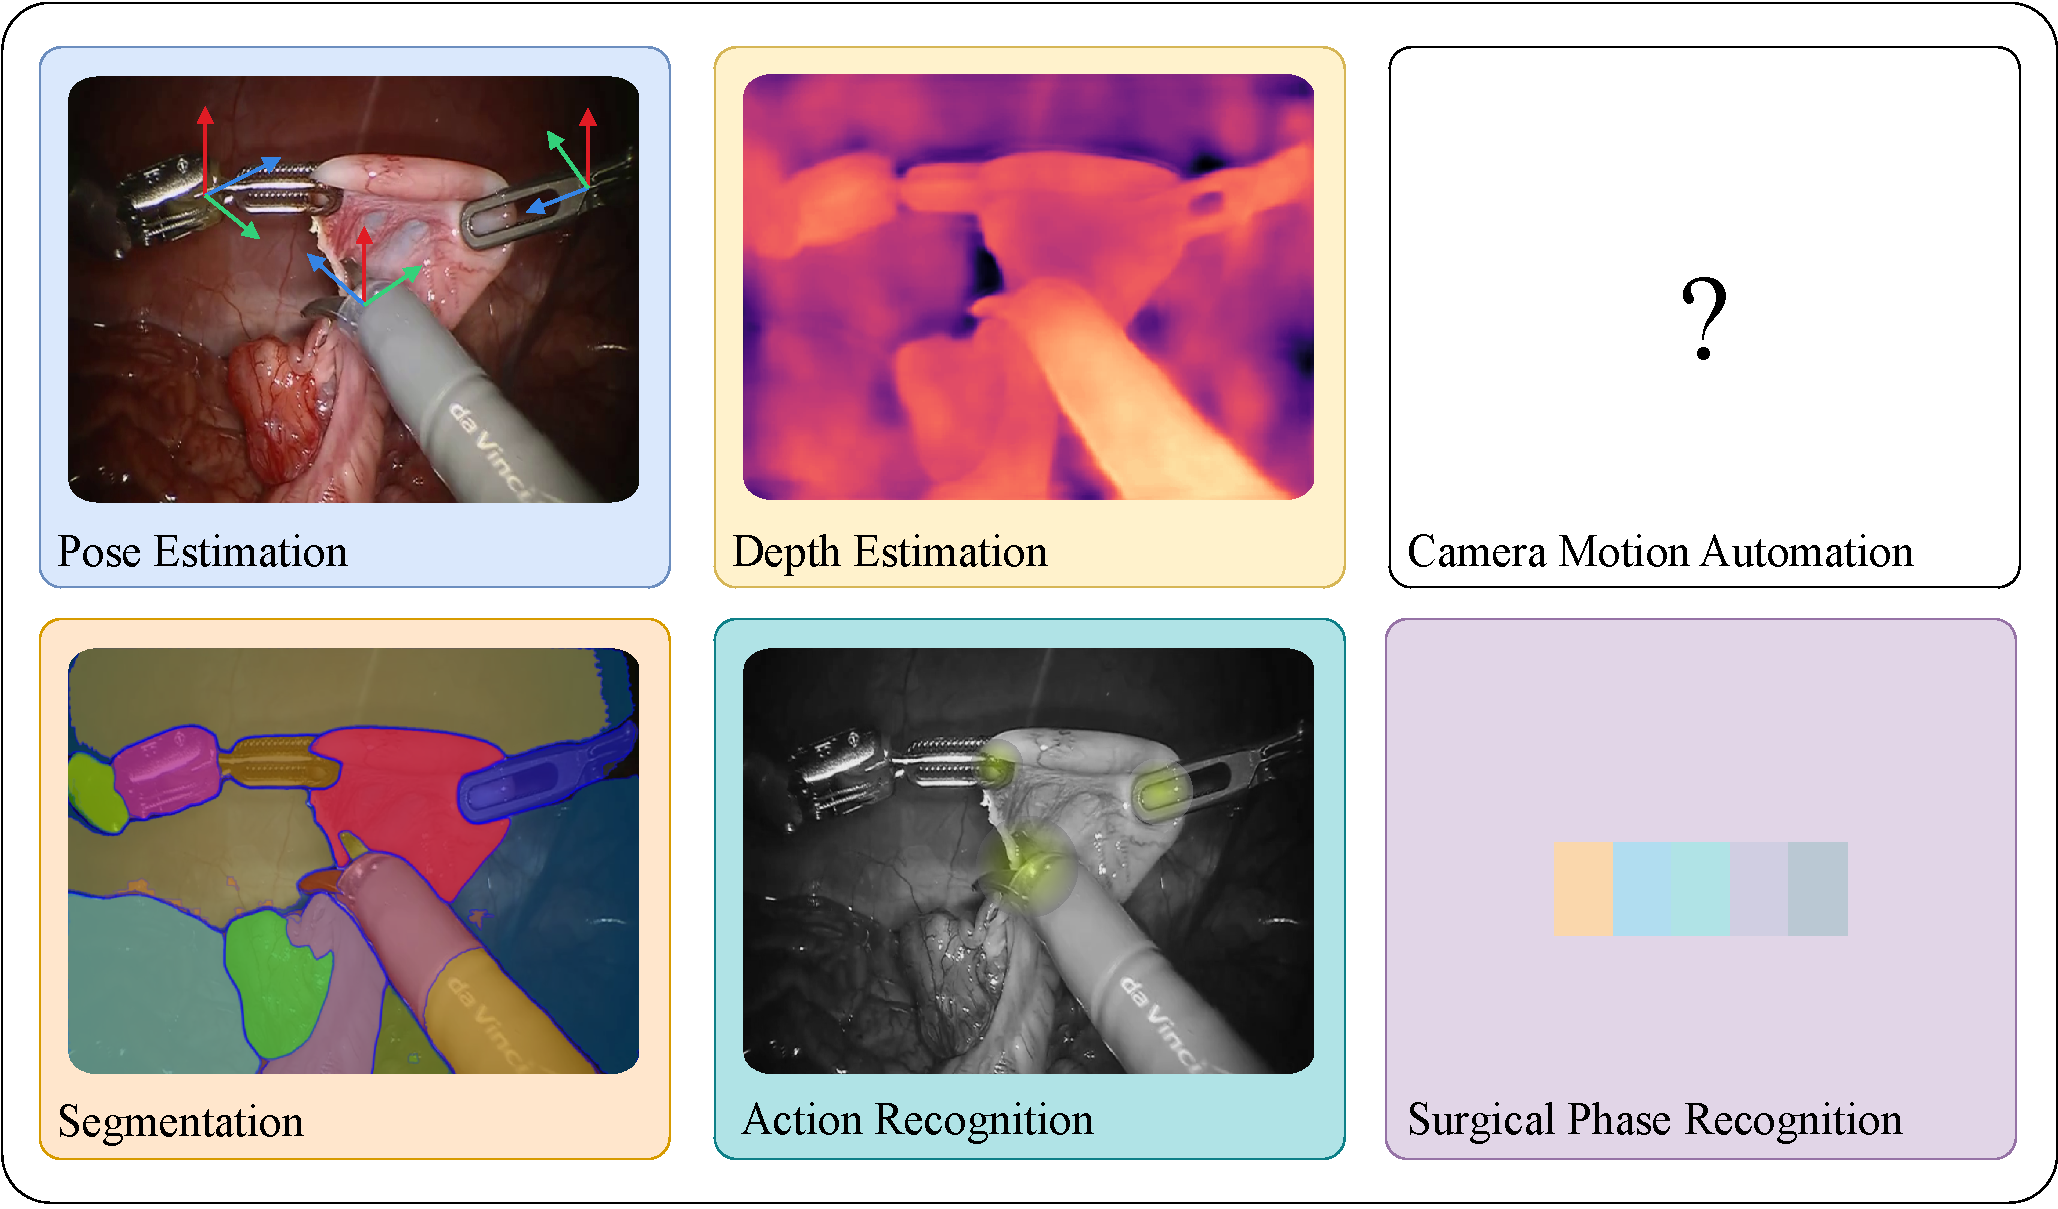
\includegraphics[width=\textwidth]{introduction/fig/auxiliary_tasks.pdf}
    \caption{Auxiliary tasks that could be used for laparoscopic camera automation but that are not used in practise. None of the data-driven methods directly attempts laparoscopic camera motion automation in realistic scenarios. The surgical phases refer e.g. back to \secref{in:sec:cholecystectomy_procedure}. Laparoscopic view shows an image from a da Vinci\textsuperscript{\textregistered} system in the SurgVisDom~\cite{zia2021surgical} dataset. Monocular depth estimated using~\cite{oquab2023dinov2}, segmentations generated through~\cite{segment_anything}. Refers to \secref{in:sec:auxiliary_tasks}.}
    \label{in:fig:auxiliary_tasks}
\end{figure}
Apparently, current visual servos oversimplify the automation task greatly. Only~\cite{gruijthuijsen2021autonomous} incorporate neural networks for autonomous instrument tracking. What is generally lacking is an understanding for the surgical scene that could help overcome the simplifications that are currently made for visual servoing. Indeed, there exists plenty of research on solving auxiliary vision tasks through data-driven methods, see \figref{in:fig:auxiliary_tasks}. Some of which, will be highlighted below. 

\paragraph{Automation-related Tasks} Based on progress in segmentation tasks, using deep learning, but also with the prospect of identifying tool tips for automating procedures, a vast body of literature on surgical tool segmentation evolved, including~\cite{allan20192017, pakhomov2019deep}, and~\cite{garcia2016real, garcia2017toolnet, shvets2018automatic, islam2019real, jin2018tool, sarikaya2017detection, da2019self, attia2017surgical, laina2017concurrent, garcia2021image}. Some of these segmentation works help improve surgical tool pose estimation, as was shown in~\cite{kurmann2017simultaneous, li2020super, hasan2021detection}, as does monocular depth estimation~\cite{li2020unsupervised,huang2021self,xu2022self, shao2022self,li2023multi,lou2024wssfmlearner,budd2024transferring} and~\cite{li2022geometric,bardozzo2022stasis,huang2022simultaneous,huang2022self}. Whilst these works could be fused with any of the visual servos from above, it wouldn't resolve the general assumption that camera motion only results from tool motion. Besides tool segmentation, research exists for surgical phase detection~\cite{stauder2014random, lalys2014surgical, jin2016endorcn, dergachyova2016automatic,twinanda2016endonet,malpani2016system, jin2017sv, ross2018exploiting, yengera2018less, funke2018temporal, yu2018learning} as well as~\cite{bodenstedt2019active, padoy2019machine, czempiel2020tecno, jin2020multi, kitaguchi2020real}. These could condition visual servos on the current phase of the surgery. Other self-supervised approaches, which could be integrated similarly, aim to estimate the remaining time of a surgical procedure~\cite{twinanda2018rsdnet, bodenstedt2019prediction, rivoir2019unsupervised} or perform action recognition~\cite{nwoye2021deep}.

\paragraph{The Automation Task} Automation-related tasks, as introduced in the previous paragraph, are often treated as prerequisite for autonomy, but could at present only contribute as input to a smarter visual servoing scheme. Given the success of data-driven methods for these auxiliary tasks, it might be reasonable to utilize them for laparoscopic camera motion automation as well. But instead of taking any of the auxiliary tasks as priors, one might consider learning automation directly, too. This is because, firstly, in deep learning, end-to-end approaches have proven to outperform methods that rely on hand-crafted inputs that may seem humanly logical, and, secondly, it is the simplest approach. So instead of extracting redundant information, such as tool tips, surgery phases, depth, or poses first, we suggest that it might make sense to apply data-driven methods to automating laparoscopic camera motion immediately. This sentiment is supported by related fields, where learning policies on vast amounts of data has demonstrated great success with the emergence of complex behaviors, far more complex than the tool following proxy. Interestingly, data-driven laparoscopic camera motion automation is an underexplored field. In spite of the underexploration of data-driven methods for laparosopic camera motion automation, we turn to a broader body of literature, and introduce several learning-based methods in the next sections, namely reinforcement learning in \secref{in:sec:reinforcement_learning}, and imitation learning in \secref{in:sec:imitation_learning}.

% Put differently, why would one have to segment surgical tools first to extract a control policy, instead of immediately inferring the control policy? 

% From an algorithmic perspective, both approaches should be equally demanding tasks, while the latter doesn't constrain the method in its solution. 

% but also apparant that other methods are necessary to .. complex behavior

% Let alone this realization out-rules all visual servoing approaches that rely on tools only as potential candidates for fully automating camera movement in laparoscopic surgery. 

% Extracting camera motion from images is a well studied problem, but not so much in the surgical context, where an extremely dynamic and deformable environment with little texture hardens the task. 

% Therefore, simplifying the problem is crucial. In its simplest form, one can model a surgical scene as a plane, camera motion can hence be described as a homography and recent advances in deep homography estimation have successfully extracted homographies from images with little texture~\cite{detone2016deep, erlik2017homography, nguyen2018unsupervised}. These findings were further applied in the surgical realm by Gomes et al. in~\cite{gomes2019unsupervised} and by Bano et al. in~\cite{bano2020deep}. Bano et al. further refined their findings in~\cite{bano2020vessel} by segmenting veins for the registration process. Yet, none of the above methods takes dynamic scenes into consideration. Most recent literature on deep homography estimation demonstrated how deep homography estimation can be applied to dynamic scenery~\cite{le2020deep, zhang2019content}.


\subsection{Reinforcement Learning}
\label{in:sec:reinforcement_learning}
\begin{figure}[htb]
    \centering
    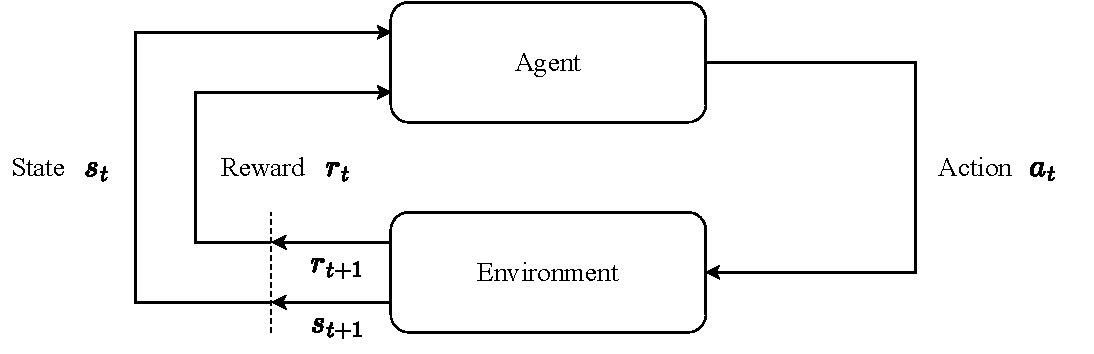
\includegraphics[width=\textwidth]{introduction/fig/reinforcement_learning.pdf}
    \caption{A procedural diagram of reinforcement learning. Given the environment state $s_t$, an agent performs an action $a_t$ and observes the resulting state $s_{t+1}$ and reward $r_{t+1}$. Refers to \secref{in:sec:reinforcement_learning}.}
    \label{in:fig:reinforcement_learning}
\end{figure}
\gls{rl} is conceptually simple and hence so appealing. It, at least in parts, seems to mimic some of the human characteristics for acquiring new skills. In a \gls{rl} scenario, see \figref{in:fig:reinforcement_learning}, an agent interacts with an environment. The agent observes state $s_t$ and performs an action based on it. The agent will then observe the changed state $s_{t+1}$ and receive a reward $r_{t+1}$. Through trial and error, the agent will try to maximize the reward. \gls{rl} is sample inefficient and requires a large amount of trials until the agent learns to solve a task successfully. \gls{rl} is in fact so sample inefficient, that it is often applied to simulation, where physical systems can be mimicked far beyond realtime. If a system can be simulated well, then \gls{rl} can find impressively complex behaviors in vast state spaces that could not be explored through classical search algorithms. This is why there exists impressive research in \gls{rl}, where it was e.g. shown that agents can learn to play Atari games just through observing images~\cite{mnih2013playing}. This success lead to systems that are capable of beating humans in the game of Go~\cite{silver2016mastering}, which was later improved to learn entirely through self-play~\cite{silver2017mastering}. For reference, there exist many more possible states in Go than there are atoms in the known universe. These two examples stem from easily simulatable environments (Go and Atari games) without physics. But even in physically more challenging scenarios, it was shown that humanoid walking can be solved through \gls{rl}~\cite{schulman2017proximal}. The transferability from simulation to the real systems, however, was left unsolved. The most recent advancements succeeded in transferring highly complex policies from simulation to real robots, like standing up~\cite{rudin2022learning} or parkour~\cite{hoeller2023anymal} on the ANYmal quadruped, and playing football on a simplified humanoid robot~\cite{liu2022motor}. The state of simulation in surgery will be summarized in the next paragraph.

\paragraph{Laparoscopic Camera Motion Automation}
\begin{figure}[tb]
    \centering
    \begin{subfigure}[b]{0.49\textwidth}
        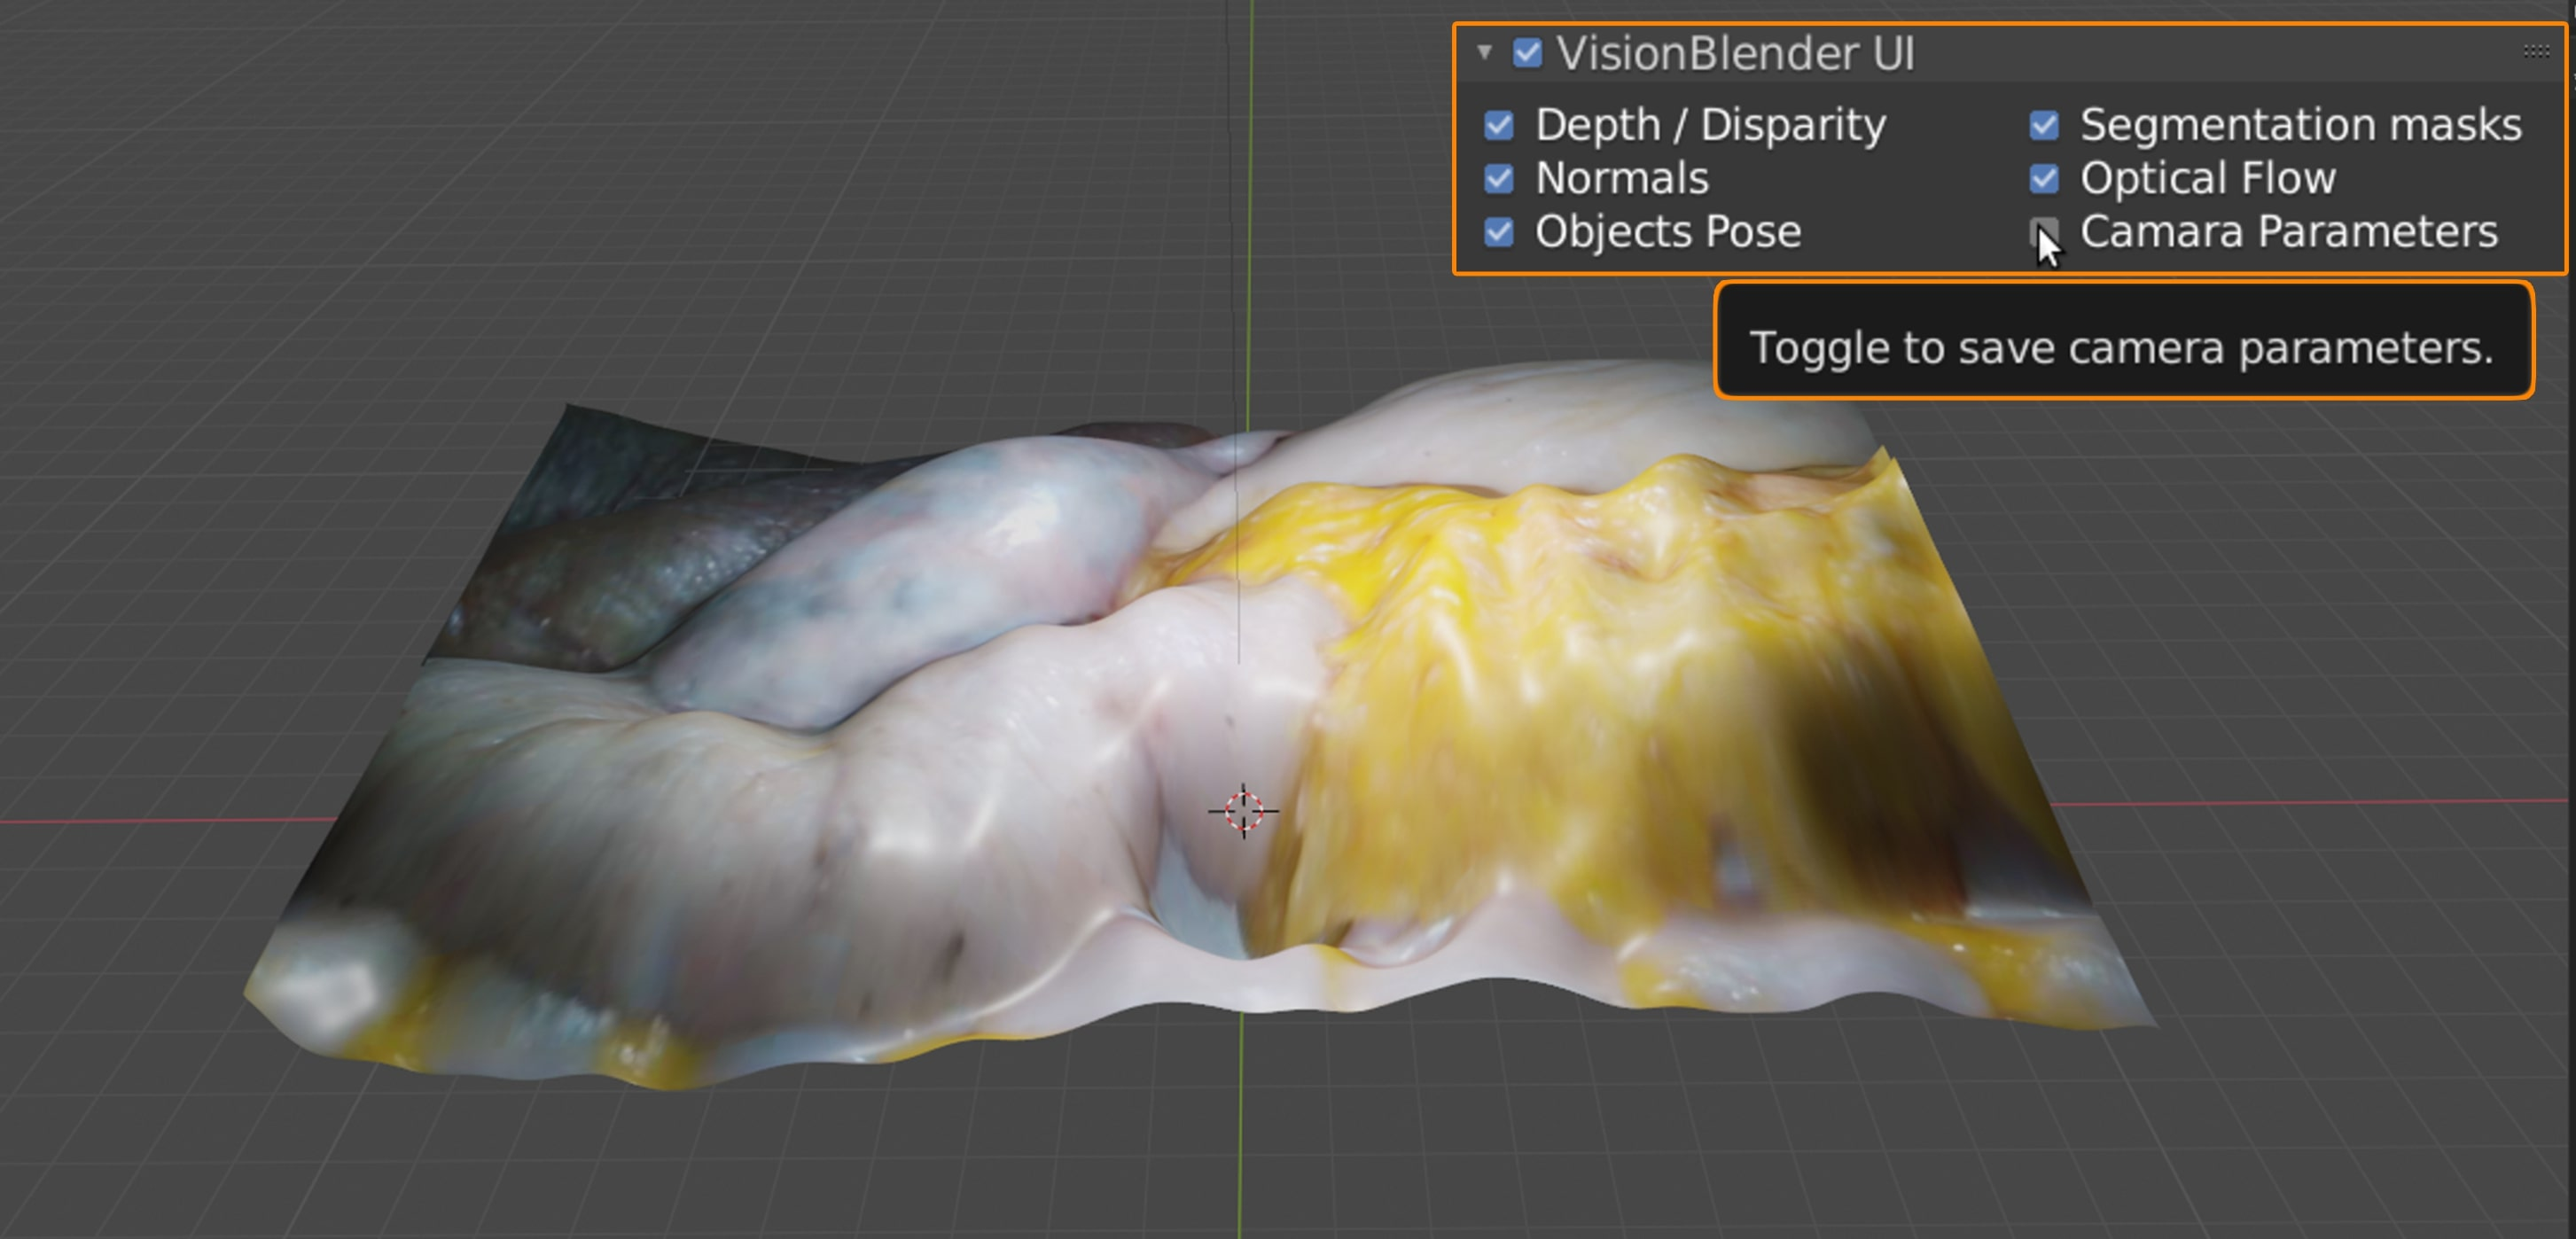
\includegraphics[width=\textwidth]{introduction/img/vision_blender_view.jpg}
        \caption{Static surgical 3D scene.}
    \end{subfigure}
    \begin{subfigure}[b]{0.49\textwidth}
        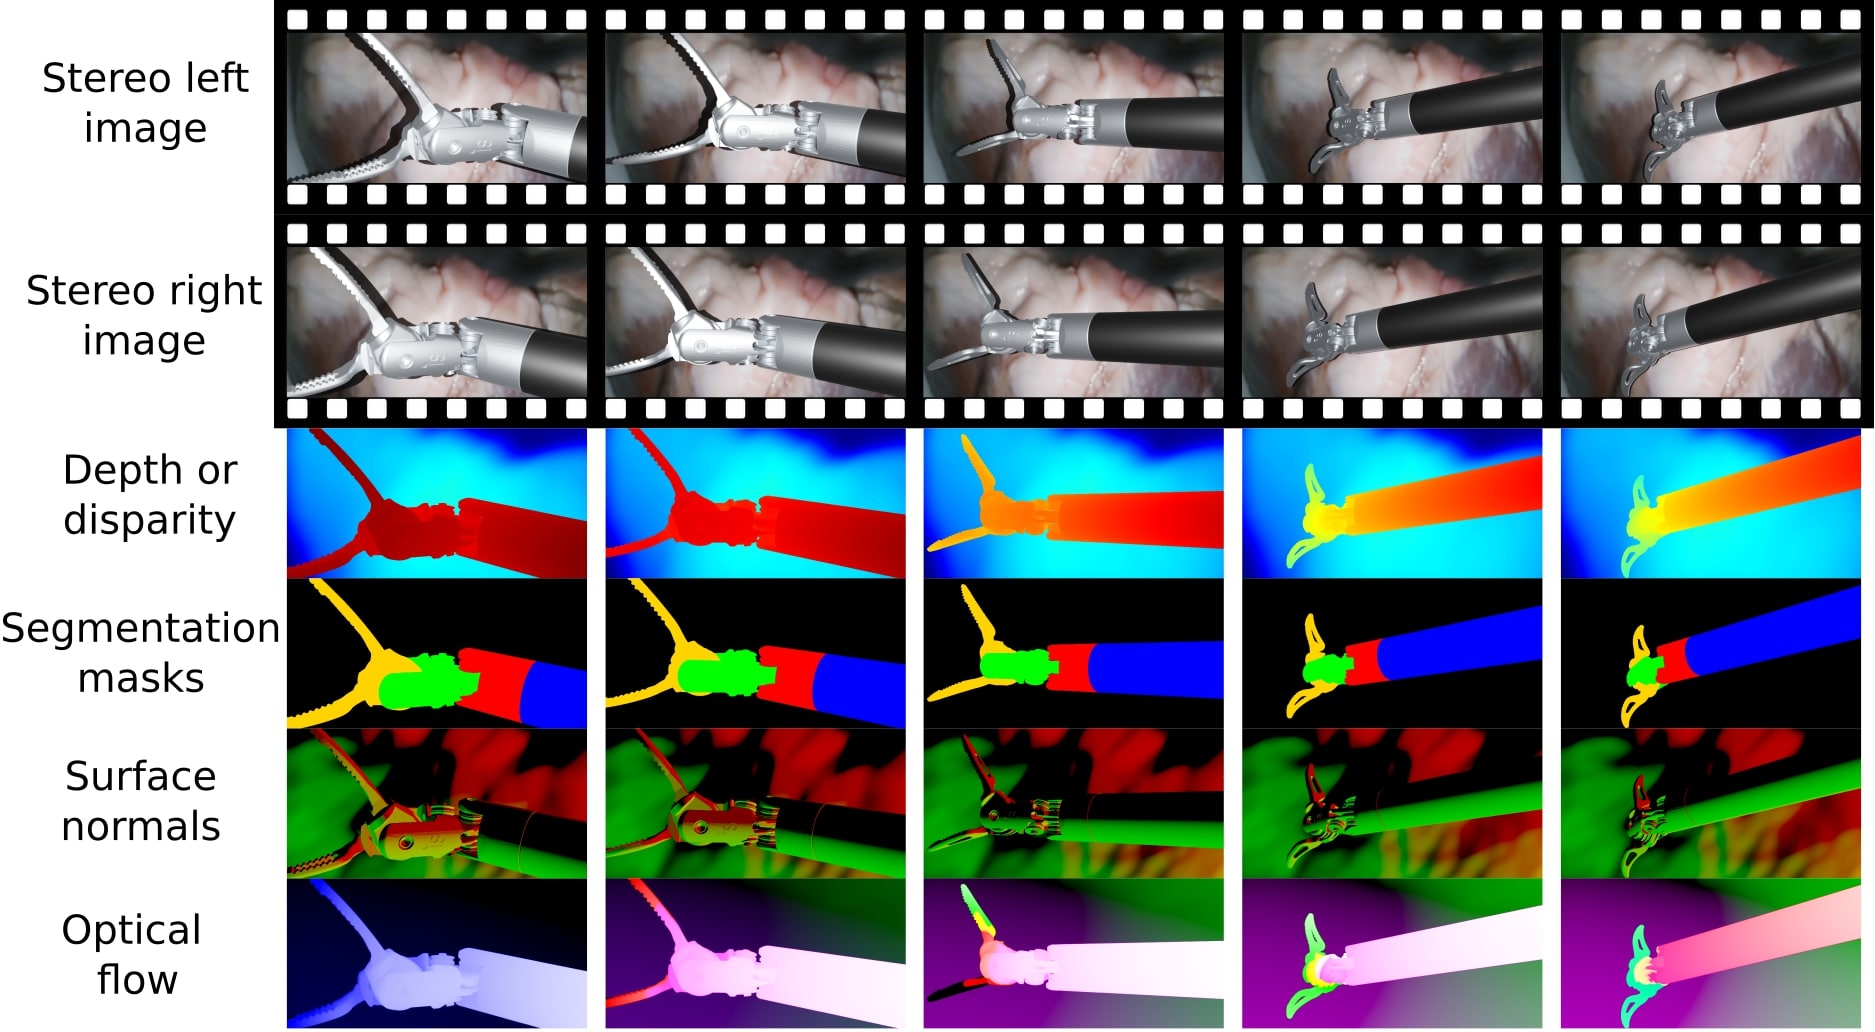
\includegraphics[width=\textwidth]{introduction/img/vision_blender_masks.jpg}
        \caption{Generated masks.}
    \end{subfigure}
    \caption{Blender plugin, named Vision Blender, for rendering realistic surgical scenes. Images with courtesy of~\cite{cartucho2021visionblender}. Refers to \secref{in:sec:reinforcement_learning}.}
    \label{in:fig:vision_blender}
\end{figure}
The hurdles for \gls{rl} in laparoscopic camera motion automation are obvious. The sample inefficiency and potential harm to patients currenty restrict \gls{rl} approaches to simulation~\cite{su2021multicamera,agrawal2018automating}. Significant steps are being made to improve simulations, like~\cite{scheikl2023lapgym} using e.g. SOFA~\cite{allard2007sofa}, but a domain gap remains. Research that attempts to bridge the domain gap to make \gls{rl} algorithms deployable in real setups exists,~\cite{cartucho2021visionblender} e.g. provide a Blender plugin for realistic view generation, see \figref{in:fig:vision_blender}, and~\cite{marzullo2021towards} propose image domain transfer, but only static scenes are considered for now. Clinical translation using \gls{rl} has yet to be achieved.

We conclude that \gls{rl} does not comply with the objective of this thesis, that is near term automation that benefits the patient, refer \secref{in:sec:foreword}. This is because simulations have not yet reached the realism that is required for narrowing the domain gap to surgery. Therefore, the next \secref{in:sec:imitation_learning}, will investigate other data-driven methods instead.

\subsection{Imitation Learning}
\label{in:sec:imitation_learning}
The goal of \gls{il} is to copy the behavior of an expert demonstrator. Hence, \gls{il} aims to extract an expert policy $\pi_\text{E}: s_t \rightarrow a_t$ that maps a state $s_t$ to an action $a_t$, where the actions and states are drawn from a trajectory $\tau_i = \{s_t,a_t...,x_{t+T+1},a_{t+T+1}\}$, sampled from expert demonstrations $\tau_i \in D$. The underlying state $s_t$ might not always be fully observable, in which case one observes $\hat{s}_t = f(s_t)$, where $f$ is the unknown mapping of the underlying state $s_t$ to the observed state $\hat{s}_t$. \gls{il} without access to the underlying state is often referred to as \gls{ifo}~\cite{liu2018imitation}. Also, the embodiment of demonstrator and learner might not always be the same, e.g. if the demonstrator is a human and the learner is a robot, which is called a domain shift. \gls{il} is usually achieved via either of two dominant approaches~\cite{osa2018algorithmic}: \gls{bc}~\cite{pomerleau1991efficient} and \gls{irl}~\cite{ng2000algorithms}. \gls{bc} regresses the expert policy $\pi_\text{E}$ from sampled trajectories $\tau_t$ in a supervised fashion. \gls{irl} aims to recover the expert's hidden reward $r_t$ to later optimize a policy to also achieve the recovered reward. Neural networks have become the dominant approach for estimating the policy $\pi$, henceforth, the following sections will focus on them.

\subsubsection{Behavioral Cloning}
In a common \gls{bc} setup that satisfies the Markov property one takes a current state and tries to predict future actions conditioned only on the current state. One can also condition actions on a set of past states~\cite{xu2017end} but this is rather uncommon. In~\cite{torabi2018behavioral}, Torabi et al. try to perform \gls{ifo} by randomly exploring the action-state space. They learn a mapping from observations to actions and perform \gls{bc} on newly obtained observations via this mapping. A general issue in \gls{bc} is covariate shift, that is the inability to generalize on a small dataset. In~\cite{ho2016generative}, Ho et al. address this issue by introducing generative adversarial learning which implicitly regularizes the policy to a bigger action-state space.~\cite{torabi2018generative} extends~\cite{ho2016generative} by working without immediate access to actions but from observation only. Although generative adversarial imitation learning helps to generalize, a lot of the existing literature focusses on learning an underlying forward dynamics model to infer any policy once the forward dynamics model is known. As such, the authors in~\cite{finn2016unsupervised, finn2017deep, nair2017combining} learn to predict future observations from actions via a dataset of randomly explored action-state space trajectories. They use this state transition model to infer actions that lead to desired states, which requires the user to define a desired state. Other attempts to learn arbitrary behaviors are one-shot and zero-shot imitation learning approaches. In one-shot~\cite{finn2017one}, Finn et al. use \gls{maml} to learn how to learn new tasks quickly. Once the network parameters are initialized via meta-learning, a few gradient steps from a demonstration allow to imitate that demonstration. In~\cite{yu2018one}, Yu et al. extend this work across domain gaps, that is a robotic learner imitates a human demonstrator from a single demonstration only. Pathak et al. then introduce zero-shot learning in~\cite{pathak2018zero}, which introduces a goal conditioned policy, that allows to immediately execute a policy from intermediate pre-defined goal states. In~\cite{hausman2017multi}, Hausman et al. extend the work in~\cite{ho2016generative} by conditioning the policy on the intention, which similarly to zero-shot imitation learning, allows to reach intermediate goals. The idea of learning a forward dynamics model is then extended into a compressed feature space by Srinivas et al. in Universal Planning Networks~\cite{srinivas2018universal}. Their work conditions latent-space dynamics on actions from demonstrations and they define an optimization framework that finds actions conditioned on a goal state. Most recent approaches, such as~\cite{lynch2020learning}, learn a latent state representation that categorically clusters different policies as to create interpretable behaviors.


\subsubsection{Inverse Reinforcement Learning}
In \gls{irl} the aim is to extract a reward function from a set of expert demonstrations $D$. In practise this can be achieved by embedding observations $\hat{s}_t$ into a meaningful feature space and by enforcing that a newly obtained policy $\pi$ and an expert policy $\pi_\text{E}$ follow similar trajectory embeddings.

Different methods for embedding exist. A triplet loss can be formulated to pull similar images closer to each other while repelling them from different ones. In~\cite{wang2014learning, schroff2015facenet}, the authors achieve a triplet loss via a simple distance metric while Wang et al. formulate it as the angle between features~\cite{wang2015unsupervised}. Another option is to use prediction as a proxy for meaningful embeddings~\cite{vondrick2016anticipating, sermanet2016unsupervised, srivastava2015unsupervised, mathieu2015deep}, self-supervised clustering~\cite{caron2018deep}, or, most recently, contrastive learning methods~\cite{khosla2020supervised}, which similarly to~\cite{wang2015unsupervised} aim to align features of samples with similar properties.

Sermanet et al. in~\cite{sermanet2018time} used for example a triplet loss on multi-view videos to learn a view-point invariant embedding that can be used to have a learner learn an expert demonstration. Aytar et al. in~\cite{aytar2018playing} had an agent learn to reach checkpoints by sampling checkpoints from demonstrations on YouTube and by defining a reward on the alignment between the current state and the desired checkpoint. In few-shot, Xie et al.~\cite{xie2018few} learn initial parameters for a network via \gls{maml}, a form of meta-learning, to infer goals in demonstrations from a single gradient-step. They then perform \gls{rl} to replicate a policy that yields these goals. The idea of Universal Planning Networks by Srinivas et al. in~\cite{srinivas2018universal} is further extended by Yu et al. in~\cite{yu2019unsupervised}, which learns a goal metric for \gls{rl} in an unsupervised manner.

\section[Imitation Learning for Robotic Laparoscopy]{Imitation Learning for Laparoscopic Camera Motion Automation}
\label{in:sec:imitation_learning_for_camera_motion_automation}
In the previous sections, several considerations that are relevant to achieving laparoscopic camera motion automation, including economical, clinical, and technical aspects, were introduced. Plenty arguments went into the decision making and some of which may have already been forgotten. Therefore, in this section, we will revisit the key-concepts in \secref{in:sec:revisiting_key_concepts}. Next, and given these critical considerations, we will hypothesize a method for laparoscopic camera motion automation in \secref{in:sec:hypothesizing}, followed by several sections on realizing the hypothesized approach.

\subsection{Revisiting Key Concepts}
\label{in:sec:revisiting_key_concepts}
\paragraph{The Case for Camera Motion Automation} In the Foreword, \secref{in:sec:foreword}, it was argued that the progressive nature of surgery will ultimately alleviate clinical staff of unfulfilling tasks through achieving level five autonomy, likely first for laparoscopic camera motion. We took the clinicians' perspective in the cholecystectomy procedure, the most common laparoscopic procedure, to investigate automation claims further. We found that the camera holder assistant, see \figref{in:fig:room_setup}, performs a relatively simple and unfulfilling task. This stays in contrast with the importance of the camera holder's role of establishing and maintaining a good view for highlighting critical anatomies to surgeons, \secref{in:sec:cholecystectomy_procedure}. We then analyzed the rise of \gls{rmis} in \secref{in:sec:the_rise_of_robot_assisted_laparoscopy}, and found first indicators that, in \gls{rmis}, the camera is moved more frequently when compared to \gls{mis}, suggesting that even more camera motion might be desirable. This stays is in line with the initial rise of \gls{rmis}. We thus concluded that camera motion automation might be beneficial for the surgeon, the patient, and the clinical staff in \secref{in:sec:enhancing_current_systems}, \figref{in:fig:advancing_robotic_laparoscopy}.

\paragraph{High-level Aspects of Camera Motion Automation}
\begin{figure}[htb]
	\centering
	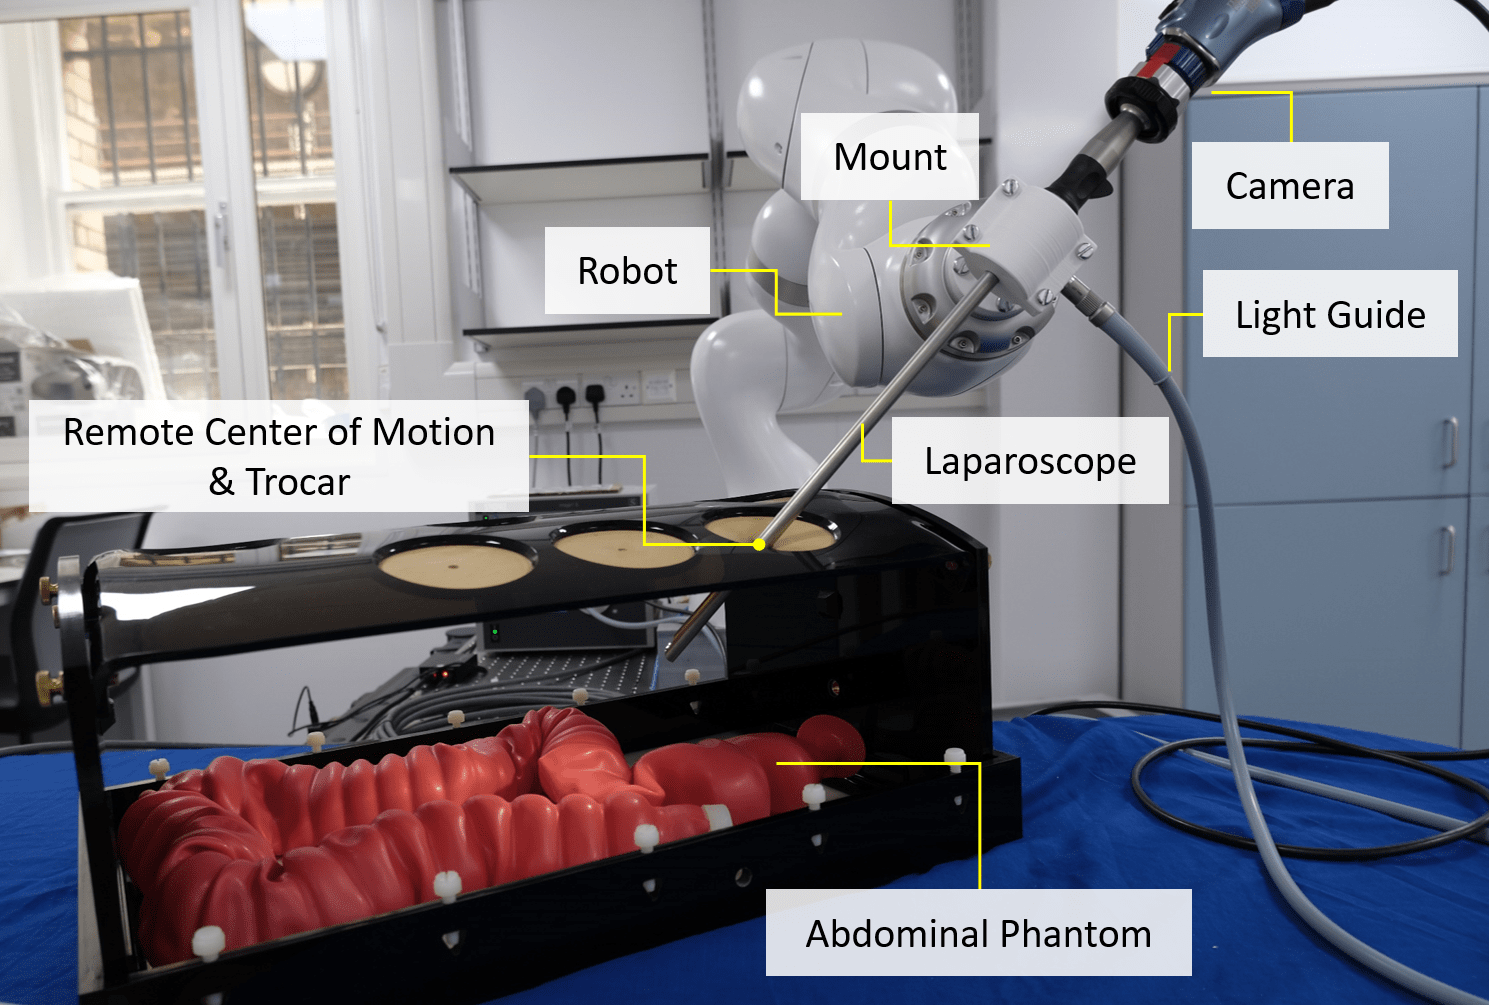
\includegraphics[width=\textwidth]{chapter_2/img/labeled_setup_compressed.png}
	\caption{Robotic setup. A Storz Endocameleon Hopkins Telescope, which provides a light source port and a camera attachment point, is mounted to a KUKA \gls{lbr} Med 7 R800 robot via a 3D printed clamp. The robotic system undergoes image-based control to reach desired views of the surgical scene and simultaneously pivots around a programmable \gls{rcm}.}
	\label{in:fig:experimental_setup}
\end{figure}
We took economical considerations into account for propagating the clinically beneficial automation changes to the patients with minimal impact on cost. This resulted in the goal of delivering the automation endeavor through a system with programmable \gls{rcm} to surgeries that are currently robot-free, \secref{in:sec:automation}. We thus propose a system design that will serve as foundation to this thesis, see \figref{in:fig:experimental_setup}.

Following the clinical prospects of automation and the economically guided form-factor, we analyzed technical factors. We explained calibration prerequisites, \figref{in:fig:eye_in_hand_setup}, \figref{in:fig:com}, and derived novel means of registration for an improved clinical workflow in \secref{in:sec:unified_calibration}, which finally lead to automation itself. We discussed several automation approaches in \secref{in:sec:automation_approaches}, and concluded that learning complex policies, beyond tool following, would require data-driven methods. Crucially, among other reasons, we chose vision as a candidate domain, and thus visual servoing as a candidate for automation, since vision was identified as a shared domain between \gls{rmis} and \gls{mis}, \figref{in:fig:shared_domain}. We found, however, that vision is currently only used for solving auxiliary tasks, \figref{in:fig:auxiliary_tasks}. We evaluated the state of \gls{rl} in \secref{in:sec:reinforcement_learning}, and concluded that it does not align with our goals of near term level five autonomy, and were thus left with imitation learning approaches in \secref{in:sec:imitation_learning}. With the robot-free surgery target in mind, and the suggested imitation learning as substrate for automation, we impose embodiment-invariance onto the solution. That is, the expert demonstrator can be human, and the executing agent is a robot. Precisely speaking, we are, therefore, trying to solve \gls{ifo}, with only access to the partially observed environment state $\hat{s}_t$, see \figref{in:fig:hypothesized_pipeline}. The next sections will go into detail on how this could be achieved concretely.

\subsection{Hypothesizing Embodiment-invariant Laparoscopic Camera Motion Automation}
\label{in:sec:hypothesizing}
\begin{figure}[tb]
    \centering
    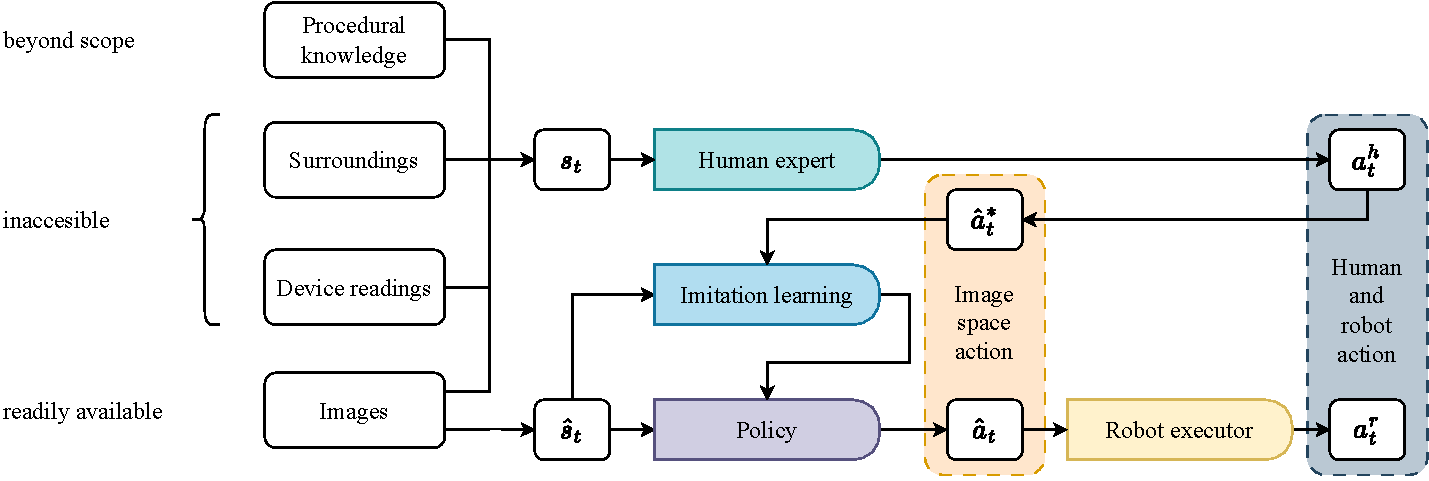
\includegraphics[width=\textwidth]{introduction/fig/camera_motion_action.pdf}
    \caption{The hypothesized approach for laparoscopic camera motion imitation learning. Actions are learned in the shared vision domain and executed via different embodiments, the human or the robot. The human expert has access to the full environment state $s_t$ and performs an action $a^h_t$. This action $a^h_t$, leads to an action in image space $\hat{a}^*_t$, the desired action. We suggest extracting action $\hat{a}^*_t$ from image space for imitation learning purposes. Refers to \secref{in:sec:hypothesizing}.}
    \label{in:fig:hypothesized_pipeline}
\end{figure}
Having outlined the scope for laparoscopic camera motion automation - embodiment-invariant \gls{ifo} - further referred to simply as imitation learning, this section will now hypothesize concrete means of achieving it. It will dissect the thought process for framing the path towards autonomy in this thesis rigorously.

\gls{il} requires large amounts of data for learning the tail-end, i.e. rare cases. Therefore, we will initially search for available data in \secref{in:sec:search_for_available_data}. Given the data, a mixture of supervised and self-supervised methods for learning to predict camera motion, and predicting can be considered imitating, will be suggested in \secref{in:sec:supervised_self_supervised}. Next, a camera motion formulation for the suggested supervised and self-supervised frameworks will be proposed in \secref{in:sec:homography_based_camera_motion_formulation}, keeping the constraint of embodiment-invariance in mind. Finally, \secref{in:sec:robotic_laparoscope_control} will explain classical and clinically applicable methods for controlling a robotic laparoscope under the camera motion prediction.  An overview of the proposed approach is already shown in \figref{in:fig:hypothesized_pipeline}.

\subsubsection{Search for available Data}
\label{in:sec:search_for_available_data}
\begin{table}[htb]
\centering
\caption{Exhaustive overview of publicly available \gls{mis} and \gls{rmis} datasets. All datasets were acquired and analyzed for task-appropriate metrics. Datasets that were not available, or are unreasonable for evaluation, are marked with N/A, where datasets were not available or unreasonable to analyze.}
\label{in:tab:datasets}
\begin{adjustbox}{angle=90, max height=0.85\textheight}
    \begin{tabular}{|c|c|c|r|c|c|c|c|}
        \hline
        \multirow{2}{*}{Collection} & \multicolumn{7}{c|}{Specifications} \\
        \cline{2-8}
        & Name & Year & Length / \# & Frame Rate / Hz & Resolution / pixels & Camera Motion & Note \\
        \hline
        \multirow{8}{*}{\href{https://endovis.grand-challenge.org/}{\shortstack{Endoscopic\\Vision\\Challenge}}} &\href{https://www.synapse.org/#!Synapse:syn21776936/wiki/601700}{MISAW}~\cite{mitsuishi2013master}&2020&$128102$&$30$&$460\times 540$&no&synthetic \\
        \cline{2-8}
        &\href{https://surgvisdom.grand-challenge.org/}{SurgVisDom}~\cite{zia2021surgical}&2020&$185620$&$20$&$540\times960$&occasional&da Vinci\textsuperscript{\textregistered} \\
        \cline{2-8}
        &\href{https://robustmis2019.grand-challenge.org/}{ROBUST-\gls{mis}}~\cite{maier2020heidelberg}\cite{ross2020robust}&2019&$7546968$&$25$&$540\times 960$&yes&laparoscopic \\
        \cline{2-8}
        &\href{https://endovissub2019-scared.grand-challenge.org/}{SCARED}&2019&$16818$&$25$&$1024 \times 1280$&yes& exoscopic \\
        \cline{2-8}
        &\href{https://endovissub-workflowandskill.grand-challenge.org/}{SWASA}&2019&N/A&N/A&N/A&yes& laparoscopic\\
        \cline{2-8}
        &\href{https://endovissub2017-workflow.grand-challenge.org/}{SWASA}&2018&N/A&N/A&N/A&yes& laparoscopic\\
        \cline{2-8}
        &\href{https://endovissub2018-roboticscenesegmentation.grand-challenge.org/home/}{RSS}~\cite{allan20202018}&2018&$2235$&$2$&$1024\times 1280$&occasional& da Vinci\textsuperscript{\textregistered}\\
        \cline{2-8}
        &\href{https://endovissub2017-roboticinstrumentsegmentation.grand-challenge.org/}{RIS}~\cite{allan20192017}&2017&$3225$&$2$&$1024\times 1280$&occasional& da Vinci\textsuperscript{\textregistered} \\
        \cline{2-8}
        &\href{https://endovissub2017-kidneyboundarydetection.grand-challenge.org/}{KBD}&2017&$3000$&$2$&$1024\times 1280$&occasional & da Vinci\textsuperscript{\textregistered}\\
        \cline{2-8}
        &\href{https://endovissub-instrument.grand-challenge.org/}{ISAT}&2015&$16243$&$25$&$480\times 640/576\times 720$& yes & laparoscopic \\
        \hline
        \multirow{3}{*}{\href{http://hamlyn.doc.ic.ac.uk/vision/}{\shortstack{Hamlyn\\Center\\Datasets}}} &\href{http://hamlyn.doc.ic.ac.uk/vision/data/daVinci.zip}{Siamese}~\cite{ye2017self}&2017&$34240$&$30$&$192\times 384$& occasional& da Vinci\textsuperscript{\textregistered} \\
        \cline{2-8}
        &Giannarou \href{http://hamlyn.doc.ic.ac.uk/vision/data/Matina/Blur/capture1.avi}{left} / \href{http://hamlyn.doc.ic.ac.uk/vision/data/Matina/Blur/capture2.avi}{right}~\cite{giannarou2012probabilistic}&2012&$8063$&$30$&$480\times 640$& occasional& da Vinci\textsuperscript{\textregistered} \\ 
        \cline{2-8}
        &Mountney \href{http://hamlyn.doc.ic.ac.uk/vision/data/Dataset8/left.avi}{left} / \href{http://hamlyn.doc.ic.ac.uk/vision/data/Dataset8/right.avi}{right}~\cite{mountney2010three}&2010&$14418$&$30$&$480\times 640$& occasional & da Vinci\textsuperscript{\textregistered}\\
        \hline
        \multirow{4}{*}{Other} &\href{https://www.youtube.com/}{YouTube}&N/A&N/A&N/A&N/A&N/A & N/A \\
        \cline{2-8}
        &\href{https://saras-esad.grand-challenge.org/}{SARAS-ESAD}~\cite{bawa2020esad}&2020&$18793$&$1$&$1080\times 1920$& occasional & da Vinci\textsuperscript{\textregistered} \\
        \cline{2-8}
        &\href{http://camma.u-strasbg.fr/datasets}{Cholec80}~\cite{twinanda2016endonet}&2017&$4612530$&$25$&$480\times 854$&yes& laparoscopic\\
        \cline{2-8}
        &\href{https://cirl.lcsr.jhu.edu/research/hmm/datasets/jigsaws_release/}{JIGSAW}~\cite{ahmidi2017dataset}&2016&$527491$&$30$&$480\times 640$&no& synthetic\\
        \hline
    \end{tabular}
\end{adjustbox}
\end{table}
Given the advancements in deep learning and especially in \gls{il}, it is surprising that no one applied \gls{il} to automate camera motion in laparoscopic surgery. It appears trivial that camera motion could be learned from data of real surgeries, thereby implicitly tackling the domain-gap that e.g. \gls{rl} methods face. After having a closer look, it comes, however, at no surprise researchers have not tried. The challenge is to collect sufficient data of high quality. In fact, there exists no dataset with state-action (image-camera motion) pairs. Many works agree and highlight that this lack of expert annotated data hinders progress towards camera motion automation in \gls{rmis}~\cite{maier2022surgical,kassahun2016surgical,esteva2019guide}.

Data collection is expensive, especially in realistic setups. Recent efforts to make vast amounts of laparoscopic intervention videos publicly available~\cite{maier2022surgical} drastically change how \gls{il} for camera motion automation could be approached. An overview of the, by the time of this writing, available datasets is shown in \tabref{in:tab:datasets}. The two biggest datasets, by orders of magnitude, are Cholec80~\cite{twinanda2016endonet} and ROBUST-\gls{mis}~\cite{maier2020heidelberg}, often referred to as HeiChole, both are laparoscopic, which is exactly what we are looking for. Some of the datasets, since they come with hand-annotated segmentations, come at low frame rates, i.e. $1-2\,\text{Hz}$, and are, therefore, unusable for \gls{il}. As was already pointed out, none of the datasets come with state-action pairs. The only two publicly available datasets that come with kinematic labels are MISAW~\cite{mitsuishi2013master} and JIGSAW~\cite{ahmidi2017dataset}, but both datasets are captured in synthetic environments and without camera motion.

The missing state-action pairs for all of the available datasets are the major roadblock for applying \gls{il} methods to them. Reliably extracting camera motion in retrospect from dynamic surgical scenery is an unsolved task in itself. Somewhat surprisingly, one of the da Vinci\textsuperscript{\textregistered} datasets, SurgVisDom~\cite{zia2021surgical}, which was intentionally released for domain transfer, plays an important role in extracting camera motion from laparoscopic videos. How we propose to extract laparoscopic camera motion reliably and how the locking mechanism of the da Vinci\textsuperscript{\textregistered} robot, refer \secref{in:sec:automation}, plays a crucial role, will be explained in the following \secref{in:sec:supervised_self_supervised}.


% with relatively many da vinci videos, althrough still small compared with cholec80 and heichole



% the realization that there exists a da vinci dataset without camera motion
% learning actions from videos of laparoscopic interventions... embodied human -> robot
% bridging the domain gap classically
% lack of camera motion data (prediction paper) -> mock setups



% \begin{itemize}
% 	\item There exists an unknown domain shift between laparoscopic surgery data and the robotic system. This domain shift could be gapped via Reinforcement Learning (RL) on top of \gls{irl}, but simple \gls{rl} in the medical realm puts the patient at risk. We gap this domain shift by finding the greatest common divisor between human demonstrator and robotic learner with a novel optimal control formulation.
% 	\item From the available data, neither the goal state nor the reward function are apparent. Simple \gls{bc} under a noisy action estimation might be too difficult. To imitate a surgeon demonstrator, a proxy for good views has to be found.\\
% \end{itemize}
% In the following we address how to tackle the first and second challenge. We further identify pathways to solve the third task.

\subsubsection{Supervised Camera Motion Extraction and Self-supervised Camera Motion Prediction}
\label{in:sec:supervised_self_supervised}
\begin{figure}[tb]
    \centering
    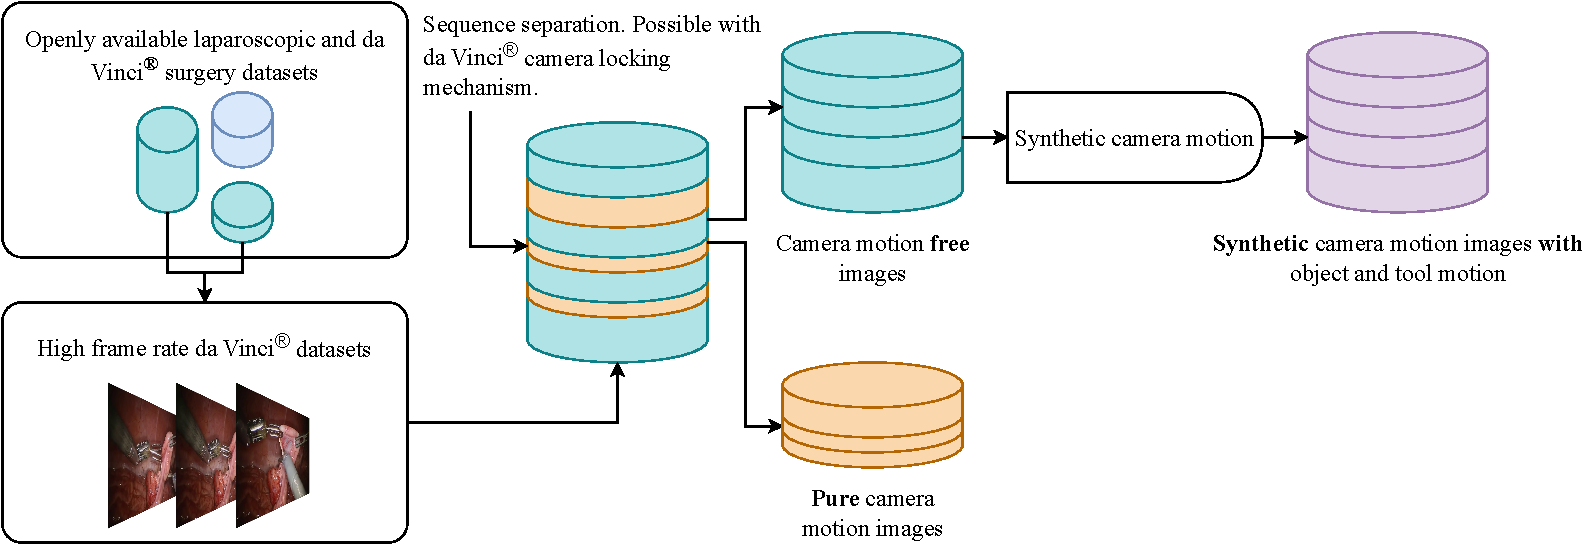
\includegraphics[width=\textwidth]{introduction/fig/camera_motion.pdf}
    \caption{The proposed isolation of camera motion, i.e. actions, and tool as well as object motion. The camera locking mechanism of the da Vinci\textsuperscript{\textregistered} robot allows for extraction of camera motion free image sequences, see \tabref{in:tab:datasets}. Synthetically added camera motion can be used for supervised training. Refers to \secref{in:sec:supervised_self_supervised}.}
    \label{in:fig:camera_motion}
\end{figure}
Paradoxically, camera motion is accessible and intrinsic to videos of laparoscopic interventions, the crux lies in extracting it reliably and isolating it from tool and object motion, for which, currently, no method exists. It is thus not surprising that existing literature on \gls{il} for camera motion automation still utilizes data from mock setups~\cite{ji2018learning,wagner2021learning}. As was discussed in \secref{in:sec:auxiliary_tasks}, so far the existing data is mainly leveraged to solve auxiliary tasks that could at best contribute to camera motion automation. In this section, we will propose a clever trick to extract camera motion from laparoscopic interventions, refer \secref{in:sec:search_for_available_data}, as a means of generating state-action pairs.

\paragraph{Extracting Camera Motion from Laparoscopic Interventions}
The state of the system $\hat{s}_t$, although underdetermined with only access to the images, see \figref{in:fig:hypothesized_pipeline}, is already known. The remaining difficulty is to extract actions from the change between subsequent states, that is extracting camera motion $\hat{a}_t$ from the subsequent states $\hat{s}_t$ and $\hat{s}_{t+1}$. As a reminder, actions lead to a change in the state, nicely shown in \figref{in:fig:reinforcement_learning}. It is difficult because it is hard to differentiate between camera, tool, and object motion. Although their might be different methods for achieving this, in this work we propose to train a neural network in a supervised fashion on isolating camera from object and tool motion. A visualization for how we are planning to achieve this is shown in \figref{in:fig:camera_motion}. In summary, we propose to use all existing data from da Vinci\textsuperscript{\textregistered} surgeries with high frame rates, see \tabref{in:tab:datasets}. Next, and as hinted in \secref{in:sec:search_for_available_data}, we manually isolate sequences with camera motion from sequences without camera motion. This is made possible by the locking system of da Vinci\textsuperscript{\textregistered} robots. Keeping in mind that the sequences without camera motion still contain object and tool motion, we suggest to add camera motion synthetically. The synthetically added camera motion can then be used to as ground truth for a neural network. We will be hypothesizing that the learned camera motion extraction will function on videos of laparoscopic interventions to generate image-action pairs.

\paragraph{Camera Motion Prediction} Assuming that a sufficiently accurate camera motion extractor can be provided through the above proposal, camera motion prediction should follow swiftly. One would simply take the extracted camera motion as a pseudo-label. This would lead to predicting image space actions $\hat{a}_t$, as these are invariant of the domain, refer \figref{in:fig:hypothesized_pipeline}, which was already proposed in \figref{in:fig:shared_domain}. The important part is that the extracted as well as the predicted camera motion should be executable on a robotic laparoscope holder. Appropriate means of describing the camera motion will be introduced in the next \secref{in:sec:homography_based_camera_motion_formulation}.

\subsubsection{Homography-based Camera Motion Formulation}
\label{in:sec:homography_based_camera_motion_formulation}
Extracting camera motion from images is a well studied problem, but not so much in the surgical context, where an extremely dynamic and deformable environment with little texture hardens the task. Therefore, simplifying the problem is crucial. In its simplest form, one can model a surgical scene as a plane, the change in observed views, i.e. induced through camera motion, can then be described via homographies. Homographies are thus a good candidate for describing actions $\hat{a}^*_t$, necessary for \figref{in:fig:hypothesized_pipeline}. They additionally can be utiliezd to feedback a control signal to the robot. In this section, we will first describe homographies and their theoretical background. Next, we will explain how they can be used to control the velocity of a camera frame C. 

% , camera motion can hence be described as a homography and recent advances in deep homography estimation have successfully extracted homographies from images with little texture~\cite{detone2016deep, erlik2017homography, nguyen2018unsupervised}. These findings were further applied in the surgical realm by Gomes et al. in~\cite{gomes2019unsupervised} and by Bano et al. in~\cite{bano2020deep}. Bano et al. further refined their findings in~\cite{bano2020vessel} by segmenting veins for the registration process. Yet, none of the above methods takes dynamic scenes into consideration. Most recent literature on deep homography estimation demonstrated how deep homography estimation can be applied to dynamic scenery~\cite{le2020deep, zhang2019content}.

\paragraph{Homographies and Four Point Representation} Two images are related by a homography if both images view the same plane from different angles and distances. Points on the plane, as observed by the camera from different angles in homogeneous coordinates $\mathbf{p}_i = \begin{bmatrix}u_i&v_i&1\end{bmatrix}^\text{T}$ are related by a projective homography $\mathbf{G}$~\cite{malis2007deeper}
\begin{equation}
    \alpha_g\mathbf{p}_i = \mathbf{G}\mathbf{p}_i^\prime.
    \label{c3:eq:proj_hom}
\end{equation}
Since the points $\mathbf{p}_i$ and $\mathbf{p}_i^\prime$ are only observed in the 2D image, depth information is lost, and the projective homography $\mathbf{G}$ can only be determined up to scale $\alpha_g$. The distinction between projective homography $\mathbf{G}$ and homography in Euclidean coordinates $\mathbf{H} = \mathbf{K}^{-1}\mathbf{G}\mathbf{K}$, with the camera intrinsics $\mathbf{K}$, is often not made for simplicity, but is nonetheless important for control purposes. The eight unknown parameters of $\mathbf{G}$ can be obtained through a set of $N\geq4$ matching points $\mathbb{P} = \{(\mathbf{p}_i, \mathbf{p}^\prime_i), i\in[0,N-1]\}$ by rearranging \eqref{c3:eq:proj_hom} into
\begin{equation}
    \begin{bmatrix}
        u^\prime_i & v^\prime_i & 1 & 0   &   0 & 0 & -u^\prime_i u_i & -v^\prime_i u_i & -u_i \\
        0   &   0 & 0 & u^\prime_i & v^\prime_i & 1 & -u^\prime_i v_i & -v^\prime_i v_i & - v_i
    \end{bmatrix}\mathbf{g}= \mathbf{0}\quad\forall i,
    \label{c3:eq:hom_lin_sys}
\end{equation}
where $\mathbf{g}$ holds the entries of $\mathbf{G}$ as a column vector. The ninth constraint, by convention, is usually to set $||\mathbf{g}||_2 = 1$. Classically, $\mathbb{P}$ is obtained through feature detectors but it may also be used as a means to parameterise the spatial transformation.
Recent deep approaches indeed set $\mathbb{P}$ as the corners of an image, and predict $\Delta \mathbf{p}_i = \mathbf{p}^\prime_i - \mathbf{p}_i$. This is also known as the four point homography $\mathbf{G}_{4\text{point}}$
\begin{equation}
    \mathbf{G}_{4\text{point}} = \begin{bmatrix}
        \Delta u_0 & \Delta v_0 \\
        \Delta u_1 & \Delta v_1 \\
        \Delta u_2 & \Delta v_2 \\
        \Delta u_3 & \Delta v_3
    \end{bmatrix},
    \label{c3:eq:4pt}
\end{equation}
which relates to $\mathbf{G}$ through \eqref{c3:eq:hom_lin_sys}, where $\mathbf{p}^\prime_i = \mathbf{p}_i + \Delta \mathbf{p}_i$.    

\paragraph{Relation to Camera Frame Velocity} Given a projective homography $\mathbf{G}$ in image space, a camera body frame velocity that seeks to minimize $\Delta \mathbf{p}_i$ can be derived \`{a} la~\cite{benhimane2006homography}. 

Be $\mathbf{x}^\prime = \begin{bmatrix}
    x^\prime & y^\prime & z^\prime
\end{bmatrix}^T$ a point in 3D coordinates  and its observation under a homography transform $\mathbf{H}$:
\begin{equation}
    \mathbf{x} = \mathbf{H}\mathbf{x}^\prime. 
\end{equation}
In normalized coordinates $\mathbf{m}^\prime = \frac{1}{z^\prime} \mathbf{x}^\prime$ we get
\begin{equation}
    \frac{z}{z^\prime}\mathbf{m} = \mathbf{H} \mathbf{m}^\prime.
\end{equation}
It can then be shown that a translational error $^\text{C}\mathbf{e}_v$ and a rotational error $\left[^\text{C}\mathbf{e}_\omega\right]_\times$ exist that yield camera body frame velocities which locally converge $\mathbf{m} \rightarrow \mathbf{m}^\prime$. These can be expressed through
 \begin{equation}
    \begin{split}
        ^\text{C}\mathbf{e}_v & = (\mathbf{H} - \mathbf{I})^{\text{C}^\prime}\mathbf{m}^\prime\\
        \left[^\text{C}\mathbf{e}_\omega\right]_\times & = \mathbf{H} - \mathbf{H}^\text{T}.
    \end{split}
    \label{in:eq:dc}
\end{equation}


% theoretical background homography estimation paper

% create the bridge to execution on robot, refer to \secref{in:sec:camera_intrinsic_calibration} for intrinsics

% introduce all the deep homography estimation here, that is related work??? maybe not hu, na dont introduce this crap here, as already in papers

% needs to comply with image + robot

% deformable... assuming the scene is a plane in the first instance, add the text that was writting but commented out above

% embodying domain-irrelevant actions
% extracting actions
% predicting actions

\subsubsection{Robotic Laparoscope Control}
\label{in:sec:robotic_laparoscope_control}
Given the relation between image space action and camera frame velocity that was introduced in the above \secref{in:sec:homography_based_camera_motion_formulation}, only a mapping from camera frame velocity to joint space velocity $\dot{\mathbf{q}}$ is missing for controlling a robotic laparoscope holder. To this end we assume that the transformation from robot end-effector to camera frame $\homogeneous{E}{C}$ is accurately known. This can e.g. be achieved through the methods described in \secref{in:sec:camera_intrinsic_calibration} and \secref{in:sec:eye_in_to_hand_calibration}. Given the kinematics of the serial manipulator and the homogeneous transform end-effector to camera $\homogeneous{E}{C}$, a relation between joint velocties $\dot{\mathbf{q}}$ and camera frame velocity ${}^B\dot{\mathbf{x}}_C$ can be established through the Jacobian matrix $\mathbf{J}$ as follows
\begin{equation}
    {}^B\dot{\mathbf{x}}_C = \mathbf{J} \dot{\mathbf{q}}.
\end{equation}
The Jacobian therein can be determined analytically through geometrical considerations. Inverting this locally linear equation yields target joint velocities
\begin{equation}
    \dot{\mathbf{q}} = \mathbf{J}^{\dagger}{}^B\dot{\mathbf{x}}_C.
    \label{in:eq:jacobian_inverse}
\end{equation}
This relation may e.g. be used in a \gls{pid} control scheme. The exact use of \eqref{in:eq:jacobian_inverse} to control a camera frame body velocity through \eqref{in:eq:dc} with additional \gls{rcm} constraint will further be contributed as part of \chapref{chap:robotic_endoscope} in \secref{c2:sec:methods}.

% that is associated with blablablabla

%\gls{rcm} ? maybe just jacobian should be fine

% give a good explanation for the relation of camera frame velocity with joint velocity mapping, camrea intrinsic parameters etc, so that the derivation of rcm can still be kept for chapter visual servoing

% theory of control paper up to merge, i.e. no including merge of two methods

% \subsection{Minimally Invasive Surgery}
% Minimally Invasive Surgery (MIS) minimizes blood loss, allows for faster recovery and leaves a patient with smaller scars. In traditional MIS, a main surgeon would usually be supported by an assistant to help move the endoscope. In this setup, the assistant surgeon often introduces tremor and suffers fatigue. To oveRCMe these, robotic endoscope holders like AESOP~\cite{unger1994aesop} or EndoAssist~\cite{gilbert2009endoassist} were developed. Different control schemes, such as gaze control, control via joystick, foot or voice were investigated. They, however, lead to eye strain, additional mental workload or communication failures, respectively. Therefore, attempts to automate the endoscope motion via visual servoing were explored. These can broadly by separated into approaches that rely on a mechanical remote center of motion (\gls{rcm}) and approaches that cast the \gls{rcm} as part of the optimal control, often referred to as programmable \gls{rcm}. 




% \subsection{Imitation Learning in this Work}
% Given the advancements in deep learning and especially in \gls{il}, it seems surprising that no one applied \gls{il} to automate camera motion in laparoscopic surgery. After having a closer look, it comes, however, at no wonder people have not tried. Three major challenges reside:
% \\
% \begin{itemize}
% 	\item \gls{il} requires big data, but data collection is expensive, especially in realistic setups. The only two publicly available datasets that come with kinematic labels are MISAW~\cite{mitsuishi2013master} and JIGSAW~\cite{ahmidi2017dataset}, but both datasets are captured in a synthetic environment and without camera motion. This results in the challenge that all of the available data has no camera motion action labels, and reliably extracting camera motion in retrospect from dynamic surgical scenery is an unsolved task in itself.
% 	\item There exists an unknown domain shift between laparoscopic surgery data and the robotic system. This domain shift could be gapped via Reinforcement Learning (RL) on top of \gls{irl}, but simple RL in the medical realm puts the patient at risk. We gap this domain shift by finding the greatest common divisor between human demonstrator and robotic learner with a novel optimal control formulation.
% 	\item From the available data, neither the goal state nor the reward function are apparent. Simple \gls{bc} under a noisy action estimation might be too difficult. To imitate a surgeon demonstrator, a proxy for good views has to be found.\\
% \end{itemize}
% In the following we address how to tackle the first and second challenge. We further identify pathways to solve the third task.

% \section{METHODS}
% In this section, we first introduce a composite Jacobian gain controller with \gls{rcm} objective in \secref{in:sec:task_RCM}. We then introduce a homography-based visual servo task for the latter in \secref{in:sec:visual_servo}. Finally, in \secref{in:sec:homography_regression}, we describe different ways of extracting homographies from images.
% \subsection{Task Control with Remote Center of Motion}
% \label{in:sec:task_RCM}
% As derived in~\cite{aghakhani2013task}, we update the robot's joint velocities $\dot{\mathbf{q}}$ with a gain controller, following \eqref{in:eq:gain_controller}
% \begin{equation}
% 	\begin{bmatrix}
% 		\dot{\mathbf{q}} \\ 
% 		\dot{\lambda}
% 	\end{bmatrix} =
% 	\mathbf{J}^\#
% 	\begin{bmatrix}
% 		\mathbf{K}_\text{t} & \mathbf{0}_{\text{n}_\text{t} \times 3} \\
% 		\mathbf{0}_{3\times \text{n}_\text{t}} & \mathbf{K}_\text{RCM}
% 	\end{bmatrix}\mathbf{e},
% 	\label{in:eq:gain_controller}
% \end{equation}
% where $\dot{\lambda}$ describes the relative change of the \gls{rcm} along the endoscope, $\mathbf{J}^\#$ denotes the pseudo-inverse of the composite Jacobian, and $\mathbf{K}_\text{t}$, and $\mathbf{K}_\text{RCM}$ are the gains for the task, and the \gls{rcm}, respectively. The error $\mathbf{e}$ is defined as
% \begin{equation}
% 	\mathbf{e} = 
% 	\begin{bmatrix}
% 		\mathbf{e}_\text{t} \\
% 		\mathbf{p}_\text{trocar} - \mathbf{p}_\text{RCM}
% 	\end{bmatrix},
% 	\label{in:eq:error}
% \end{equation}
% with the desired trocar position $\mathbf{p}_\text{trocar}$, and the current \gls{rcm} position $\mathbf{p}_\text{RCM}$ under the relative position $\lambda$. We keep an internal state for the relative position of the \gls{rcm} $\lambda$ and update it via the desired trocar position $\mathbf{p}_\text{trocar}$ as follows
% \begin{equation}
% \lambda = \frac{(\mathbf{p}_{i+1} - \mathbf{p}_i)^T(\mathbf{p}_\text{trocar}-\mathbf{p}_i)}{\lVert\mathbf{p}_{i+1} - \mathbf{p}_i\rVert_2^2}
% \end{equation}
% Therein, $\mathbf{p}_{i+1}$ denotes the position of the end-effector, which coincides with the camera frame up to orientation and $\mathbf{p}_i$ denotes the joint position prior to the end-effector.
% \subsection{Homography-based Visual Servo Task}
% \label{in:sec:visual_servo}
% As the task error $\mathbf{e}_\text{t}$ in \eqref{in:eq:error}, we use the twist of the camera frame, expressed in the camera frame. Therefore, we rotate the twist from the camera frame to the world frame using $^\textbf{w}\mathbf{R}_\textbf{c}$, as shown below
% \begin{equation}
% 	\mathbf{e}_\text{t} = 
% 	\begin{bmatrix}
% 		^\textbf{w}\mathbf{R}_\textbf{c} & \mathbf{0}_{3\times 3} \\
% 		\mathbf{0}_{3\times 3} & ^\textbf{w}\mathbf{R}_\textbf{c}
% 	\end{bmatrix}
% 	\begin{bmatrix}
% 		\mathbf{e}_{v} \\
% 		\mathbf{e}_\omega
% 	\end{bmatrix}.
% 	\label{in:eq:task}
% \end{equation}
% Following~\cite{benhimane2006homography}, we then compute the twist $\begin{bmatrix}\mathbf{e}_v & \mathbf{e}_\omega\end{bmatrix}^T$ from
% \begin{equation}
% 	\begin{split}
% 		\mathbf{e}_v = (\mathbf{H} - \mathbf{I})\mathbf{m}^*\\
% 		[\mathbf{e}_\omega]_\times = \mathbf{H} - \mathbf{H}^T,
% 	\end{split}
% 	\label{in:eq:twist}
% \end{equation}
% where $\mathbf{H}$ is the homography from the desired to the current frame and $\mathbf{m}^*=\begin{bmatrix}
% x^* & y^* & 1
% \end{bmatrix}$ is set as the principal point, hence $\mathbf{m}^* = \mathbf{K}^{-1}\mathbf{p}^*$, with the camera intrinsics $\mathbf{K}$ and $\mathbf{p}^* = \begin{bmatrix}
% u^* & v^* & 1
% \end{bmatrix}$, the principal point in image space.
% \subsection{Homography Regression}
% \label{in:sec:homography_regression}
% Homographies $\mathbf{H}$ express the transformation of points on a plane, which are projected onto normalized coordinates, under rotation and translation of the camera reference frame. Hence one can write
% \begin{equation}
% 	\mathbf{H}\mathbf{m} = \mathbf{m}'
% 	\label{in:eq:homography}
% \end{equation}
% An unknown homography can be found by identifying a set of point correspondences $\{\mathbf{m}_i, \mathbf{m}'_i\}$. By rearranging \eqref{in:eq:homography}, one can define a set of linear equations as follows
% \begin{equation}
% 	\begin{bmatrix}
% 		x_i & y_i & 1 &   0 &   0 & 0 & -x_ix'_i & -y_ix'_i & -x'_i \\
% 		  0 &   0 & 0 & x_i & y_i & 1 & -x_iy'_i & -y_iy'_i & -y'_i
% 	\end{bmatrix}\mathbf{h} = \mathbf{0},
% 	\label{in:eq:homography_linear}
% \end{equation}
% where $\mathbf{h}$ is a column vector holding the entries of $\mathbf{H}$. Since $\mathbf{H}$ is defined up to scale, it has $8$ unknown parameters. Each point $\mathbf{m}_i$ has $2$ variables, it is thus sufficient to find $4$ point correspondences to solve \eqref{in:eq:homography_linear}. Since the points $\mathbf{m}_i$ are usually found in image space $\mathbf{p}_i$, one obtains the projective homography $\mathbf{G}$ by simply solving the equivalent of \eqref{in:eq:homography_linear}. It can be transferred to normalized coordinates via the camera intrinsics $\mathbf{K}$ with
% \begin{equation}
% \mathbf{H} = \mathbf{K}^{-1}\mathbf{G}\mathbf{K}.
% \end{equation}
% A common way to find a set of point correspondences $\{\mathbf{p}_i, \mathbf{p}'_i\}$ in the image space is to find feature descriptors using for example the Scale-invariant Feature Transform (SIFT)~\cite{lindeberg2012scale} or Speeded-up Robust Features (SURF)~\cite{bay2006surf} and to identify nearest neighbors within the feature descriptors. Another way, subject to more recent research, is to directly learn $\Delta\mathbf{p}_i = \mathbf{p}_i - \mathbf{p}'_i$, the deviation of image edges under a homography transformation, from image space~\cite{detone2016deep}. This can be achieved with a neural network, since the homography in \eqref{in:eq:homography_linear} can be differentiated with respect to the set of points $\{\mathbf{p}_i, \mathbf{p}'_i\}$. 
% \subsection{Implementation - Visual Servo with \gls{rcm}}
% We implement the gain controller from \eqref{in:eq:gain_controller}, as well as the visual servo from \eqref{in:eq:twist}, with the linear algebra library Eigen~\cite{guennebaud2010eigen}. Hereby, we obtain the Jacobian matrices in \eqref{in:eq:gain_controller} and the rotations in \eqref{in:eq:task} with the MoveIt library~\cite{chitta2012moveit}. To suppress singular forces, we compute the pseudo-inverse of the task Jacobian $\mathbf{J}$ via a damped least-squares solution using the Singular Value Decomposition~\cite{buss2004introduction}. To ensure safety, we implement the gain controller as an action server within the Robot Operating System (ROS)~\cite{quigley2009ros} that only allows the execution of non-converging joint velocities $\dot{\mathbf{q}}$.
% \subsection{Implementation - Homography Regression}
% \label{in:sec:implementation_homography_regression}
% We synthetically generate image data. Therefore, we randomly augment fog, grayscale, flipping (horizontally and vertically), blurring, brightness and contrast operations.

% \begin{figure}[htb]
% 	\centering
% 	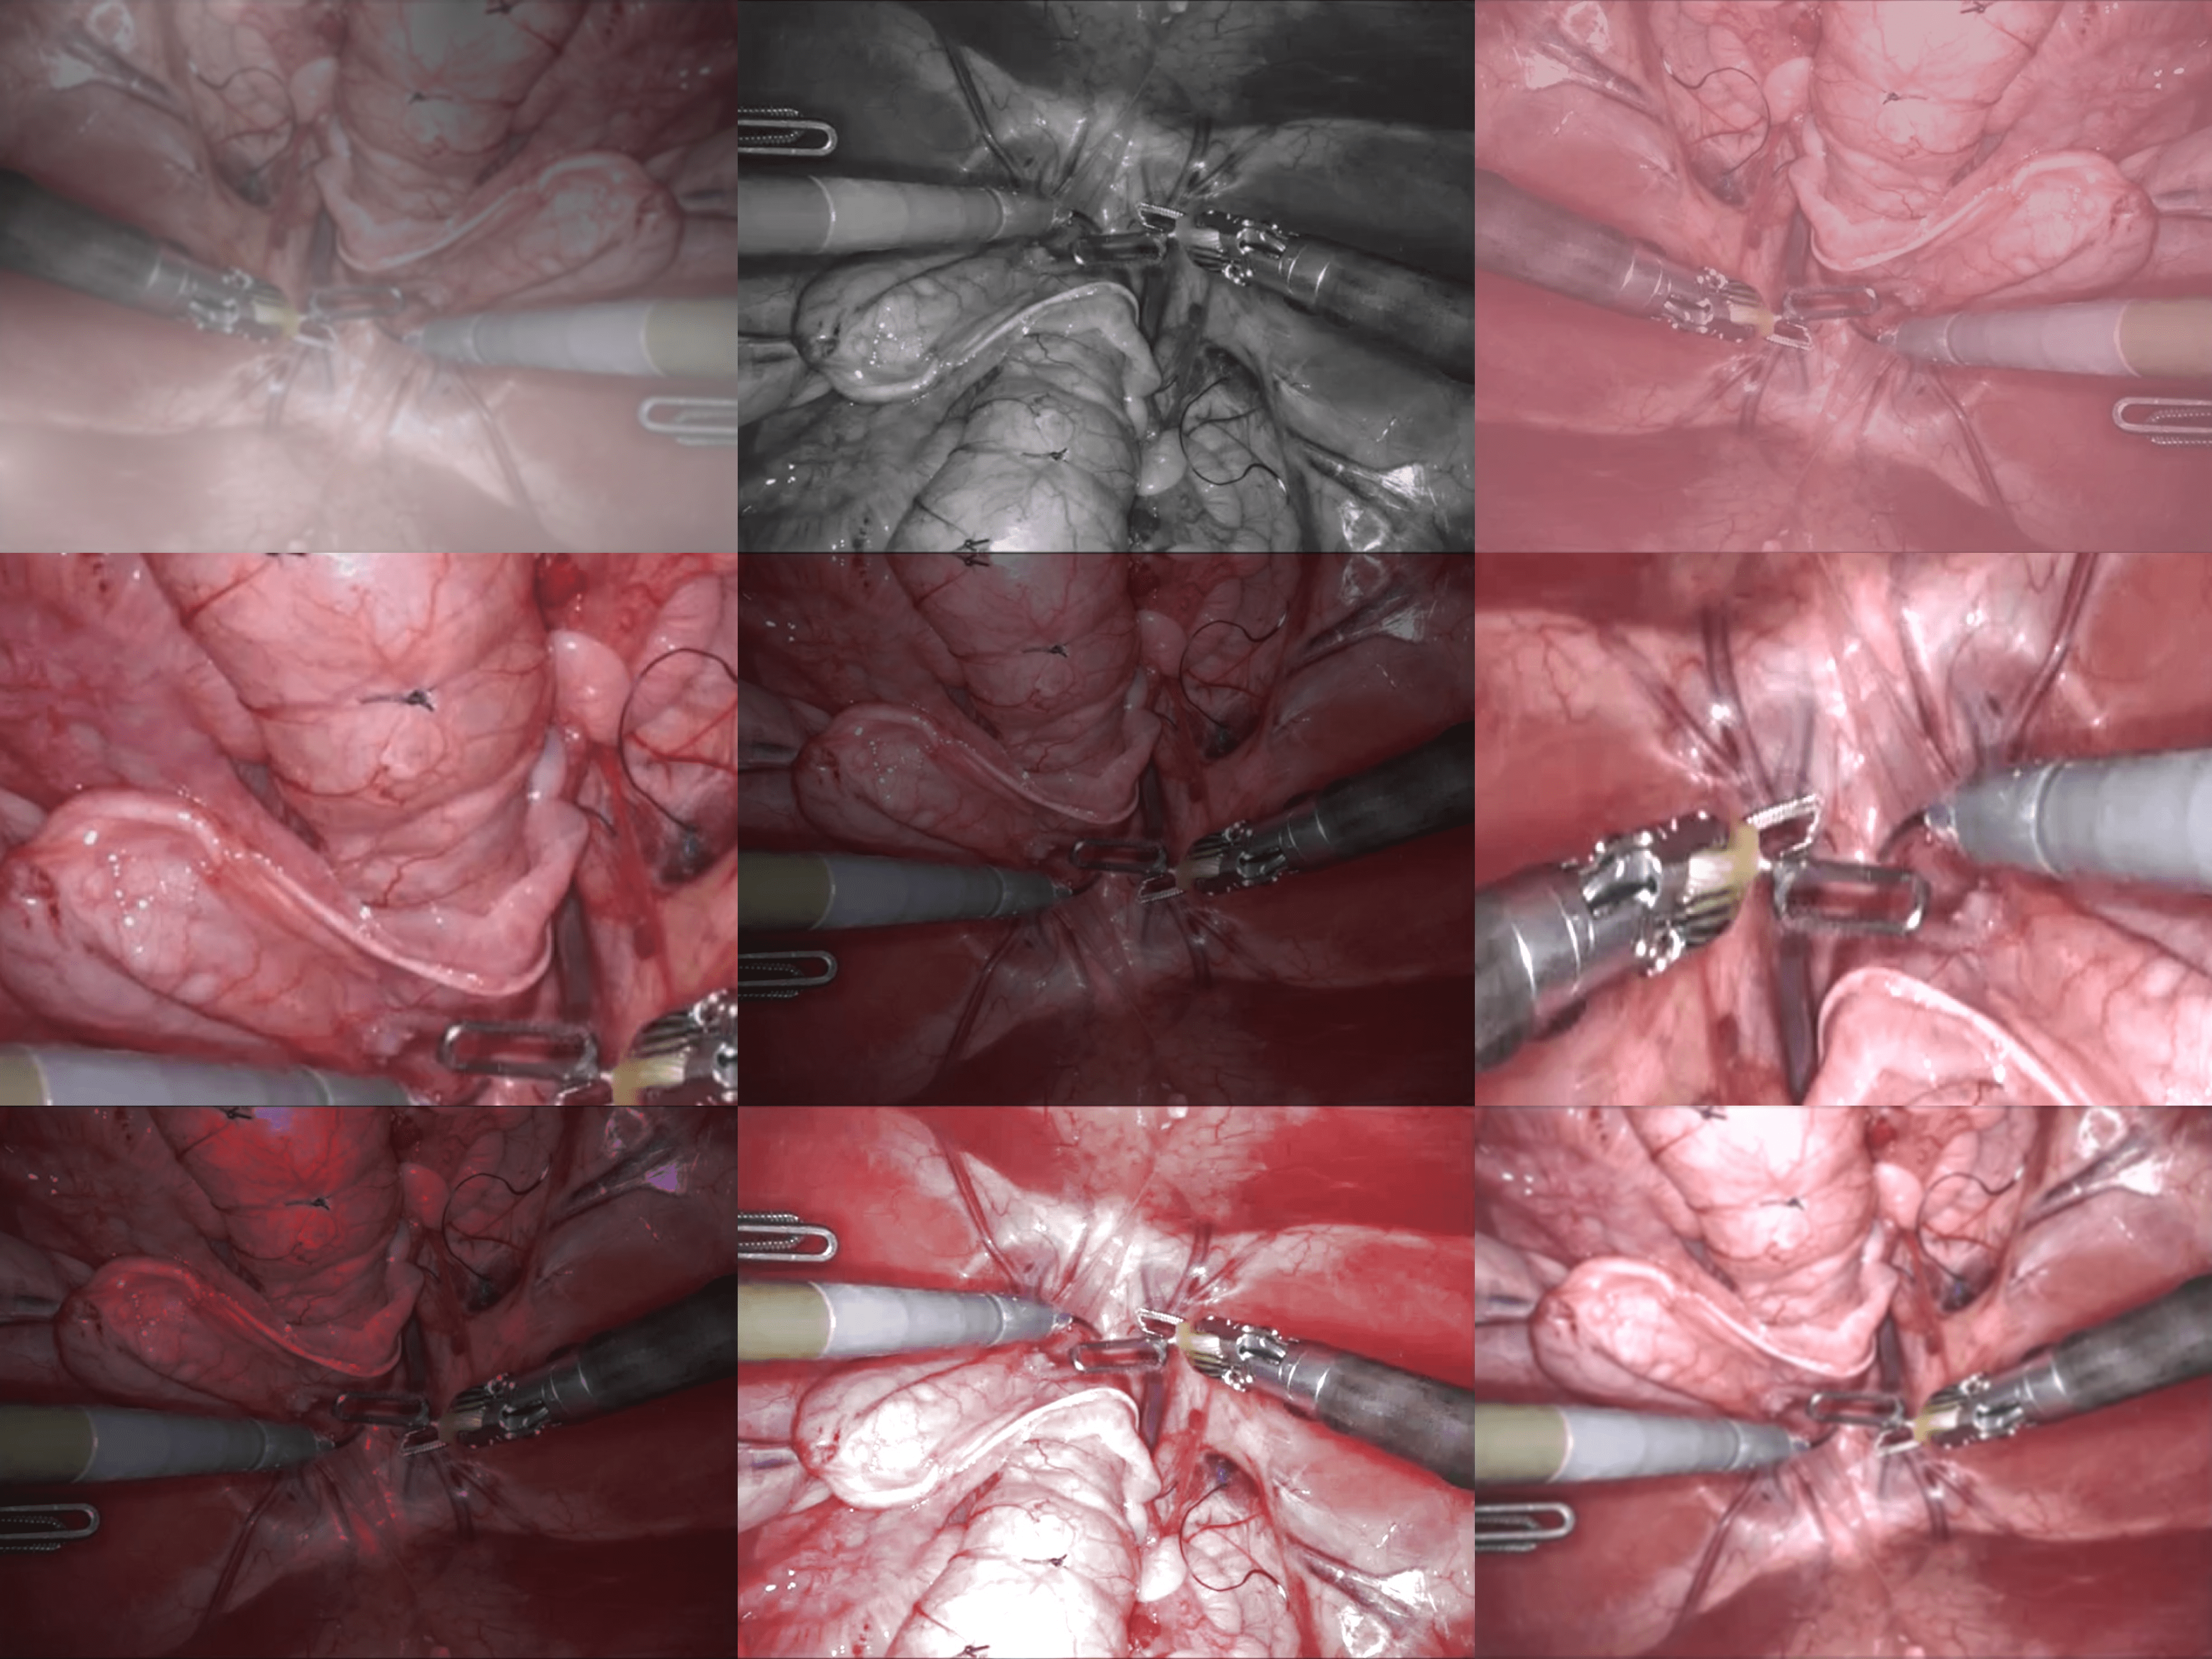
\includegraphics[width=0.8\textwidth]{img/compresspng/augmentations.png}
% 	\caption{Nine different sample variations of the same image from the da Vinci\textsuperscript{\textregistered} SurgVisDom dataset. Shown are random combinations of fog, grayscale, flip, blur, brightness, contrast and crop augmentations.} 	
% 	\label{in:fig:data_augmentation}
% \end{figure}

% As in~\cite{detone2016deep}, we then crop the augmented image at edges $\{\mathbf{p}_i\}$, which we then deviate by $\{\Delta \mathbf{p}_i\}$. We apply the corresponding inverse homography to the full image and test whether all points $\{\mathbf{p}_i\}$ still reside within the polygon that is spanned by the new image edges. If so, we keep the sample $\{\mathbf{I}^\text{crop}_t, \mathbf{I}^\text{crop, warp}_{t+1}, \{\Delta\mathbf{p}_i\}\}$ as data point, else we resample $\{\Delta \mathbf{p}_i\}$. To regress $\{\Delta\mathbf{p}_i\}$ in between the sample $\{\mathbf{I}^\text{crop}_t, \mathbf{I}^\text{crop, warp}_{t+N}\}$, we further forward the image pair through a neural network and implement \eqref{in:eq:homography_linear} with the differentiable computer vision library Kornia~\cite{riba2020kornia}. As DeTone et al. in~\cite{detone2016deep}, we do this in a supervised manner, where we directly regress $\{\Delta\mathbf{p}_i\}$, however, as Nguyen et al. in~\cite{nguyen2018unsupervised} and Zhang et al. in~\cite{zhang2019content}, we further compute the loss in the image space on the tuple $\{\mathbf{I}^\text{crop}_t, \mathbf{I}^\text{crop, warp}_{t+N}\}$ in an unsupervised approach.
% \subsection{Experimental Setup}
% In our experimental setup, see \figref{in:fig:experimental_setup}, we use a  KUKA \gls{lbr} Med 7 R800 robot. To control it, we create a bridge to ROS by wrapping the Fast Robot Interface (FRI)~\cite{schreiber2010fast} with ROS' Hardware Interface functionality. We mount the laparoscope to the \gls{lbr} Med 7 robot with a custom designed 3D print. As the laparoscope, we use a Storz 7230 AA Telescope, from which we capture images using a Storz TH 102 H3-Z FI Camera. For illumination, we additionally connect a Storz TL 300 Power LED 300 light source to the laparoscope. The acquired images are sent to the Storz TC 300 Image1 S H3-Link, which links the camera via DP to the Storz TC 200 Image1 S Connect. From there on, the image feed is output to SDI, which we convert to HDMI with a SDI to HDMI converter. We then grab the HDMI signal with a DeckLink 4K Extreme 12G and stream it onto the ROS network.

% \subsection{Data}
% To facilitate imitation learning on laparoscopic surgery data, we extract and isolate camera motion from object motion. Therefore, we collect da Vinci\textsuperscript{\textregistered} surgery data, where the camera only moves occasionally and is mostly fixed in position, but objects are still moving. We isolate data without camera motion from data with camera motion. We additionally collect laparoscopic surgery data with camera motion to imitate it. An exhaustive overview of publicly available datasets is given in \tabref{in:tab:datasets}. We analyze the data for its length, frame rate, resolution and camera motion. We pre-process the laparoscopic data by searching for its center point and bounding circle. We do so by seeking a circle who's radius and center fit best to the edge filtered laparoscopic view with a random sample consensus (RANSAC)~\cite{fischler1981random}, see \figref{in:fig:ransac_circle}.

% \begin{figure}[htb]
% 	\centering
% 	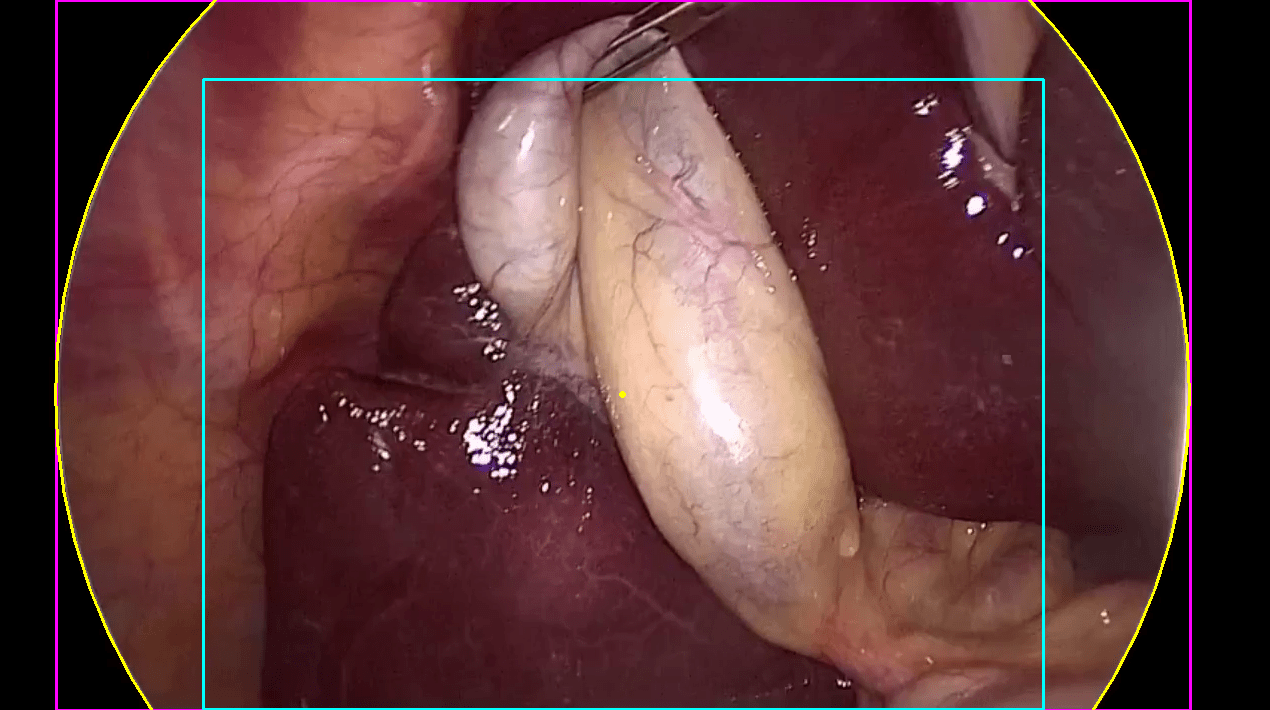
\includegraphics[width=0.8\textwidth]{img/compresspng/ransac_0.png}
% 	\caption{RANSAC detection of the circular boundary of the laparoscopic image from Cholec80~\cite{twinanda2016endonet} (yellow). The turquoise rectangle is the maximum sized rectangle of a given aspect ratio that fits around the circle's center point. An example \href{https://drive.google.com/file/d/1aY7jnBoKNwKyMlSthjzgsRldkHEK1OKw/view?usp=sharing}{video} is provided.}
% 	\label{in:fig:ransac_circle}
% \end{figure}

% \begin{landscape}
% \begin{table}[htb]
% \centering
% \caption{Exhaustive overview of publicly available \gls{mis} datasets. All datasets were acquired and analyzed for task-appropriate metrics. in:tab:datasetsMetrics were marked with N/A, where datasets were not available or unreasonable to analyze.}
% \label{in:tab:datasets}
%     \begin{tabular}{|c|c|c|r|c|c|c|c|}
%         \hline
%         \multirow{2}{*}{Collection} & \multicolumn{7}{c|}{Specifications} \\
%         \cline{2-8}
%         & Name & Year & Length / \# & Frame Rate / Hz & Resolution / pixels & Camera Motion & Note \\
%         \hline
%         \multirow{8}{*}{\href{https://endovis.grand-challenge.org/}{\shortstack{Endoscopic\\Vision\\Challenge}}} &\href{https://www.synapse.org/#!Synapse:syn21776936/wiki/601700}{MISAW}~\cite{mitsuishi2013master}&2020&$128102$&$30$&$460\times 540$&no&synthetic \\
%         \cline{2-8}
%         &\href{https://surgvisdom.grand-challenge.org/}{SurgVisDom}\cite{zia2021surgical}&2020&$185620$&$20$&$540\times960$&occasional&da Vinci\textsuperscript{\textregistered} \\
%         \cline{2-8}
%         &\href{https://robustmis2019.grand-challenge.org/}{ROBUST-\gls{mis}}~\cite{maier2020heidelberg}\cite{ross2020robust}&2019&$7546968$&$25$&$540\times 960$&yes&laparoscopic \\
%         \cline{2-8}
%         &\href{https://endovissub2019-scared.grand-challenge.org/}{SCARED}&2019&$16818$&$25$&$1024 \times 1280$&yes& exoscopic \\
%         \cline{2-8}
%         &\href{https://endovissub-workflowandskill.grand-challenge.org/}{SWASA}&2019&N/A&N/A&N/A&yes& laparoscopic\\
%         \cline{2-8}
%         &\href{https://endovissub2017-workflow.grand-challenge.org/}{SWASA}&2018&N/A&N/A&N/A&yes& laparoscopic\\
%         \cline{2-8}
%         &\href{https://endovissub2018-roboticscenesegmentation.grand-challenge.org/home/}{RSS}~\cite{allan20202018}&2018&$2235$&$2$&$1024\times 1280$&occasional& da Vinci\textsuperscript{\textregistered}\\
%         \cline{2-8}
%         &\href{https://endovissub2017-roboticinstrumentsegmentation.grand-challenge.org/}{RIS}~\cite{allan20192017}&2017&$3225$&$2$&$1024\times 1280$&occasional& da Vinci\textsuperscript{\textregistered} \\
%         \cline{2-8}
%         &\href{https://endovissub2017-kidneyboundarydetection.grand-challenge.org/}{KBD}&2017&$3000$&$2$&$1024\times 1280$&occasional & da Vinci\textsuperscript{\textregistered}\\
%         \cline{2-8}
%         &\href{https://endovissub-instrument.grand-challenge.org/}{ISAT}&2015&$16243$&$25$&$480\times 640/576\times 720$& yes & laparoscopic \\
%         \hline
%         \multirow{3}{*}{\href{http://hamlyn.doc.ic.ac.uk/vision/}{\shortstack{Hamlyn\\Center\\Datasets}}} &\href{http://hamlyn.doc.ic.ac.uk/vision/data/daVinci.zip}{Siamese}\cite{ye2017self}&2017&$34240$&$30$&$192\times 384$& occasional& da Vinci\textsuperscript{\textregistered} \\
%         \cline{2-8}
%         &Giannarou \href{http://hamlyn.doc.ic.ac.uk/vision/data/Matina/Blur/capture1.avi}{left} / \href{http://hamlyn.doc.ic.ac.uk/vision/data/Matina/Blur/capture2.avi}{right}~\cite{giannarou2012probabilistic}&2012&$8063$&$30$&$480\times 640$& occasional& da Vinci\textsuperscript{\textregistered} \\ 
%         \cline{2-8}
%         &Mountney \href{http://hamlyn.doc.ic.ac.uk/vision/data/Dataset8/left.avi}{left} / \href{http://hamlyn.doc.ic.ac.uk/vision/data/Dataset8/right.avi}{right}~\cite{mountney2010three}&2010&$14418$&$30$&$480\times 640$& occasional & da Vinci\textsuperscript{\textregistered}\\
%         \hline
%         \multirow{4}{*}{Other} &\href{https://www.youtube.com/}{YouTube}&N/A&N/A&N/A&N/A&N/A & N/A \\
%         \cline{2-8}
%         &\href{https://saras-esad.grand-challenge.org/}{SARAS-ESAD}~\cite{bawa2020esad}&2020&$18793$&$1$&$1080\times 1920$& occasional & da Vinci\textsuperscript{\textregistered} \\
%         \cline{2-8}
%         &\href{http://camma.u-strasbg.fr/datasets}{Cholec80}~\cite{twinanda2016endonet}&2017&$4612530$&$25$&$480\times 854$&yes& laparoscopic\\
%         \cline{2-8}
%         &\href{https://cirl.lcsr.jhu.edu/research/hmm/datasets/jigsaws_release/}{JIGSAW}~\cite{ahmidi2017dataset}&2016&$527491$&$30$&$480\times 640$&no& synthetic\\
%         \hline
%     \end{tabular}
% \end{table}
% \end{landscape}

% \section{RESULTS}
% In this section we first present and evaluate results for the visual servo in simulation in \secref{in:sec:results_visual_servo} and following that we analyze the homography regression performance in \secref{in:sec:results_homography_regression}. Finally, we measure the homography regression performance qualitatively in a dynamic surgical scene from a previously unseen dataset in \secref{in:sec:homography_imitation_learning}
% \subsection{Homography-based Visual Servo with \gls{rcm} Objective}
% \label{in:sec:results_visual_servo}
% To demonstrate the effectiveness of the proposed visual servo, we implement an example, where the desired homography $\mathbf{H}$ is computed as a least squares solution with OpenCV's \textit{findHomography} function~\cite{bradski2000opencv}. We extract key points from a calibration pattern, perturb the endoscope's position randomly and then iterate \eqref{in:eq:gain_controller} to minimize the task error $\mathbf{e}_\text{t}$ in \eqref{in:eq:error}, which is supposed to move the endoscope to the initial position. We set the task gain parameters $\mathbf{K}_\text{t} = \text{diag}(1.0,1.0,1.0,0.04,0.04,0.04)$ and the \gls{rcm} gain parameters $\mathbf{K}_\text{RCM} = \text{diag}(100.0, 100.0, 100.0)$. We set the damping factor for the damped least squares inverse of the Jacobian matrix to $\gamma = 0.05$.
% An exemplary \href{https://drive.google.com/file/d/1xrPTe7FdxZiUFySA3CxLsW-lJGgMdrcS/view?usp=sharing}{video} is available on Google Drive. We evaluated the convergence of the task error $\mathbf{e}_\text{t}$, the deviation of the \gls{rcm} $\mathbf{p}_\text{RCM}$ from the desired trocar position $\mathbf{p}_\text{trocar}$, as well as a visual error that we define as the mean pairwise distance of the key points found on the calibration board and the deviation of the tip position from the initial pose. Results are shown in \figref{in:fig:visual_servo_measurements}.

% \begin{figure}[htb]
% 	\centering
% 	\begin{subfigure}[b]{.4\textwidth}
% 		\centering
% 		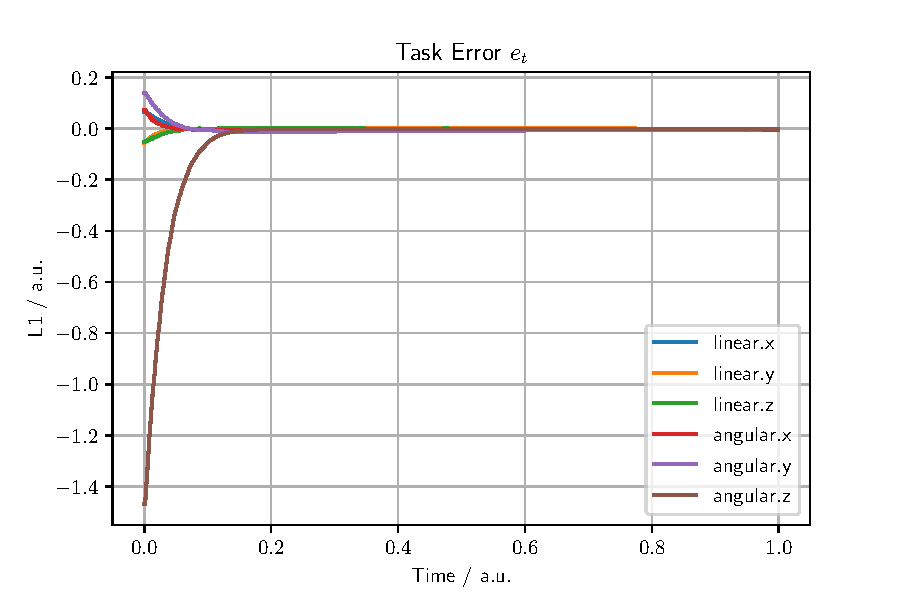
\includegraphics[width=1.0\textwidth]{fig/task_error.pdf}
% 		\caption{Task error over time, refer to \eqref{in:eq:task}. The task, as computed from the desired homography, converges.}
% 	\end{subfigure}\hspace{2em}
% 	\begin{subfigure}[b]{.4\textwidth}
% 		\centering
% 		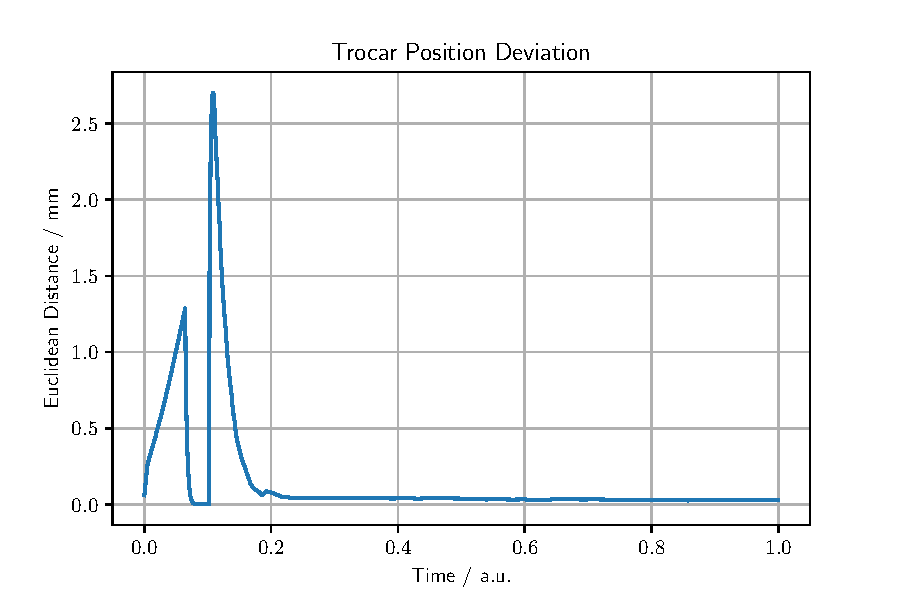
\includegraphics[width=1.0\textwidth]{fig/trocar_position_deviation.pdf}
% 		\caption{Trocar position deviation over time, refer to \eqref{in:eq:error}. The deviation stays below a couple of millimeters under task motion and converges again.}
% 	\end{subfigure}
% 	\begin{subfigure}[b]{.4\textwidth}
% 		\centering
% 		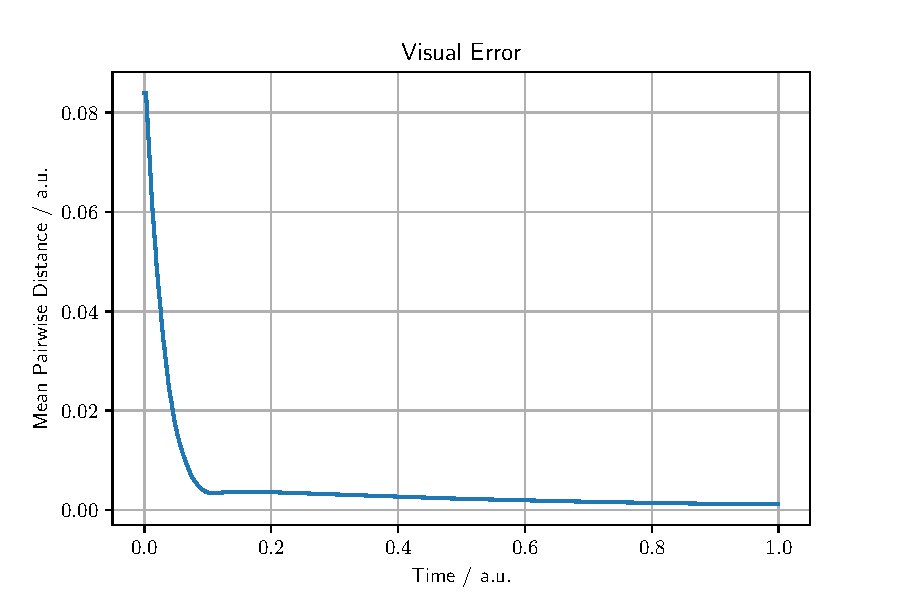
\includegraphics[width=1.0\textwidth]{fig/visual_error.pdf}
% 		\caption{The mean pairwise distance of calibration plane points in the normalized image plane converges.}
% 	\end{subfigure}\hspace{2em}
% 	\begin{subfigure}[b]{.4\textwidth}
% 		\centering
% 		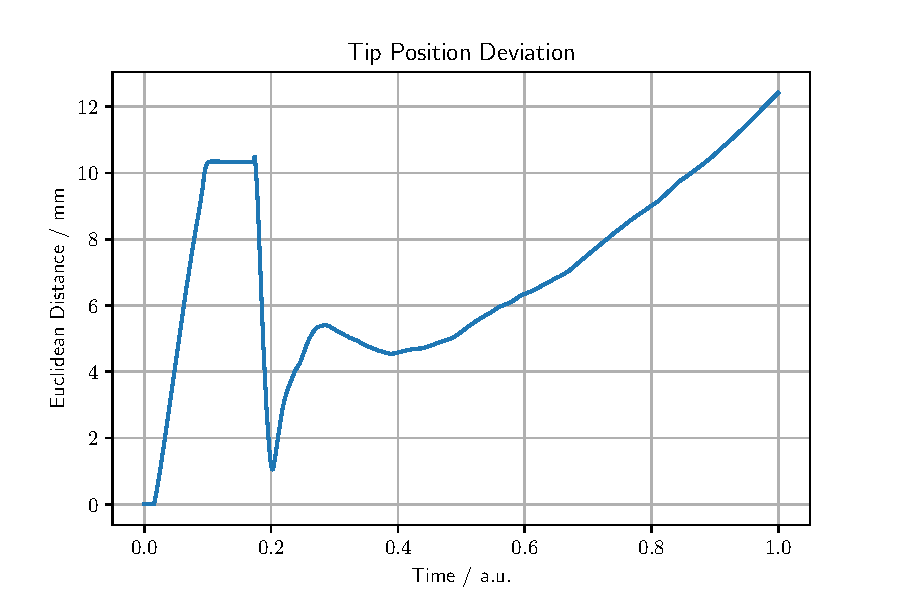
\includegraphics[width=1.0\textwidth]{fig/tip_position_deviation.pdf}
% 		\caption{The tip position is first changed on purpose, then converges to close to zero after the visual servo is initialized but then starts to diverge, although the task errors are being minimized.}
% 	\end{subfigure}
% 	\caption{Evolution of different errors over time. In the setup, we perturb the laparoscope's tip and then initialize the homography-based visual servo to return to the initial position. Results were obtained in simulation.}
% 	\label{in:fig:visual_servo_measurements}
% \end{figure}

% \subsection{Homography Regression}
% \label{in:sec:results_homography_regression}
% As visualized in \figref{in:fig:datasets_sizes}, the datasets SurgVisDom, Giannarou and Mountney account for $72.4\%$ of data with occasional camera motion. 

% \begin{figure}[htb]
% 	\centering
% 	\begin{subfigure}[b]{.45\textwidth}
% 		\centering
% 		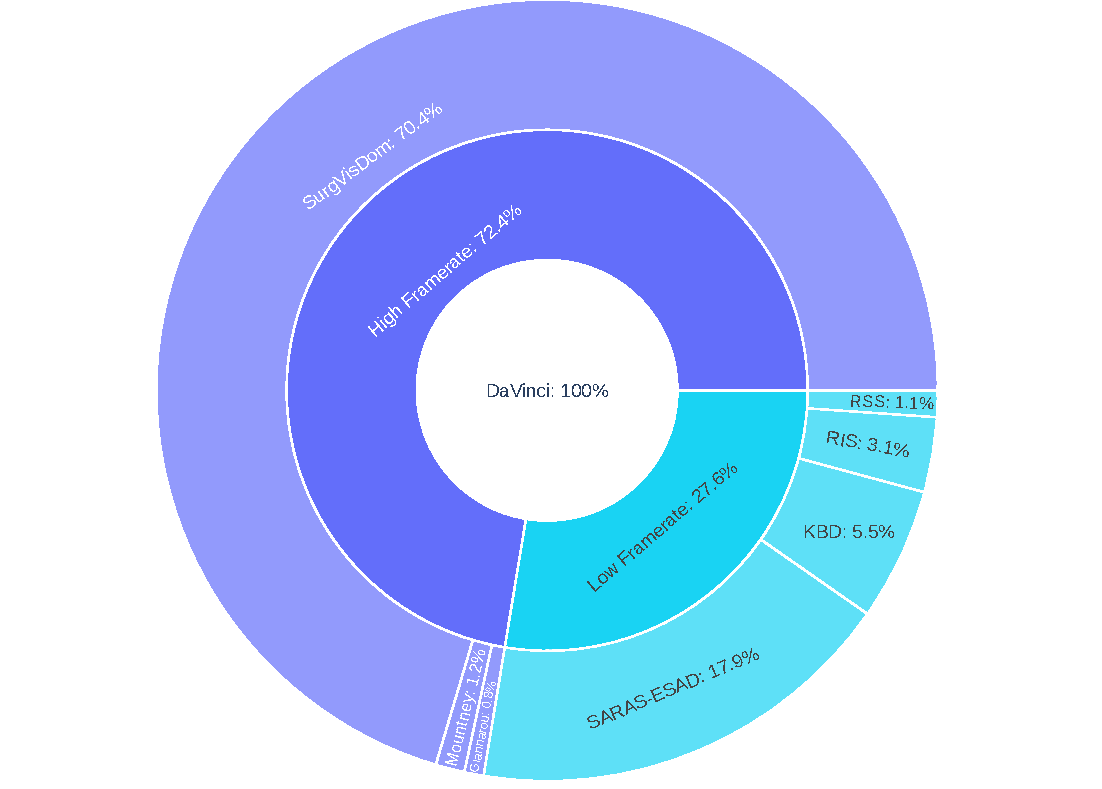
\includegraphics[width=1.\linewidth]{fig/fig_da_vinci.pdf}
% 		\caption{da Vinci\textsuperscript{\textregistered} surgery datasets modulo the Siamese dataset due to low resolution. The high frame rate datasets naturally cover $72.4\%$ of available data.}
% 		\label{in:fig:da_vinci}
% 	\end{subfigure}\hspace{2em}
% 	\begin{subfigure}[b]{.45\textwidth}
% 		\centering
% 		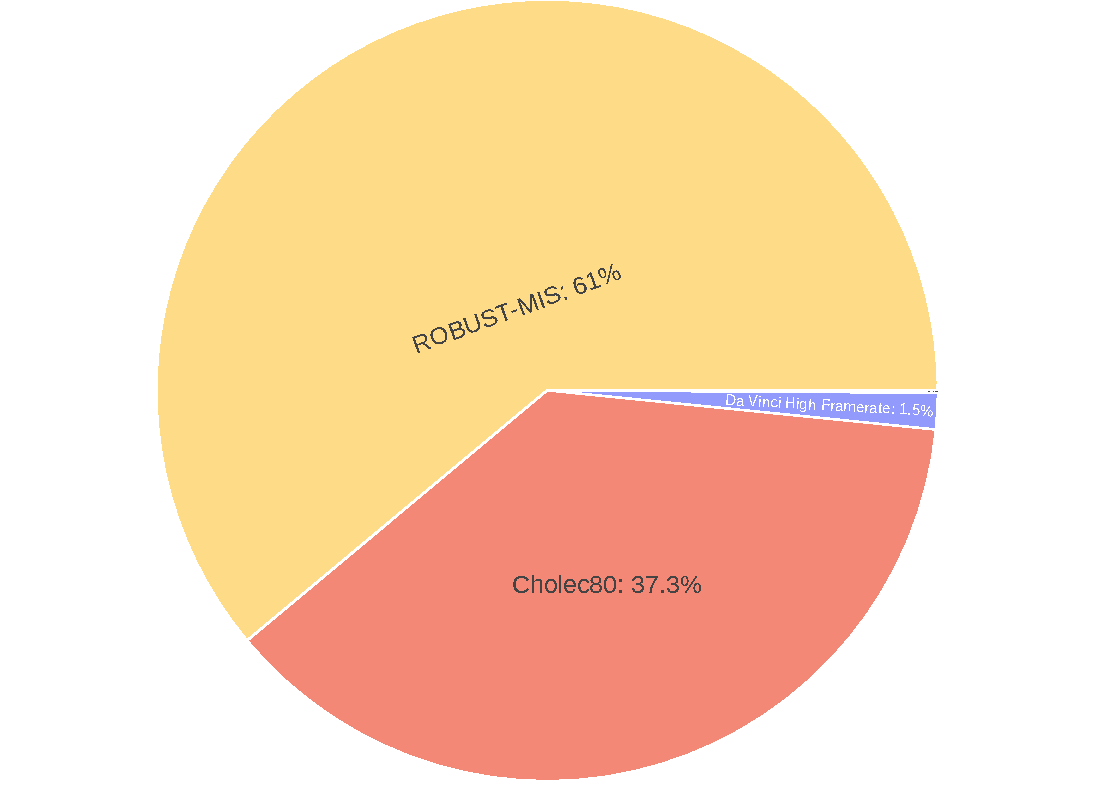
\includegraphics[width=1.\linewidth]{fig/fig_da_vinci_high_fps_laparoscopic.pdf}
% 		\caption{Laparoscopic datasets and a concatenation of the da Vinci\textsuperscript{\textregistered} high frame rate datasets. The ISAT dataset can barely be seen in this visualization. The Cholec80 dataset corresponds to about $51\,\text{h}$ of video.}
% 		\label{in:fig:da_vinci_laparoscopic}
% 	\end{subfigure}
% 	\caption{Dataset length visualizations for datasets listed in \tabref{in:tab:datasets}. Shown is the fraction of total number of images within a dataset.}
% 	\label{in:fig:datasets_sizes}
% \end{figure}

% $95\%$ of this data has no camera motion. We train all approaches from \secref{in:sec:implementation_homography_regression} on this data. We augment data with following probability
% \begin{itemize}
% 	\item Grayscale: $10\%$
% 	\item Horizontal flip: $50\%$
% 	\item Vertical flip: $50\%$
% 	\item Crop: $20\%$
% 	\item Brightness: $30\%$
% 	\item Gaussian blue: $10\%$
% 	\item Fog: $10\%$
% 	\item Contrast: $20\%$
% \end{itemize}
% Example augmentations are shown in \figref{in:fig:data_augmentation}. We train VGG-based networks and networks with a Resnet34~\cite{he2016deep} backbone. We use the Adam optimizer at a learning rate of $1\mathrm{e}{-4}$ and a momentum of $[0.9, 0.999]$. We set the batch size to $64$, the image crop shape to $480\times640$ and train for $20$ epochs on a train split with $80\%$ of the total data. The results are shown in \tabref{in:tab:train_results}. We excluded the results for the method from~\cite{zhang2019content}, as it converged to the trivial solution.
% \begin{table}[htb]
% 	\centering
% 	\caption{Test loss on high frame rate da Vinci\textsuperscript{\textregistered} dataset without camera motion.}
% 	\begin{tabular}{ccc}
% 		Architecture & Supervised & Mean Pairwise Distance / pixels\\
% 		\hline
% 		VGG~\cite{detone2016deep}         & yes & $4.547$ \\
% 		VGG~\cite{nguyen2018unsupervised} & no  & $5.875$ \\
% 		Resnet34                          & yes & $\mathbf{1.566}$ \\
% 		Resnet34                          & no  & $2.944$	
% 	\end{tabular}
% 	\label{in:tab:train_results}
% \end{table}
% The Resnet34-backboned network performs the best.
% \subsection{Homography Imitation Learning}
% \label{in:sec:homography_imitation_learning}
% To qualitatively assess the homography estimation capability of the Resnet34-backboned network, we perform inference on the unseen Cholec80 dataset. We do so as the Cholec80 dataset accounts for about $37\%$ of available laparoscopic data, see \figref{in:fig:da_vinci_laparoscopic}, and consists of continuous video, whereas the ROBUST-\gls{mis} dataset only comprises short video clips of length $10\,\text{s}$. We compare the deep method against a SIFT feature-based homography estimation method. Exemplary alpha blends are shown in \figref{in:fig:alpha_blend}. Example videos of the alignment with \href{https://drive.google.com/file/d/1SpUtSVgwo_PAwAjULF-Ky_5CxRuhMYlm/view?usp=sharing}{stride 1} and \href{https://drive.google.com/file/d/17fmhSsPq290PuLXmtO-aWwo3KN4QkZA8/view?usp=sharing}{stride 10} are also provided on Google Drive.

% \begin{figure}[htb]
% 	\centering
% 	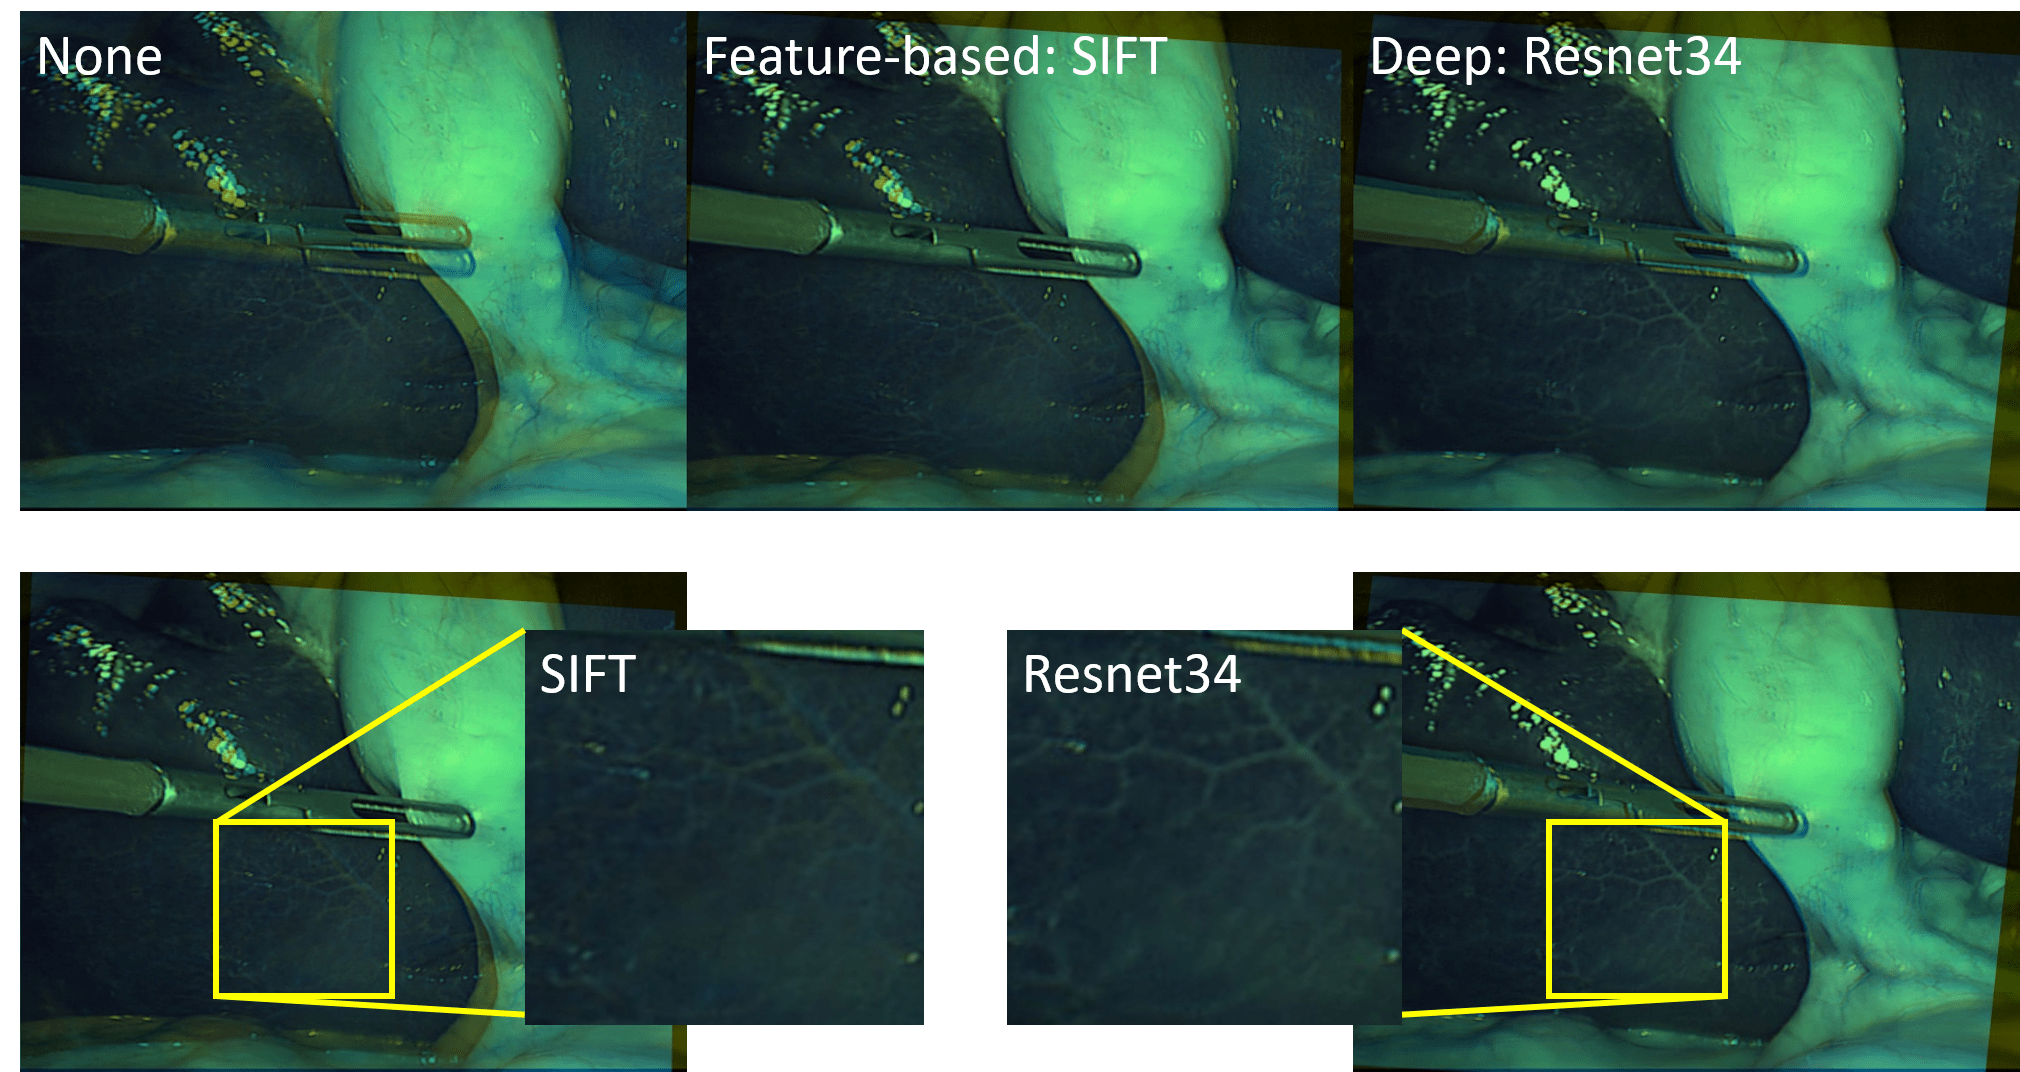
\includegraphics[width=.5\textwidth]{img/compresspng/blend_joint.png}
% 	\caption{Alpha blend of consecutive images from Cholec80 with stride $10$, corresponding to a $\Delta t$ of $0.4\,\text{s}$. Top row: The raw blend (none) shows severe camera and tool motion. The feature-based alignment breaks. The deep approach aligns both images well. Bottom row: The surgeon deforms the gallbladder while the camera is moving, the deep approach aligns the non-moving background well and ignores the deformation of the gallbladder, as can especially be seen in the zoom. Example videos of the alignment with \href{https://drive.google.com/file/d/1SpUtSVgwo_PAwAjULF-Ky_5CxRuhMYlm/view?usp=sharing}{stride 1} and \href{https://drive.google.com/file/d/17fmhSsPq290PuLXmtO-aWwo3KN4QkZA8/view?usp=sharing}{stride 10} are provided.}
% 	\label{in:fig:alpha_blend}
% \end{figure}

% Following the visual servo of \eqref{in:eq:twist}, we measure the severance of camera motion in a sequence of images by plotting the deviation of the estimated homography from the identity matrix against time, see \figref{in:fig:homography_annotation_moving_average}.

% \begin{figure}[htb]
% 	\centering
% 	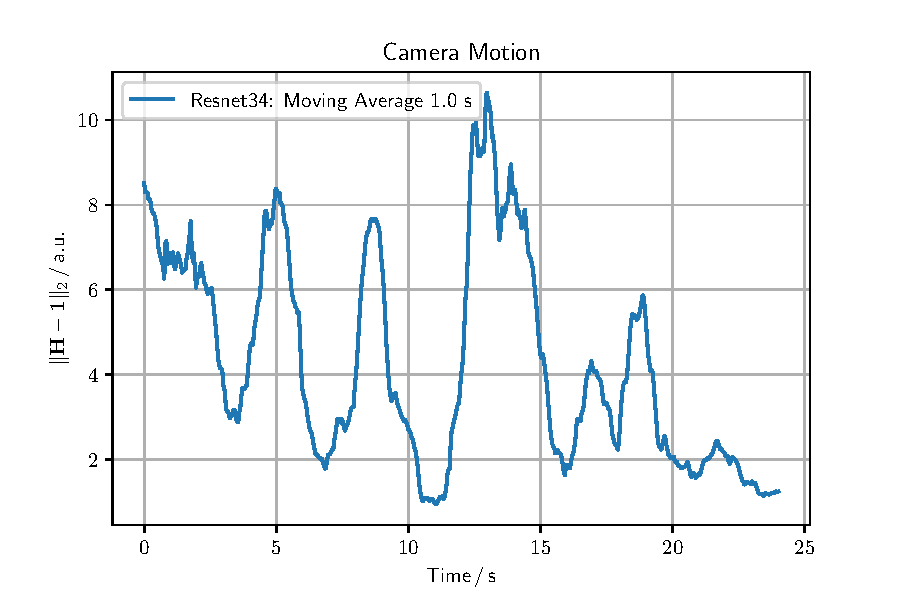
\includegraphics[width=.5\textwidth]{fig/homography_annotation_moving_average.pdf}
% 	\caption{Moving average of L2-norm of homography matrix identity deviation, similar to \eqref{in:eq:twist}. The homography was regressed in between consecutive images with stride 1 from Cholec80 using a Resnet34 backbone. The chosen metric reveals uncontinuous camera motion, as can be seen through alternating minima and maxima. This aligns well with the visual observation from video.}
% 	\label{in:fig:homography_annotation_moving_average}
% \end{figure}

% \section{OUTLOOK}
% \subsection{Conclusion}
% In this work, we are the first to combine a homography-based visual servo task with a remote center of motion objective as an enabler for deep-learning based control in robotic laparoscopic surgery. We implement said controller as a ROS package for use on any robot and demonstrate its effectiveness in \secref{in:sec:results_visual_servo}. We observe task convergence but also tip position divergence, see \figref{in:fig:visual_servo_measurements}. This is caused by the homography extraction from a distant calibration pattern, which is unresponsive to change in distance. We then generate a new dataset of da Vinci\textsuperscript{\textregistered} surgeries from which we isolate camera motion. We train multiple deep homography regression approaches and list results in \tabref{in:tab:train_results}. We find that, other than proposed in~\cite{detone2016deep}\cite{nguyen2018unsupervised}\cite{zhang2019content}, a Resnet34-backboned architecture performs the best. Based on this finding and on the dataset analysis in \figref{in:fig:da_vinci_laparoscopic}, we qualitatively evaluate the deep homography regression on the unseen dataset Cholec80 in \secref{in:sec:homography_imitation_learning}. We find central views within this data with a RANSAC method, see \figref{in:fig:ransac_circle}. We observe in \figref{in:fig:alpha_blend} that this method regresses camera motion well and isolates it from object motion. We also demonstrate the superiority over traditional SIFT feature-based homography estimation. Finally, we show in \figref{in:fig:homography_annotation_moving_average} that the homography regression can be used to reveal uncontinuous camera motion in video data, which aligns well with visual observation.
% \subsection{Shortcomings and Future Work}
% Although we demonstrate future potential for the presented approach, there are still shortcomings that are yet to be addressed. The results for the visual servo were taken from simulation, the toy calibration pattern homography extraction does not yet run on the real setup. The toy homography extraction also showed diverging properties for the tip of the laparoscope in simulation, which will be addressed by replacing the type homography extraction in the future. We further note that many of the homography regression results are not yet backed by quantitative measures. This will be accounted for by creating a human-labelled ground truth data subset. To now achieve an autonomous robotic endoscope, we will extend the work starting from \figref{in:fig:homography_annotation_moving_average}, where the potential of a next best view planning was revealed from the data at hand. We will further implement a force control on the real robot for feedback to extend the pipeline into an active learning approach.
